% !TeX spellcheck = pl_PL
%%%%%%%%%%%%%%%%%%%%%%%%%%%%%%%%%%%%%%%%%%%
%                                        %
% Szablon pracy dyplomowej inzynierskiej %
% zgodny  z aktualnymi  przepisami  SZJK %
%                                        %
%%%%%%%%%%%%%%%%%%%%%%%%%%%%%%%%%%%%%%%%%%
%                                        %
%  (c) Krzysztof Simiński, 2018-2023     %
%                                        %
%%%%%%%%%%%%%%%%%%%%%%%%%%%%%%%%%%%%%%%%%%
%                                        %
% Najnowsza wersja szablonów jest        %
% podstępna pod adresem                  %
% github.com/ksiminski/polsl-aei-theses  %
%                                        %
%%%%%%%%%%%%%%%%%%%%%%%%%%%%%%%%%%%%%%%%%%
%
%
% Projekt LaTeXowy zapewnia odpowiednie formatowanie pracy,
% zgodnie z wymaganiami Systemu zapewniania jakości kształcenia.
% Proszę nie zmieniać ustawień formatowania (np. fontu,
% marginesów, wytłuszczeń, kursywy itd. ).
%
% Projekt można kompilować na kilka sposobów.
%
% 1. kompilacja pdfLaTeX
%
% pdflatex main
% bibtex   main
% pdflatex main
% pdflatex main
%
%
% 2. kompilacja XeLaTeX
%
% Kompilatacja przy użyciu XeLaTeXa różni się tym, że na stronie
% tytułowej używany jest font Calibri. Wymaga to jego uprzedniego
% zainstalowania.
%
% xelatex main
% bibtex  main
% xelatex main
% xelatex main
%
%
%%%%%%%%%%%%%%%%%%%%%%%%%%%%%%%%%%%%%%%%%%%%%%%%%%%%%
% W przypadku pytań, uwag, proszę pisać na adres:   %
%      krzysztof.siminski(małpa)polsl.pl            %
%%%%%%%%%%%%%%%%%%%%%%%%%%%%%%%%%%%%%%%%%%%%%%%%%%%%%
%
% Chcemy ulepszać szablony LaTeXowe prac dyplomowych.
% Wypełniając ankietę spod poniższego adresu pomogą
% Państwo nam to zrobić. Ankieta jest całkowicie
% anonimowa. Dziękujemy!


% https://docs.google.com/forms/d/e/1FAIpQLScyllVxNKzKFHfILDfdbwC-jvT8YL0RSTFs-s27UGw9CKn-fQ/viewform?usp=sf_link
%
%%%%%%%%%%%%%%%%%%%%%%%%%%%%%%%%%%%%%%%%%%%%%%%%%%%%%%%%%%%%%%%%%%%%%%%%%

%%%%%%%%%%%%%%%%%%%%%%%%%%%%%%%%%%%%%%%%%%%%%%%
%                                             %
% PERSONALIZACJA PRACY – DANE PRACY           %
%                                             %
%%%%%%%%%%%%%%%%%%%%%%%%%%%%%%%%%%%%%%%%%%%%%%%

% Proszę wpisać swoje dane w poniższych definicjach.

% TODO
% dane autora
\newcommand{\FirstNameAuthor}{Imię}
\newcommand{\SurnameAuthor}{Nazwisko}
\newcommand{\IdAuthor}{$\langle$wpisać właściwy$\rangle$}   % numer albumu  (bez $\langle$ i $\rangle$)

% drugi autor:
%\newcommand{\FirstNameCoauthor}{Imię}   % Jeżeli jest drugi autor, to tutaj należy podać imię.
%\newcommand{\SurnameCoauthor}{Nazwisko} % Jeżeli jest drugi autor, to tutaj należy podać nazwisko.
%\newcommand{\IdCoauthor}{$\langle$wpisać właściwy$\rangle$}  % numer albumu drugiego autora (bez $\langle$ i $\rangle$)
% Gdy nie ma drugiego autora, należy zostawić poniższe definicje puste, jak poniżej. Gdy jest drugi autor, należy zakomentować te linie.
\newcommand{\FirstNameCoauthor}{} % Jeżeli praca ma tylko jednego autora, to dane drugiego autora zostają puste.
\newcommand{\SurnameCoauthor}{}   % Jeżeli praca ma tylko jednego autora, to dane drugiego autora zostają puste.
\newcommand{\IdCoauthor}{}  % Jeżeli praca ma tylko jednego autora, to dane drugiego autora zostają puste.
%%%%%%%%%%

\newcommand{\Supervisor}{$\langle$tytuł lub stopień naukowy oraz imię i nazwisko$\rangle$}     % dane promotora (bez $\langle$ i $\rangle$)
\newcommand{\Title}{Postcardia - Aplikacja społecznościowa do kolekcjonowania i wysyłania pocztówek}           % tytuł pracy po polsku
\newcommand{\TitleAlt}{Postcardia - Community application for collecting and sending postcards}                     % thesis title in English
\newcommand{\Program}{$\langle$wpisać właściwy$\rangle$}            % kierunek studiów  (bez $\langle$ i $\rangle$)
\newcommand{\Specialisation}{$\langle$wpisać właściwą$\rangle$}     % specjalność  (bez $\langle$ i $\rangle$)
\newcommand{\Departament}{$\langle$wpisać właściwą$\rangle$}        % katedra promotora  (bez $\langle$ i $\rangle$)

% Jeżeli został wyznaczony promotor pomocniczy lub opiekun, proszę go/ją wpisać ...
\newcommand{\Consultant}{$\langle$stopień naukowy imię i nazwisko$\rangle$} % dane promotora pomocniczego, opiekuna (bez $\langle$ i $\rangle$)
% ... w przeciwnym razie proszę zostawić puste miejsce jak poniżej:
%\newcommand{\Consultant}{} % brak promotowa pomocniczego / opiekuna

% koniec fragmentu do modyfikacji
%%%%%%%%%%%%%%%%%%%%%%%%%%%%%%%%%%%%%%%%%%


%%%%%%%%%%%%%%%%%%%%%%%%%%%%%%%%%%%%%%%%%%%%%%%
%                                             %
% KONIEC PERSONALIZACJI PRACY                 %
%                                             %
%%%%%%%%%%%%%%%%%%%%%%%%%%%%%%%%%%%%%%%%%%%%%%%

%%%%%%%%%%%%%%%%%%%%%%%%%%%%%%%%%%%%%%%%


%%%%%%%%%%%%%%%%%%%%%%%%%%%%%%%%%%%%%%%%%%%%%%%
%                                             %
% PROSZĘ NIE MODYFIKOWAĆ PONIŻSZYCH USTAWIEŃ! %
%                                             %
%%%%%%%%%%%%%%%%%%%%%%%%%%%%%%%%%%%%%%%%%%%%%%%



\documentclass[a4paper,twoside,12pt]{book}
\usepackage[utf8]{inputenc}                                      
\usepackage[T1]{fontenc}  
\usepackage{amsmath,amsfonts,amssymb,amsthm}
\usepackage[british,polish]{babel} 
\usepackage{indentfirst}
\usepackage{xurl}
\usepackage{xstring}
\usepackage{ifthen}
\usepackage{float}



\usepackage{ifxetex}

\ifxetex
	\usepackage{fontspec}
	\defaultfontfeatures{Mapping=tex—text} % to support TeX conventions like ``——-''
	\usepackage{xunicode} % Unicode support for LaTeX character names (accents, European chars, etc)
	\usepackage{xltxtra} % Extra customizations for XeLaTeX
\else
	\usepackage{lmodern}
\fi



\usepackage[margin=2.5cm]{geometry}
\usepackage{graphicx} 
\usepackage{hyperref}
\usepackage{booktabs}
\usepackage{tikz}
\usepackage{pgfplots}
\usepackage{mathtools}
\usepackage{geometry}
\usepackage{subcaption}   % subfigures
\usepackage[page]{appendix} % toc,
\renewcommand{\appendixtocname}{Dodatki}
\renewcommand{\appendixpagename}{Dodatki}
\renewcommand{\appendixname}{Dodatek}

\usepackage{csquotes}
\usepackage[natbib=true,backend=bibtex,maxbibnames=99]{biblatex}  % kompilacja bibliografii BibTeXem
%\usepackage[natbib=true,backend=biber,maxbibnames=99]{biblatex}  % kompilacja bibliografii Biberem
\bibliography{biblio}

\usepackage{ifmtarg}   % empty commands  

\usepackage{setspace}
\onehalfspacing


\frenchspacing



%%%% TODO LIST GENERATOR %%%%%%%%%

\usepackage{color}
\definecolor{brickred}      {cmyk}{0   , 0.89, 0.94, 0.28}

\makeatletter \newcommand \kslistofremarks{\section*{Uwagi} \@starttoc{rks}}
  \newcommand\l@uwagas[2]
    {\par\noindent \textbf{#2:} %\parbox{10cm}
{#1}\par} \makeatother


\newcommand{\ksremark}[1]{%
{%\marginpar{\textdbend}
{\color{brickred}{[#1]}}}%
\addcontentsline{rks}{uwagas}{\protect{#1}}%
}

\newcommand{\comma}{\ksremark{przecinek}}
\newcommand{\nocomma}{\ksremark{bez przecinka}}
\newcommand{\styl}{\ksremark{styl}}
\newcommand{\ortografia}{\ksremark{ortografia}}
\newcommand{\fleksja}{\ksremark{fleksja}}
\newcommand{\pauza}{\ksremark{pauza `--', nie dywiz `-'}}
\newcommand{\kolokwializm}{\ksremark{kolokwializm}}
\newcommand{\cudzyslowy}{\ksremark{,,polskie cudzysłowy''}}

%%%%%%%%%%%%%% END OF TODO LIST GENERATOR %%%%%%%%%%%

\newcommand{\printCoauthor}{%		
    \StrLen{\FirstNameCoauthor}[\FNCoALen]
    \ifthenelse{\FNCoALen > 0}%
    {%
		{\large\bfseries\Coauthor\par}
	
		{\normalsize\bfseries \LeftId: \IdCoauthor\par}
    }%
    {}
} 

%%%%%%%%%%%%%%%%%%%%%
\newcommand{\autor}{%		
    \StrLen{\FirstNameCoauthor}[\FNCoALenXX]
    \ifthenelse{\FNCoALenXX > 0}%
    {\FirstNameAuthor\ \SurnameAuthor, \FirstNameCoauthor\ \SurnameCoauthor}%
	{\FirstNameAuthor\ \SurnameAuthor}%
}
%%%%%%%%%%%%%%%%%%%%%

\StrLen{\FirstNameCoauthor}[\FNCoALen]
\ifthenelse{\FNCoALen > 0}%
{%
\author{\FirstNameAuthor\ \SurnameAuthor, \FirstNameCoauthor\ \SurnameCoauthor}
}%
{%
\author{\FirstNameAuthor\ \SurnameAuthor}
}%

%%%%%%%%%%%% ZYWA PAGINA %%%%%%%%%%%%%%%
% brak kapitalizacji zywej paginy
\usepackage{fancyhdr}
\pagestyle{fancy}
\fancyhf{}
\fancyhead[LO]{\nouppercase{\it\rightmark}}
\fancyhead[RE]{\nouppercase{\it\leftmark}}
\fancyhead[LE,RO]{\it\thepage}


\fancypagestyle{tylkoNumeryStron}{%
   \fancyhf{} 
   \fancyhead[LE,RO]{\it\thepage}
}

\fancypagestyle{bezNumeracji}{%
   \fancyhf{} 
   \fancyhead[LE,RO]{}
}


\fancypagestyle{NumeryStronNazwyRozdzialow}{%
   \fancyhf{} 
   \fancyhead[LE]{\nouppercase{\autor}}
   \fancyhead[RO]{\nouppercase{\leftmark}} 
   \fancyfoot[CE, CO]{\thepage}
}


%%%%%%%%%%%%% OBCE WTRETY  
\newcommand{\obcy}[1]{\emph{#1}}
\newcommand{\english}[1]{{\selectlanguage{british}\obcy{#1}}}
%%%%%%%%%%%%%%%%%%%%%%%%%%%%%

% polskie oznaczenia funkcji matematycznych
\renewcommand{\tan}{\operatorname {tg}}
\renewcommand{\log}{\operatorname {lg}}

% jeszcze jakies drobiazgi

\newcounter{stronyPozaNumeracja}

%%%%%%%%%%%%%%%%%%%%%%%%%%% 
\newcommand{\printOpiekun}[1]{%		

    \StrLen{\Consultant}[\mystringlen]
    \ifthenelse{\mystringlen > 0}%
    {%
       {\large{\bfseries OPIEKUN, PROMOTOR POMOCNICZY}\par}
       
       {\large{\bfseries \Consultant}\par}
    }%
    {}
} 
%
%%%%%%%%%%%%%%%%%%%%%%%%%%%%%%%%%%%%%%%%%%%%%%
 
% Proszę nie modyfikować poniższych definicji!
\newcommand{\Author}{\FirstNameAuthor\ \MakeUppercase{\SurnameAuthor}} 
\newcommand{\Coauthor}{\FirstNameCoauthor\ \MakeUppercase{\SurnameCoauthor}}
\newcommand{\Type}{PROJEKT INŻYNIERSKI}
\newcommand{\Faculty}{Wydział Matematyki Stosowanej} 
\newcommand{\Polsl}{Politechnika Śląska}
\newcommand{\Logo}{politechnika_sl_logo_bw_pion_pl.pdf}
\newcommand{\LeftId}{Nr albumu}
\newcommand{\LeftProgram}{Kierunek}
\newcommand{\LeftSpecialisation}{Specjalność}
\newcommand{\LeftSUPERVISOR}{PROWADZĄCY PRACĘ}
\newcommand{\LeftDEPARTMENT}{KATEDRA}
%%%%%%%%%%%%%%%%%%%%%%%%%%%%%%%%%%%%%%%%%%%%%%

%%%%%%%%%%%%%%%%%%%%%%%%%%%%%%%%%%%%%%%%%%%%%%%
%                                             %
% KONIEC USTAWIEŃ                             %
%                                             %
%%%%%%%%%%%%%%%%%%%%%%%%%%%%%%%%%%%%%%%%%%%%%%%




%%%%%%%%%%%%%%%%%%%%%%%%%%%%%%%%%%%%%%%%%%%%%%%
%                                             %
% MOJE PAKIETY, USTAWIENIA ITD                %
%                                             %
%%%%%%%%%%%%%%%%%%%%%%%%%%%%%%%%%%%%%%%%%%%%%%%

% Tutaj proszę umieszczać swoje pakiety, makra, ustawienia itd.


 
%%%%%%%%%%%%%%%%%%%%%%%%%%%%%%%%%%%%%%%%%%%%%%%%%%%%%%%%%%%%%%%%%%%%%
% listingi i fragmentu kodu źródłowego 
% pakiet: listings lub minted
% % % % % % % % % % % % % % % % % % % % % % % % % % % % % % % % % % % 

% biblioteka listings
%stare
% \usepackage{listings}
% \lstset{%
% morekeywords={string,exception,std,vector},% słowa kluczowe rozpoznawane przez pakiet listings
% language=C++,% C, Matlab, Python, SQL, TeX, XML, bash, ... – vide https://www.ctan.org/pkg/listings
% commentstyle=\textit,%
% identifierstyle=\textsf,%
% keywordstyle=\sffamily\bfseries, %\texttt, %
% %captionpos=b,%
% tabsize=3,%
% frame=lines,%
% numbers=left,%
% numberstyle=\tiny,%
% numbersep=5pt,%
% breaklines=true,%
% escapeinside={@*}{*@},%
% }

% biblioteka listings - NOWE
\usepackage{listings}
\usepackage{xcolor}

\definecolor{codegreen}{rgb}{0,0.6,0}
\definecolor{codegray}{rgb}{0.5,0.5,0.5}
\definecolor{codepurple}{rgb}{0.58,0,0.82}
\definecolor{backcolour}{rgb}{0.95,0.95,0.92}
\definecolor{codeorange}{rgb}{1,0.647,0}
\definecolor{codeblue}{rgb}{0,0,1}

\lstset{%
    morekeywords={string,exception,std,vector},% słowa kluczowe rozpoznawane przez pakiet listings
    language=C++,% C, Matlab, Python, SQL, TeX, XML, bash, ... – vide https://www.ctan.org/pkg/listings
    commentstyle=\textit{\color{codegreen}},%
    identifierstyle=\textsf{\color{codegray}},%
    keywordstyle=[1]\sffamily\bfseries\color{codepurple},%
    keywordstyle=[2]\sffamily\bfseries\color{codeorange},%
    keywordstyle=[3]\sffamily\bfseries\color{codeblue},%
    backgroundcolor=\color{backcolour},
    %captionpos=b,%
    tabsize=3,%
    frame=lines,%
    numbers=left,%
    numberstyle=\tiny\color{codegray},%
    numbersep=5pt,%
    breaklines=true,%
    escapeinside={@*}{*@},%
}

% % % % % % % % % % % % % % % % % % % % % % % % % % % % % % % % % % % 
% pakiet minted
%\usepackage{minted}

% pakiet wymaga specjalnego kompilowania:
% pdflatex -shell-escape main.tex
% xelatex  -shell-escape main.tex

%\usepackage[chapter]{minted} % [section]
%%\usemintedstyle{bw}   % czarno-białe kody 
%
%\setminted % https://ctan.org/pkg/minted
%{
%%fontsize=\normalsize,%\footnotesize,
%%captionpos=b,%
%tabsize=3,%
%frame=lines,%
%framesep=2mm,
%numbers=left,%
%numbersep=5pt,%
%breaklines=true,%
%escapeinside=@@,%
%}

%%%%%%%%%%%%%%%%%%%%%%%%%%%%%%%%%%%%%%%%%%%%%%%%%%%%%%%%%%%%%%%%%%%%%



%%%%%%%%%%%%%%%%%%%%%%%%%%%%%%%%%%%%%%%%%%%%%%%
%                                             %
% KONIEC MOICH USTAWIEŃ                       %
%                                             %
%%%%%%%%%%%%%%%%%%%%%%%%%%%%%%%%%%%%%%%%%%%%%%%



%%%%%%%%%%%%%%%%%%%%%%%%%%%%%%%%%%%%%%%%


\begin{document}
%\kslistofremarks

\frontmatter

%%%%%%%%%%%%%%%%%%%%%%%%%%%%%%%%%%%%%%%%%%%%%%%
%                                             %
% PROSZĘ NIE MODYFIKOWAĆ STRONY TYTUŁOWEJ!    %
%                                             %
%%%%%%%%%%%%%%%%%%%%%%%%%%%%%%%%%%%%%%%%%%%%%%%


%%%%%%%%%%%%%%%%%%  STRONA TYTUŁOWA %%%%%%%%%%%%%%%%%%%
\pagestyle{empty}
{
	\newgeometry{top=1.5cm,%
	             bottom=2.5cm,%
	             left=3cm,
	             right=2.5cm}
 
	\ifxetex 
	  \begingroup
	  \setsansfont{Calibri}
	   
	\fi 
	 \sffamily
	\begin{center}
	\includegraphics[width=50mm]{\Logo}
	 
	
	{\Large\bfseries\Type\par}
	
	\vfill  \vfill  
			 
	{\large\Title\par}
	
	\vfill  
		
	{\large\bfseries\Author\par}
	
	{\normalsize\bfseries \LeftId: \IdAuthor}

	\printCoauthor
	
	\vfill  		
 
	{\large{\bfseries \LeftProgram:} \Program\par} 
	
	{\large{\bfseries \LeftSpecialisation:} \Specialisation\par} 
	 		
	\vfill  \vfill 	\vfill 	\vfill 	\vfill 	\vfill 	\vfill  
	 
	{\large{\bfseries \LeftSUPERVISOR}\par}
	
	{\large{\bfseries \Supervisor}\par}
				
	{\large{\bfseries \LeftDEPARTMENT\ \Departament} \par}
		
	{\large{\bfseries \Faculty}\par}
		
	\vfill  \vfill  

    	
    \printOpiekun{\Consultant}
    
	\vfill  \vfill  
		
    {\large\bfseries  Gliwice \the\year}

   \end{center}	
       \ifxetex 
       	  \endgroup
       \fi
	\restoregeometry
}
  
%%%%%%%%%%%%%%%%%%%%%%%%%%%%%%%%%%%%%%%%%%%%%%%
%                                             %
% KONIEC STRONY TYTUŁOWEJ                     %
%                                             %
%%%%%%%%%%%%%%%%%%%%%%%%%%%%%%%%%%%%%%%%%%%%%%%  


\cleardoublepage

\rmfamily\normalfont
\pagestyle{empty}


%%% No to zaczynamy pisać pracę :-) %%%%

% TODO
\subsubsection*{Tytuł pracy} 
\Title

\subsubsection*{Streszczenie}  
Praca prezentuje rezultaty oraz proces tworzenia aplikacji społecznościowej której głównym celem jest kolekcjonowanie oraz wysyłanie pocztówek z odwiedzonych miejsc. Głównym trzonem aplikacji jest jej część mobilna oparta na platformie Flutter, której działanie wspierane jest poprzez dedykowaną aplikację serwerową wykorzystującą technologię .NET. Dodatkowo aplikacja zawiera także oddzielną część webową wykorzystującą technologię React, część ta korzysta z tej samej aplikacji serwerowej co aplikacja mobilna.

\subsubsection*{Słowa kluczowe} 
Flutter, .NET, React, CRUD, Pocztówki, Aplikacja społecznościowa, Zwiedzanie

\subsubsection*{Thesis title} 
\begin{otherlanguage}{british}
\TitleAlt
\end{otherlanguage}

\subsubsection*{Abstract} 
\begin{otherlanguage}{british}
The thesis presents the results and the process of creating a social application whose main purpose is to collect and send postcards from visited places. The core of the application is its mobile component built on the Flutter platform, supported by a dedicated server application utilizing .NET technology. Additionally, the application includes a separate web component using React technology, and this web part utilizes the same server application as the mobile application.
\end{otherlanguage}
\subsubsection*{Key words}  
\begin{otherlanguage}{british}
Flutter, .NET, React, CRUD, Postcards, Community app, Touring
\end{otherlanguage}




%%%%%%%%%%%%%%%%%% SPIS TRESCI %%%%%%%%%%%%%%%%%%%%%%
% Add \thispagestyle{empty} to the toc file (main.toc), because \pagestyle{empty} doesn't work if the TOC has multiple pages
\addtocontents{toc}{\protect\thispagestyle{empty}}
\tableofcontents

%%%%%%%%%%%%%%%%%%%%%%%%%%%%%%%%%%%%%%%%%%%%%%%%%%%%%
\setcounter{stronyPozaNumeracja}{\value{page}}
\mainmatter
\pagestyle{empty}

\cleardoublepage

\pagestyle{NumeryStronNazwyRozdzialow}

%%%%%%%%%%%%%% wlasciwa tresc pracy %%%%%%%%%%%%%%%%%

% TODO
\chapter{Wstęp}
\label{ch:wstep}

\section{Wprowadzenie}
% Aplikacje społecznościowe w dzisiejszym świecie są dla czymś powszechnym. Większość z nich sprowadza się do wysyłania zdjęć oraz wymieniania wiadomości. Przed erą smartfonów takie informacje były bardziej spersonalizowane, ponieważ służyły do tego listy na których pisaliśmy co robimy, oraz pocztówki dzięki którym mogliśmy pokazać gdzie jesteśmy. Właśnie to drugie zainspirowało nas do połączenia starego z nowym - pocztówek z aplikacją społecznościową. Chcemy, aby odwiedzanie różnych miejsc, czy to lokalnie, blisko, czy tych na drugim końcu świata, łączyło się z czymś kiedyś powszechnym czyli wysyłaniem pocztówek. Wszak cieszymy się bardziej z pocztówki wysłanej przez rodzinę lub przyjaciela niż ze zdjęcia na Facebooku. 

Aplikacje społecznościowe w dzisiejszym świecie są dla czymś powszechnym. Większość z nich sprowadza się do wysyłania zdjęć oraz wymieniania wiadomości.  Przed erą smartfonów takie informacje były bardziej spersonalizowane, ponieważ służyły do tego listy na których pisaliśmy co robimy, oraz pocztówki dzięki którym mogliśmy pokazać gdzie jesteśmy. Właśnie to drugie zainspirowało nas do połączenia starego z nowym - pocztówek z aplikacją społecznościową.

Chcemy, aby podróżowanie i odwiedzanie różnych miejsc, zarówno lokalnych, blisko, jak i tych na drugim końcu świata, było związane z czymś kiedyś powszechnym - wysyłaniem pocztówek. Wszyscy z pewnością cieszymy się bardziej z pocztówki wysłanej przez kogoś nam bliskiego niż ze zwykłego zdjęcia na znanym portalu społecznościowym. W związku z tym nasza aplikacja umożliwia użytkownikom odbieranie wirtualnych pocztówek podczas odwiedzania ciekawych miejsc. Później te elektroniczne pocztówki można przesłać innym osobom jako miłe wiadomości lub po prostu w celach kolekcjonerskich.

Ze względu na ograniczoną ilość osób, którym możemy przekazać wirtualne pocztówki, każda z nich staje się wyjątkowa i posiada większą wartość dla odbiorcy niż wcześniej wspomniane zdjęcie na tablicy popularnego portalu społecznościowego. Nasza aplikacja stanowi również doskonały sposób na poszerzenie kolekcji miejsc, które użytkownik odwiedził.

\newpage

\section{Cel pracy}
Celem naszej pracy jest stworzenie wyjątkowej w pełni działającej aplikacji mobilnej umożliwiającej na zawiązywanie znajomości, wymianę oraz kolekcjonowanie pocztówek z odwiedzonych miejsc. Dodatkowo celem jest stworzenie aplikacji webowej umożliwiającą wykonanie większości czynności z~aplikacji mobilnej, jak i również backendu działającego na obu platformach odpowiedzialnego za część serwerową. Aplikacja mobilna oraz webowa powinna być intuicyjna i łatwa w obsłudze, oraz zachęcać użytkowników do aktywnego wypoczynku (zwiedzania) oraz rozwijania się w aspekcie społecznym poprzez wysyłanie oraz odbieranie wyjątkowych pocztówek z różnych ciekawych miejsc w okolicy jak i na całym świecie.

\section{Zakres pracy}
Zakres pracy obejmował zaprojektowanie intuicyjnej i wyjątkowej aplikacji składającej się z trzech głównych modułów oraz jej kompleksową implementację.
\\
Poszczególne moduły:
\begin{itemize}
    \item Aplikacji mobilnej stworzonej w technologi Flutter.
    \item Aplikacji serwerowej stworzonej w technologi .Net.
    \item Aplikacji webowej stworzonej w technologi React.
\end{itemize}

Przed przejściem do fazy implementacji w każdym module najpierw przeprowadzono fazę projektowania, mającą na celu ocenę sensowności oraz zdefiniowanie kluczowych aspektów modułu. 

Zakres pracy przewidywał także przeprowadzenie odpowiednich testów jak i analizę jakości utworzonego projektu oraz stworzenie szczegółowej dokumentacji technicznej opisującej działanie, architekturę i wykorzystane technologie.

\newpage

\section{Zwięzła charakterystyka rozdziałów}
\begin{itemize}
    \item \textbf{Rozdział 1:} Wstęp -- Zaprezentowanie ogólnego kontekstu oraz celów pracy
    \item \textbf{Rozdział 2:} Analiza tematu -- W tym rozdziale przedstawiony zostanie problem, poszczególne podobne aplikacje oraz rozwiązania z rzeczywistości, nakreślenie przykładowego profilu konsumenta aplikacji oraz przedstawienie wyróżniających nasz projekt rozwiązań
    \item \textbf{Rozdział 3:} Wymagania -- Przedstawienie wymagań funkcjonalnych jak i niefunkcjonalnych
    \item \textbf{Rozdział 4:} Metodyka pracy nad projektowaniem i implementacją -- opis wykorzystanej metodyki podczas fazy projektowania jak i implementacji, użyte narzędzia, pomysły, workflow w projekcie
    \item \textbf{Rozdział 5:} Aplikacja mobilna -- Szeroki opis dotyczący aplikacji mobilnej, wykorzystanych bibliotek, zastosowanej architektury jak i instrukcja obsługi
    \item \textbf{Rozdział 6:} Aplikacja serwerowa -- Szeroki opis dotyczący aplikacji serwerowej, wykorzystanych technilogii oraz platform, zastosowanej architektury  oraz struktury, wykorzystane modele, szczegóły dotyczące specyfikacji oraz funkcjonalności. Przeprowadzone testy automatyczne oraz manualne
    \item \textbf{Rozdział 7:} Aplikacja webowa -- TODO
    \item \textbf{Rozdział 8:} Podsumowanie i wnioski -- Przedstawienie potencjalnego sposobu na dalszy rozwój aplikacji, omówienie napotkanych problemów i trudności podczas tworzenia jak i projektowania aplikacji, wyciągnięcie wniosków w świetle postawionych wcześniej celów i wymagań
\end{itemize}

\newpage

\section{Autorzy}
Aplikacja była tworzona przez czteroosobowy zespół w którego skład wchodzili: 
\begin{itemize}
    \item Patryk Sroczyński
    \item Arkadiusz Stencel
    \item Dawid Strzyż
    \item Mariusz Wróbel
\end{itemize}

Początkowo najwięcej zasobów ludzkich zostało przeznaczonych na stworzenie aplikacji mobilnej, która docelowo miała być głównym produktem projektu. Ze względu na sprawny przebieg prac w części mobilnej oraz serwerowej, część osób została oddelegowana do pomocy z aplikacją webową. Szczegóły przedstawia poniższa tabela:
\begin{table}[ht]
\centering
\begin{tabular}{|c|c|c|c|}
\hline
\textbf{Osoba} & \textbf{Część mobilna} & \textbf{Część webowa} & \textbf{Część serwerowa} \\ \hline
\textbf{Patryk Sroczyński}    &               & Pomoc            & Głównie      \\ \hline
\textbf{Arkadiusz Stencel}    & Głównie       &                  &              \\ \hline
\textbf{Dawid Strzyż}         &               & Głównie          &              \\ \hline
\textbf{Mariusz Wróbel}       & Głównie       & Pomoc            &              \\ \hline
\end{tabular}
\caption{Autorstwo poszczególnych elementów pracy.}
\end{table}


% TODO
\chapter{Analiza tematu}

\section{Sformułowanie problemu}
Wraz z rozwojem technologicznym media społecznościowe odgrywają coraz to większą rolę w naszym społeczeństwie a dawne tradycje zaczynają tracić na wartości. Media społecznościowe w większości wypadków nie propagują zdrowego trybu życia a jedynie ciągłe siedzenie w miejscu i przewijanie kolejnych treści. Dlatego zadaliśmy sobie pytanie czy można stworzyć aplikację łączącą tradycyjne zwyczaje z nowoczesnym podejściem która jednocześnie pozwala na bardziej aktywne spędzanie czasu.

\begin{figure}[H]
    \centering
    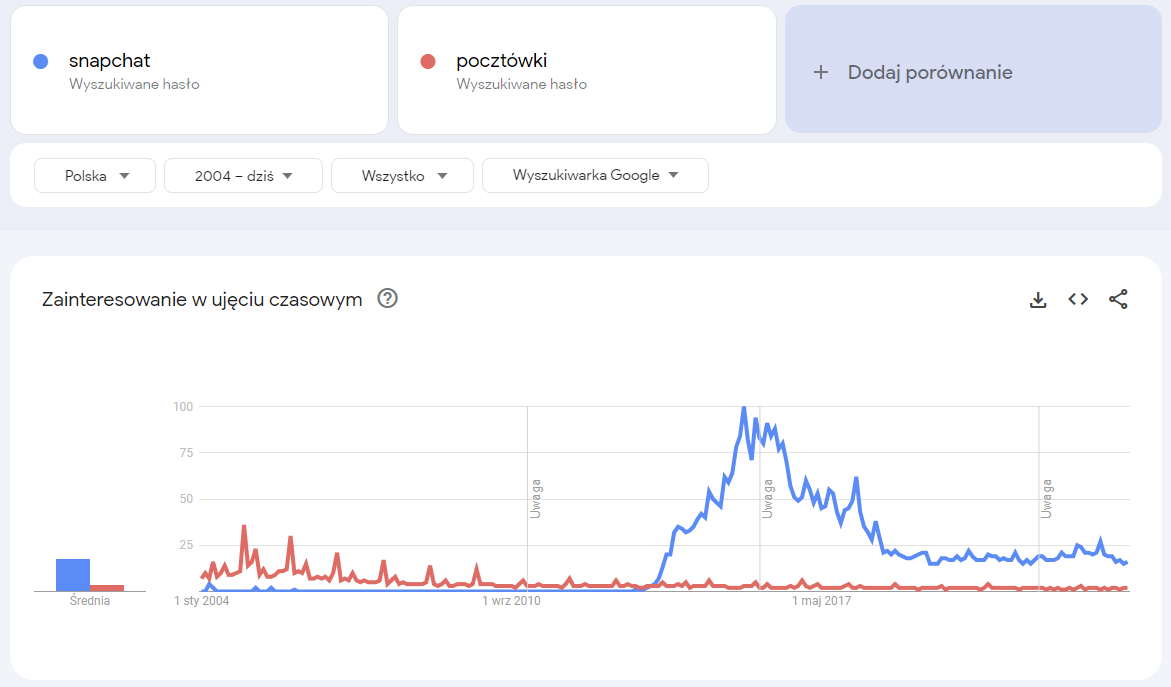
\includegraphics[width=1\textwidth]{porownanie.png}
    \caption{Zestawienie zainteresowania pomiędzy słowem kluczowym Snapchat a pocztówki na przestrzeni lat - źródło Google trends}
\end{figure}

\newpage
\section{Przegląd podobnych aplikacji oraz rozwiązań}
\subsection{Snapchat}
Snapchat to aplikacja społecznościowa dzięki której użytkownicy mogą wysyłać zdjęcia lub filmy konkretnym osobom lub całym grupom, aplikacja pozwala także na dodawanie specjalnych filtrów (na przykład dodanie naklejki z lokalizacji w której zdjęcie zostało stworzone) lub tekstu do przesyłanych treści, elementem specyficznym dla tej aplikacji jest to że odtworzenie czyjejś wiadomości powoduje jej zniknięcie po określonym czasie.
Snapchat swój rekord popularności zarejestrował w latach 2015-2016, lecz mimo to do dzisiaj aplikacja cieszy się wielką popularnością szczególnie wśród młodych ludzi.
\begin{figure}[H]
    \centering
    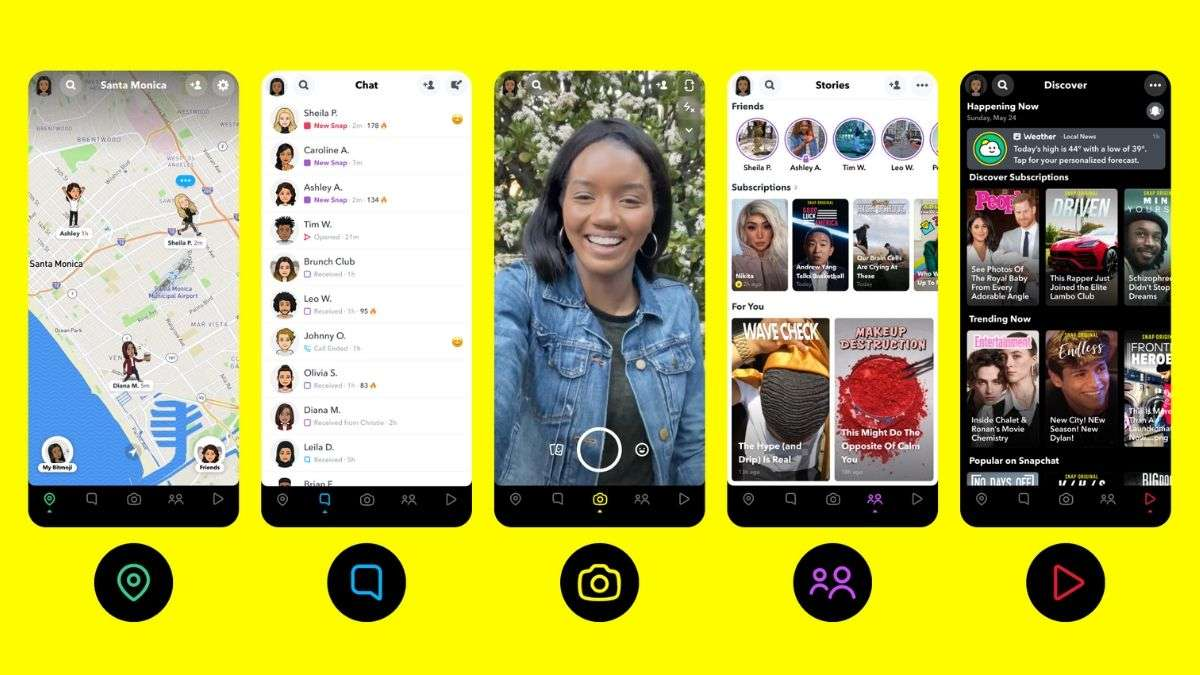
\includegraphics[width=1\textwidth]{apki_ss/snapchat.jpg}
    \caption{Snapchat}
\end{figure}
Snapchat posłużył jako inspiracja do stworzenia aspektu społecznościowego w naszej aplikacji, lecz główną naszym zdaniem wadą okazał się fakt braku trwałości wysyłanych treści oraz fakt, że treści wysyłane są masowo, a nie personalnie dla ważnych dla nas użytkowników

\newpage
\subsection{Pokemon Go}
Pokemon Go to gra mobilna wykorzystująca technologię rzeczywistości rozszerzonej w której gracz może łapać tytułowe pokemony losowo pojawiające się w okolicy. Z faktu, że pokemony pojawiają się losowo w określonych miejscach gracz zachęcany jest do zwiedzania swojego codziennego otoczenia i nie tylko. Zebrane pokemony trafiają do kolekcji z której później gracz może później wystawiać je do walki lub wymieniać się nimi z innymi użytkownikami aplikacji. Gra Pokemon Go podczas premiery biła rekordy popularności a od momentu jej wydania ciągle pojawia się na wysokich miejscach listy najpopularniejszych i najbardziej dochodowych gier mobilnych.
\begin{figure}[H]
    \centering
    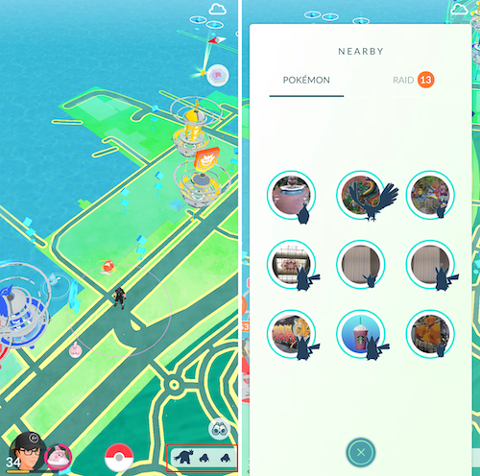
\includegraphics[width=0.8\textwidth]{apki_ss/pokemon.png}
    \caption{Pokemon go}
\end{figure}
Pokemon Go posłużyło jako inspiracja do stworzenia aspektu kolekcjonerskiego w naszej aplikacji, użytkownik może traktować pocztówki jak swego rodzaju pokemony, kolekcjonować je i wymieniać się z znajomymi a przy tym zachęcany jest do aktywnego spędzania czasu poprzez zwiedzanie nowych miejsc w celu zdobycia nowych pocztówek

\newpage
\subsection{Slowly}
Slowly to aplikacja która pozwala użytkownikom na wymianę listów, elementem wyróżniającym ją pośród zwykłych komunikatorów jet to, że listy dochodzą z opóźnieniem zależnym od odległości między komunikującymi się osobami. W momencie wysłania takiego listu użytkownik dostaje powiadomienie o nadchodzącym liście i dacie jego przyjścia, przez co może z niecierpliwością wyczekiwać nowej wiadomości. Aplikacja ta łączy stare z nowoczesnym -- wysyłanie listów z aplikacją społecznościową rozwijając przy tym personalną więź z każdym kolejnym listem. W aplikacji istnieje także możliwość kolekcjonowania znaczków z różnych stron świata i nie tylko, gdy dostaniemy list z takowym znaczkiem automatycznie trafia on do naszej kolekcji.
\begin{figure}[H]
    \centering
    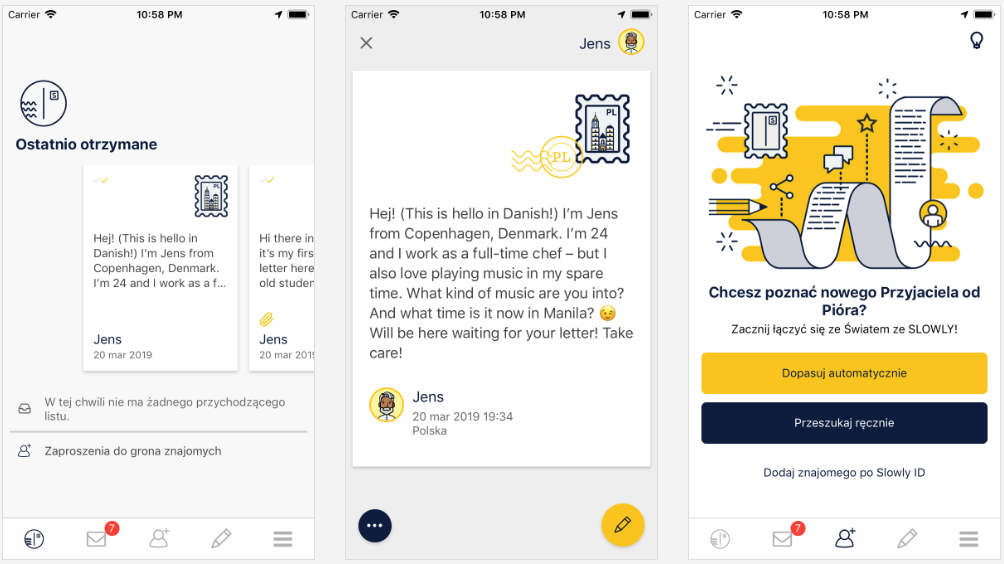
\includegraphics[width=1\textwidth]{apki_ss/slowly.png}
    \caption{Slowly}
\end{figure}
Slowly posłużyło jako inspiracja do części prywatnej aspektu społecznościowego oraz do połączenia czegoś starodawnego i już niezbyt używanego z nowoczesnym sposobem jakim jest aplikacja społecznościowa, tak jak listy w Slowly tak samo pocztówki w naszej aplikacji są kierowane do jednej konkretnej osoby co czyni je wyjątkowymi
\newpage
\subsection{Książeczki PTTK}
Polskie Towarzystwo Turystyczno-Krajoznawcze pozwala na zdobywanie specjalnych pieczątek w przeznaczonych do tego książeczkach. Pieczątki można zbierać między innymi z specjalnie wyznaczonych szlaków turystycznych, gdy jesteśmy w odpowiednim miejscu wystarczy podejść do informacji turystycznej i poprosić o takową pieczątkę. Po zebraniu odpowiedniej ilości konkretnych pieczątek możemy ubiegać się o specjalne odznaki. Rozwiązanie to pozwala na unikatowe dokumentowanie odwiedzonych miejsc oraz nagradza użytkownika za konsekwentne ich zbieranie
\begin{figure}[H]
    \centering
    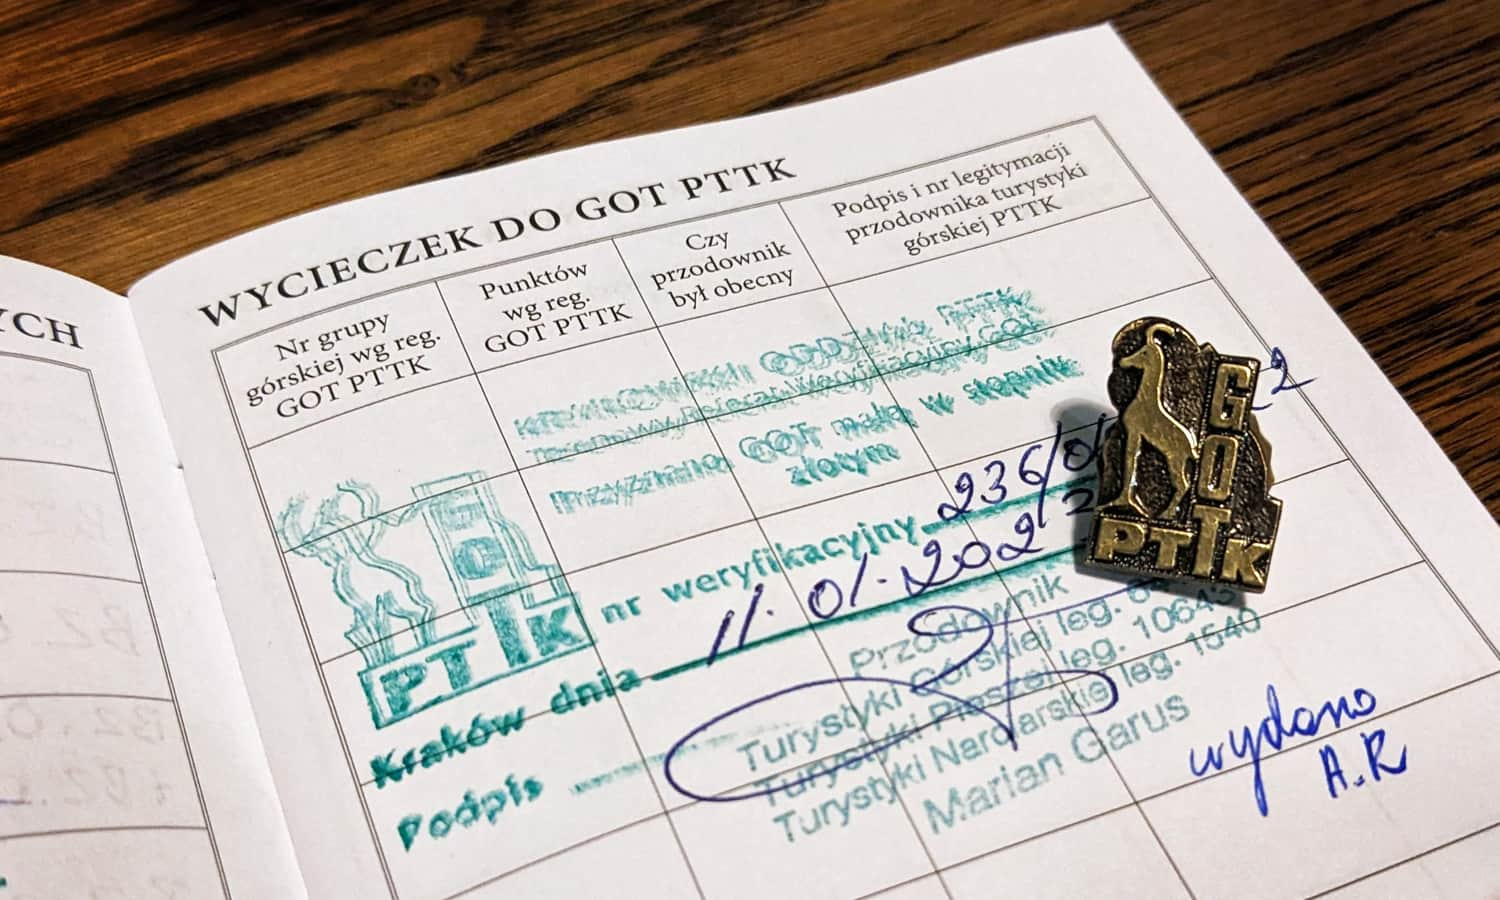
\includegraphics[width=1\textwidth]{apki_ss/pttk.jpg}
    \caption{Książeczka i odznaka PTTK}
\end{figure}

\subsection{Tradycyjne Pocztówki}
Oczywiście nie można nie wspomnieć o rozwiązaniu z świata rzeczywistego są pocztówki, które możemy kupić praktycznie w każdym miejscu na ziemi. Same pocztówki są zazwyczaj bardzo tanie i wysłanie ich również jest możliwe z prawie każdego miejsca na ziemi. Sporą wadą jest to że czas dostarczenia często przekracza kilka tygodni jak nie miesięcy, dodatkowo istnieje spora szansa, że pocztówka zagubi się gdzieś po drodze.

\newpage
\section{Docelowy typ odbiorcy}
Aplikacja jest skierowana do różnorodnej grupy odbiorców i każdy powinien znaleźć w niej aspekt który zaspokoi jego potrzeby, jednak do celu określenia konkretnego docelowego odbiorcy wyróżniamy trzy różne typy:

\begin{itemize}
    \item \textbf{Pasjonat trendów i tradycji} -- Docelowym typem odbiorcy jest osoba która jest na bieżąco z najnowszymi trendami ale nie zaniedbuje również tradycyjnych rozwiązań, aplikacja spełnia oczekiwania takiego użytkownika łącząc tradycyjny zwyczaj wysyłania pocztówek z nowoczesną aplikacją społecznościową. 
    \item \textbf{Miłośnik podróży i kolekcjoner} -- kolejnym docelowym odbiorcą może być osoba dla której podróżowanie to pasja i jednocześnie chce mieć coś w swojej kolekcji z odwiedzonych miejsc. Aplikacja spełnia wymagania takiej osoby ponieważ poprzez zbieranie pocztówek z konkretnych miejsc może dokumentować swoją obecność z danego miejsca jednocześnie poszerzając swoją kolekcję
    \item \textbf{Uniwersalny użytkownik} -- nie ograniczając się do konkretnych grup aplikacja jest odpowiednia dla każdego, dzięki uniwersalnemu tematowi i prostej obsłudze korzystać może z niej każdy, nawet osoba która nie podróżuje może po prostu tylko otrzymywać pocztówki od znajomych
\end{itemize}

\section{Uzasadnienie wyboru}
Na rynku aplikacji oraz w prawdziwym świecie istnieje wiele różnych rozwiązań które w niektórych aspektach pozwalają pomóc rozwiązać postawiony problem, w wielu przypadkach są to rozwiązania które osiągnęły duży sukces. Dlatego inspirując się tymi popularnymi połączyliśmy najważniejsze ich aspekty, aby stworzyć aplikację która pozwoli na ponowny wzrost zainteresowania tak prostą i przyjemną czynnością jaką jest wysyłanie pocztówek. Łącząc tradycję która w ostatnich latach zanika z popularnością aplikacji społecznościowych możemy ponownie przywrócić ten zwyczaj w przystępniejszej formie, nie trzeba już szukać na straganach specjalnych kartek, wystarczy odpalić aplikacje, zebrać pocztówkę oraz wysłać ją wraz z krótką wiadomością do bliskiej nas osoby. Aplikacja pozwala budować specjalne więzi międzyludzkie a przy tym propaguje także aktywne spędzanie wolnego czasu na zwiedzaniu ciekawych miejsc w okolicy jak i na całym świecie.

\newpage

%%%%%%%%%%%%%%%%%%%%%%%%





% TODO
\chapter{Wymagania}
\label{ch:wymagania}

\section{Wymagania funkcjonalne użytkownika wspólne dla aplikacji mobilnej oraz webowej}
\begin{itemize}
    \item Każdy użytkownik może zarejestrować swoje konto przy pomocy adresu e-mail, nazwy użytkownika oraz bezpiecznego hasła.
    \item Każdy użytkownik może uwierzytelnić się za pomocą adresu e-mail oraz hasła.
    \item Każdy użytkownik może zmienić motyw kolorystyczny aplikacji.
    \item Każdy użytkownik może edytować dane swojego profilu który składa się z następujących elementów:
    \begin{itemize}
        \item Zdjęcie tła profilu.
        \item Zdjęcie profilu.
        \item Imię.
        \item Nazwisko.
        \item Datę urodzin.
        \item Kraj zamieszkania.
        \item Krótki opis użytkownika.
        \item Ulubione otrzymane pocztówki.
    \end{itemize}
    \item Każdy użytkownik może zobaczyć swoją kolekcję pocztówek do wysłania.
    \item Każdy użytkownik może zobaczyć swoją kolekcję odebranych pocztówek.
    \item Każdy użytkownik może zobaczyć kolekcję odwiedzonych miejsc.
    \item Każdy użytkownik może zobaczyć wszystkie możliwe miejsca w których można zdobyć pocztówkę.
    \item Każdy użytkownik może wyszukać dowolnego innego użytkownika.
    \item Każdy użytkownik może zobaczyć profil dowolnego innego użytkownika.
    \item Każdy użytkownik może zaobserwować dowolnego innego użytkownika.
    \item Każdy użytkownik może zobaczyć przez jakich innych użytkowników jest obserwowany.
    \item Każdy użytkownik może wysłać pocztówkę, każdemu innemu użytkownikowi. Pocztówka może zawierać informacje takie jak:
    \begin{itemize}
        \item Tytuł
        \item Opis
    \end{itemize}
\end{itemize}
\section{Wymagania funkcjonalne użytkownika wyłączne aplikacji mobilnej}
\begin{itemize}
    \item Każdy użytkownik może zmienić podstawowe ustawienia aplikacji takie jak:
    \begin{itemize}
        \item Ustawienia powiadomień
        \item Promień w którym wyświetlać się będą powiadomienia o dostępnych pocztówkach
        \item Preferowany format daty
        \item Preferowany system miar
    \end{itemize}
    \item Każdy użytkownik może włączyć lokalizowanie pocztówek w okolicy oraz wybrać promień w którym odbywa się lokalizowanie.
    \item Każdy użytkownik powinien otrzymać powiadomienie gdy w pobliżu pojawi się pocztówka do zebrania oraz lokalizowanie pocztówek jest włączone.
    \item Każdy użytkownik może wyświetlić wszystkie pocztówki w ustalonym wcześniej obrębie względem swojej lokalizacji.
    \item Każdy użytkownik może wyświetlić oraz odebrać dowolną możliwą do zebrania pocztówkę w ustalonym wcześniej obrębie względem aktualnej lokalizacji.
    \item Aplikacja podczas wczytywania danych z aplikacji serwerowej powinna pokazywać wstępny układ stron za pomocą migoczących paneli.
\end{itemize}

\section{Wymagania niefunkcjonalne użytkownika dla aplikacji mobilnej}
\begin{itemize}
    \item Aplikacja powinna działać poprawnie na dowolnym telefonie z systemem Android X.X+.
    \item Aplikacja powinna pozwalać na poprawne działanie tylko w przypadku połączenia z aplikacją serwerową.
    \item Aplikacja powinna pozwalać na odbieranie pocztówek tylko gdy lokalizacja jest włączona.
\end{itemize}

\section{Wymagania niefunkcjonalne użytkownika dla aplikacji webowej}
\begin{itemize}
    \item Aplikacja powinna działać poprawnie na dowolnej przeglądarce internetowej.
    \item Aplikacja powinna pozwalać na poprawne działanie tylko w przypadku połączenia z aplikacją serwerową.
\end{itemize}

\section{Wymagania niefunkcjonalne użytkownika dla aplikacji serwerowej}
\begin{itemize}
    \item Czas odpowiedzi aplikacji serwerowej powinien być mniejszy niż 1s dla większości operacji.
    \item Wszystkie dane wrażliwe użytkowników znajdujące się w bazie danych powinny być odpowiednio zabezpieczone przed nieautoryzowanym dostępem.
    \item Hasła użytkowników powinny być szyfrowane za pomocą algorytmu PBKDF2 z pseudolosową funkcją -- HMAC-SHA-1.
    \item Komunikacja między aplikacją serwerową a pozostałymi używanymi aplikacjami powinna odbywać się przy użyciu bezpiecznego protokołu HTTPS.
    \item Aplikacja serwerowa powinna być zgodna z najnowszymi standardami bezpieczeństwa OWASP Top 10 oraz spełniać wymogi dotyczące ochrony danych osobowych.
\end{itemize}



%%%%%%%%%%%%%%%%%%%%%
%% RYSUNEK Z PLIKU
%
%\begin{figure}
%\centering
%
\includegraphics[width=0.5\textwidth]{./politechnika_sl_logo_bw_pion_pl.pdf}
%\caption{Podpis rysunku zawsze pod rysunkiem.}
%\label{fig:etykieta-rysunku}
%\end{figure}
%Rys. \ref{fig:etykieta-rysunku} przestawia …
%%%%%%%%%%%%%%%%%%%%%
%
%%%%%%%%%%%%%%%%%%%%%
%% WIELE RYSUNKÓW 
%
%\begin{figure}
%\centering
%\begin{subfigure}{0.4\textwidth}
%    
\includegraphics[width=\textwidth]{./politechnika_sl_logo_bw_pion_pl.pdf}
%    \caption{Lewy górny rysunek.}
%    \label{fig:lewy-gorny}
%\end{subfigure}
%\hfill
%\begin{subfigure}{0.4\textwidth}
%    
\includegraphics[width=\textwidth]{./politechnika_sl_logo_bw_pion_pl.pdf}
%    \caption{Prawy górny rysunek.}
%    \label{fig:prawy-gorny}
%\end{subfigure}
%
%\begin{subfigure}{0.4\textwidth}
%    
\includegraphics[width=\textwidth]{./politechnika_sl_logo_bw_pion_pl.pdf}
%    \caption{Lewy dolny rysunek.}
%    \label{fig:lewy-dolny}
%\end{subfigure}
%\hfill
%\begin{subfigure}{0.4\textwidth}
%    
\includegraphics[width=\textwidth]{./politechnika_sl_logo_bw_pion_pl.pdf}
%    \caption{Prawy dolny rysunek.}
%    \label{fig:prawy-dolny}
%\end{subfigure}
%        
%\caption{Wspólny podpis kilku rysunków.}
%\label{fig:wiele-rysunkow}
%\end{figure}
%Rys. \ref{fig:wiele-rysunkow} przestawia wiele ważnych informacji, np. rys. \ref{fig:prawy-gorny} jest na prawo u góry.
%%%%%%%%%%%%%%%%%%%%%



\chapter{Metodyka pracy nad projektowaniem i implementacją}
\label{ch:Metodyka}

\section{Opis użytych narzędzi}

\begin{itemize}
    \item \textbf{Visual Studio (IDE)} -- zintegrowane środowisko programistyczne stworzone przez firmę Microsoft. Oferuje narzędzia dla wielu języków programowania w tym dla wykorzystanego w przypadku naszej aplikacji serwerowej C\#.
    \item \textbf{SQL Server Management Studio} -- zintegrowane środowisko bazy danych do jej obsługi, które zawiera wszystkie potrzebne funkcjonalności. 
    \item \textbf{Visual Studio Code} -- prosty i elastyczny edytor kodu posiadający wsparcie dla wielu języków programowania oraz obszerne wsparcie dla wszelakich dodatków.
    \item \textbf{Android Studio} -- zintegrowane środowisko programistyczne stworzone przez firmę Google do tworzenia aplikacji mobilnych, narzędzie to zawiera wbudowany emulator systemów android który pozwala na proste testowanie aplikacji. Samo środowisko pozwala na obsługę frameworku Flutter który został wykorzystany do stworzenia aplikacji mobilnej.
    \item \textbf{Miro} -- platforma online służąca do tworzenia diagramów, map myśli czy prototypów i koncepcji. Platforma pozwala na pracę nad projektem w czasie rzeczywistym wielu osobom co okazało się przydatne podczas początkowej fazy projektowania aplikacji.
    \item \textbf{Figma} -- platforma do projektowania interfejsów użytkownika, pozwala ona tworzyć interaktywne prototypy na przykład aplikacji mobilnych, ponadto pozwala na pracę zespołową w czasie rzeczywistym i jest dostępna z poziomu przeglądarki internetowej.
    \item \textbf{dbdiagram.io} -- narzędzie dostępne w przeglądarce służące do projektowania relacyjnych baz danych za pomocą wizualnego edytora, samo narzędzie pozwala także na automatyczne generowanie kodu SQL
    \item \textbf{Github} -- To platforma internetowa która służy do zarządzania projektami przy użyciu systemu kontroli wersji Git. Platforma ta pozwala na łatwą współpracę podczas pracy nad kodem, śledzenie historii zmian, zarządzanie problemami czy tworzenie specjalnych gałęzi. Github jest powszechnie używany na całym świecie przy tworzeniu projektów open-source a także w firmach do prywatnych repozytoriów kodu.
    \item \textbf{Github Desktop/Github Kraken} -- narzędzia pozwalające na zarządzanie repozytoriami Git w sposób graficzny, narzędzia te oferują funkcjonalności takie jak przeglądanie historii commitów, klonowanie repozytoriów, tworzenie gałęzi, synchronizacja z repozytorium zdalnym czy po prostu commitowanie zmian.
    \item \textbf{Discord} -- platforma komunikacyjna dostępna z poziomu przeglądarki lub aplikacji, początkowo zaprojektowana dla społeczności graczy szybko rozszerzyła swoje zastosowanie dla wszelakich innych grup społecznych. Platforma umożliwia tworzenie serwerów na których użytkownicy mogą komunikować się ze sobą na wiele sposobów między innymi poprzez kanały głosowe. Discord pozwala również na wysyłanie wiadomości tekstowych oraz plików, to wszystko sprawia umożliwia łatwą i przyjemną komunikację międzyludzką w czasie rzeczywistym
\end{itemize}
\newpage

\section{Wczesne Etapy Projektowania}

W najwcześniejszym etapie projektowania aplikacji został wymyślony główny koncept czyli na czym ma polegać cała aplikacja, co ma sobą reprezentować oraz do kogo ma być skierowana. Narzędziem, które w tym pomogło było Miro w bezproblemowo została stworzona mapa myśli przedstawiająca parę różnych pomysłów, lecz wszystkich zgodnych co do jednego, aplikacja powinna zrzeszać jakąś społeczność i pozwalać w nowoczesny sposób aktywnie spędzać czas, ostatecznie zostały wybrane dwa dosyć podobne pomysły
aplikacja społecznościowa do zbierania wirtualnych magnesów oraz aplikacja społecznościowa do zbierania i przesyłania wirtualnych pocztówek. Finalnie zatwierdzony został pomysł z zbieraniem wirtualnych pocztówek, gdzie początkowo aplikacja webowa miała istnieć tylko na zasadzie wizytówki lecz z czasem pomysł ewoluawał na tyle że część funkcjonalności została tam również zaimplementowana.
\begin{figure}[H]
    \centering
    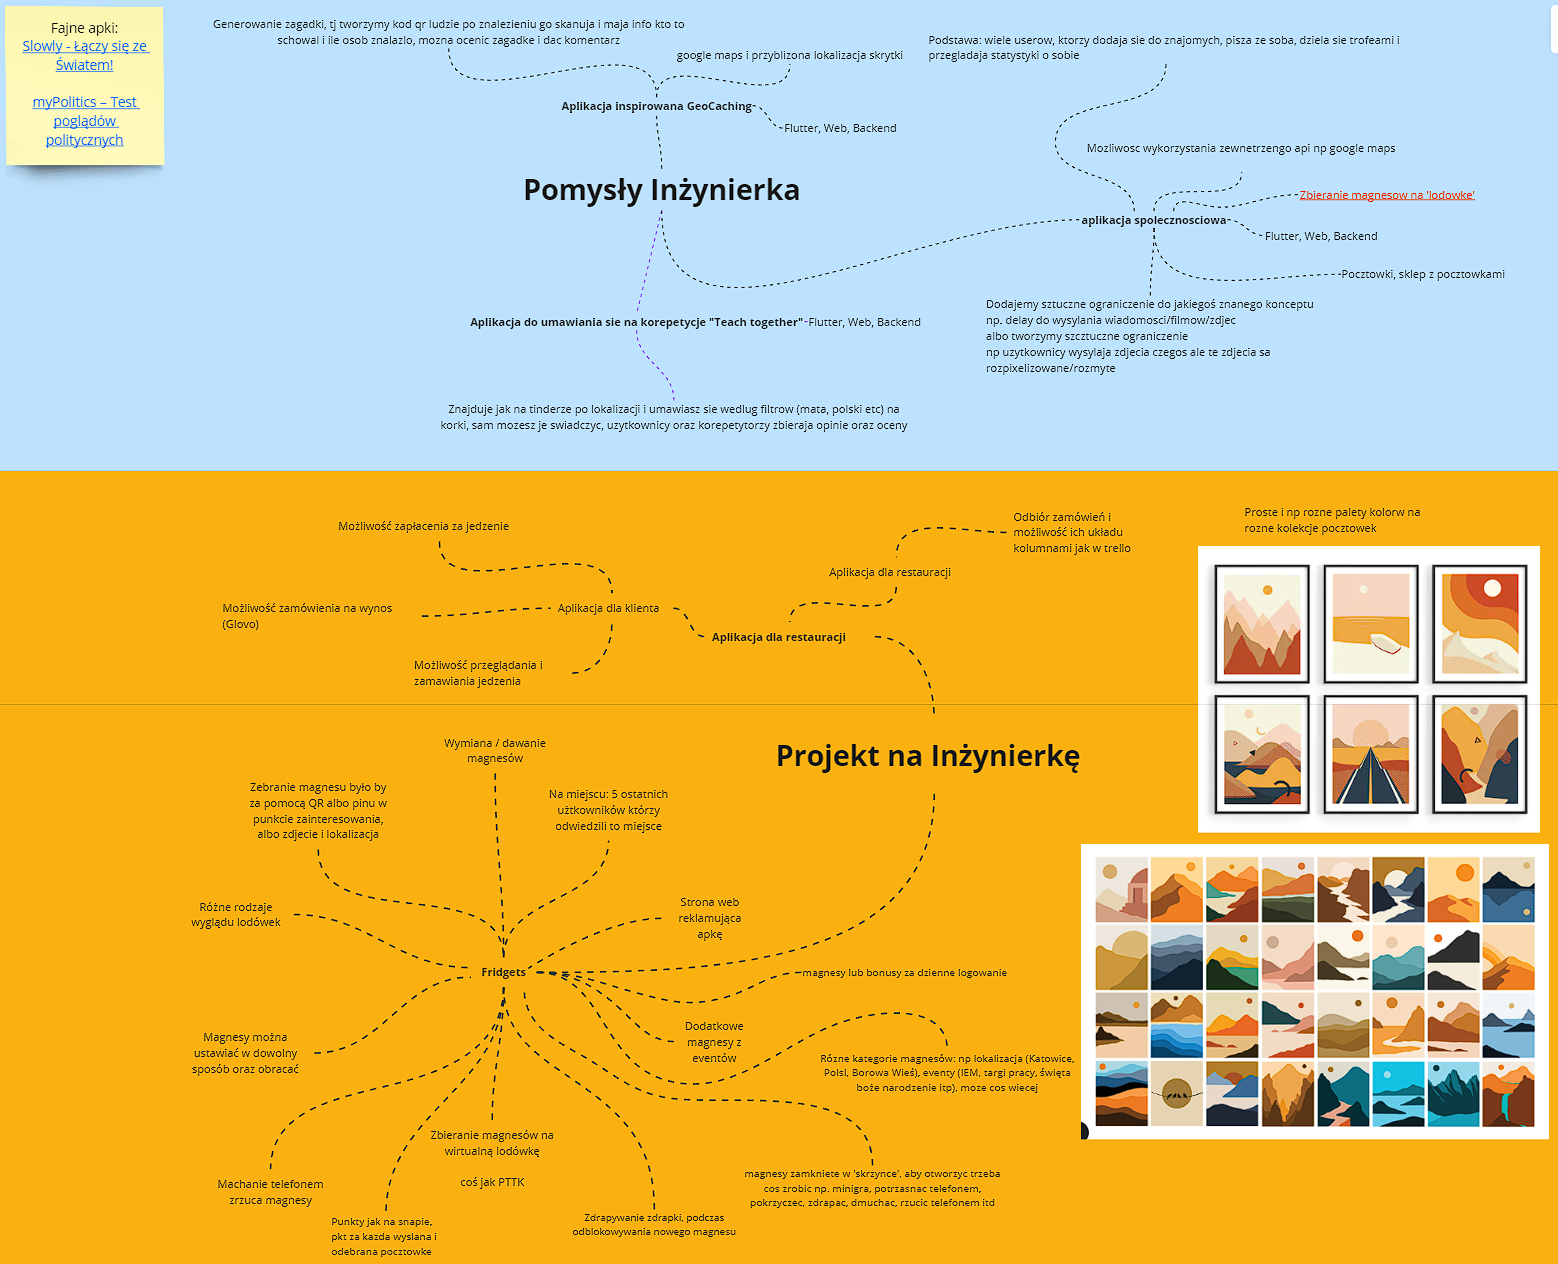
\includegraphics[width=1\textwidth]{wizje_ss/miro.png}
    \caption{Miro - mapa myśli pomysłów na aplikację}
\end{figure}
\newpage

Kolejnym etapem wczesnego projektowania było wybranie odpowiedniej palety kolorów oraz ustalenie wstępnego designu aplikacji, jako że głównym trzonem aplikacji miała być aplikacja mobilna to właśnie na nią została przeznaczona największa ilość czasu w tym etapie projektowania. W celu wykonania tego zadania bardzo pomogło narzędzie Figma, w którym przetestowane zostały różne koncepcje oraz warianty kolorystyczne do aplikacji mobilnej oraz aplikacji webowej. Warto zaznaczyć, że także na tym etapie po wielu propozycjach została wybrana nazwa całej aplikacji -- Postcardia.
\begin{figure}[H]
    \centering
    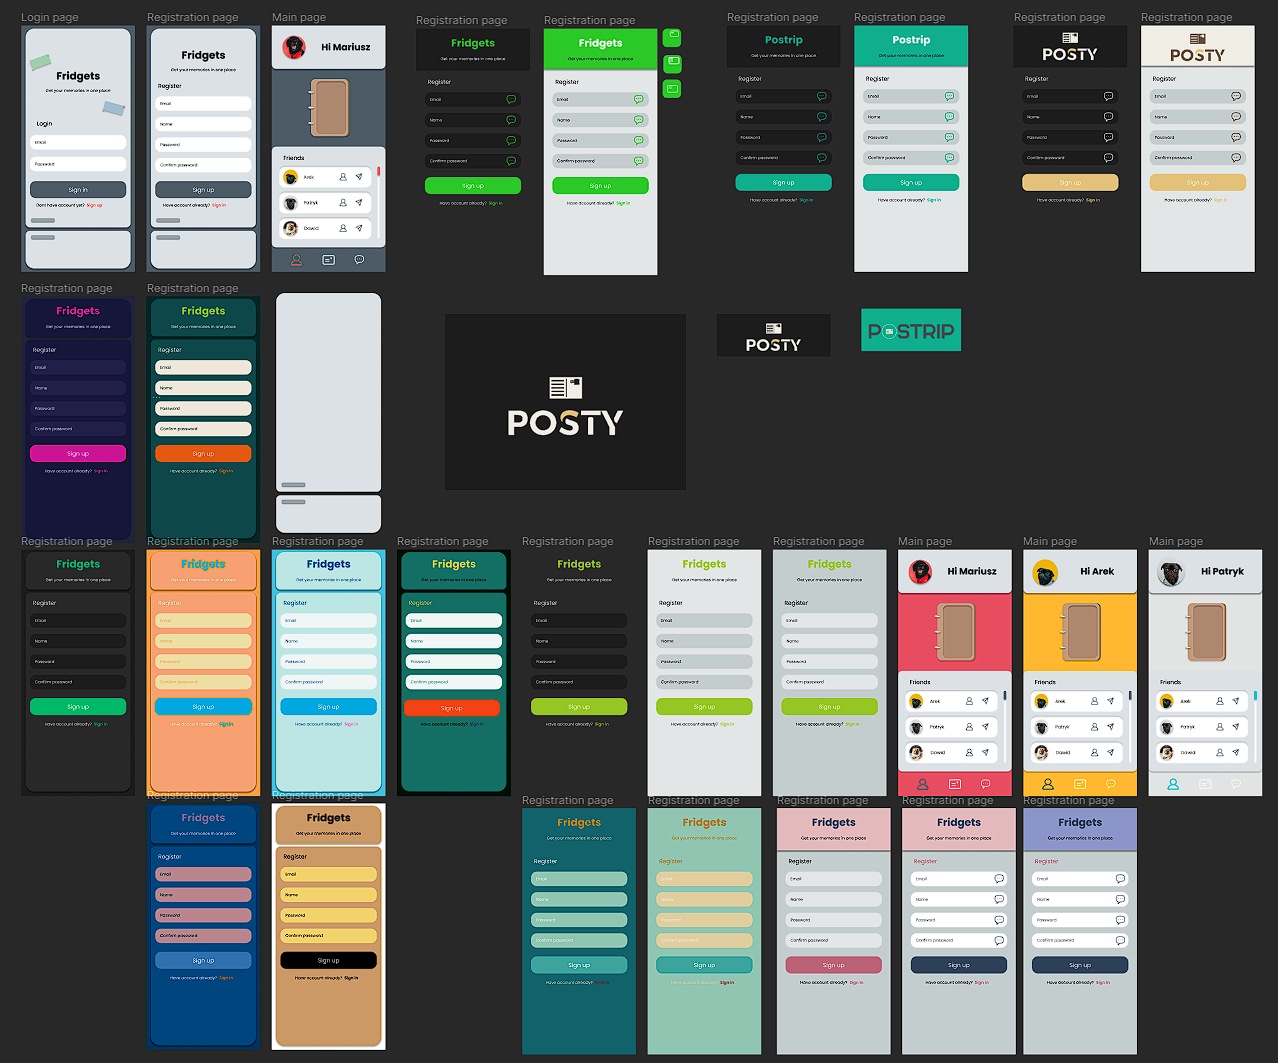
\includegraphics[width=1\textwidth]{wizje_ss/figma-colors.png}
    \caption{Próby znalezienia odpowiedniej palety kolorów do projektu oraz nazwy}
\end{figure}
\newpage

\begin{figure}[H]
    \centering
    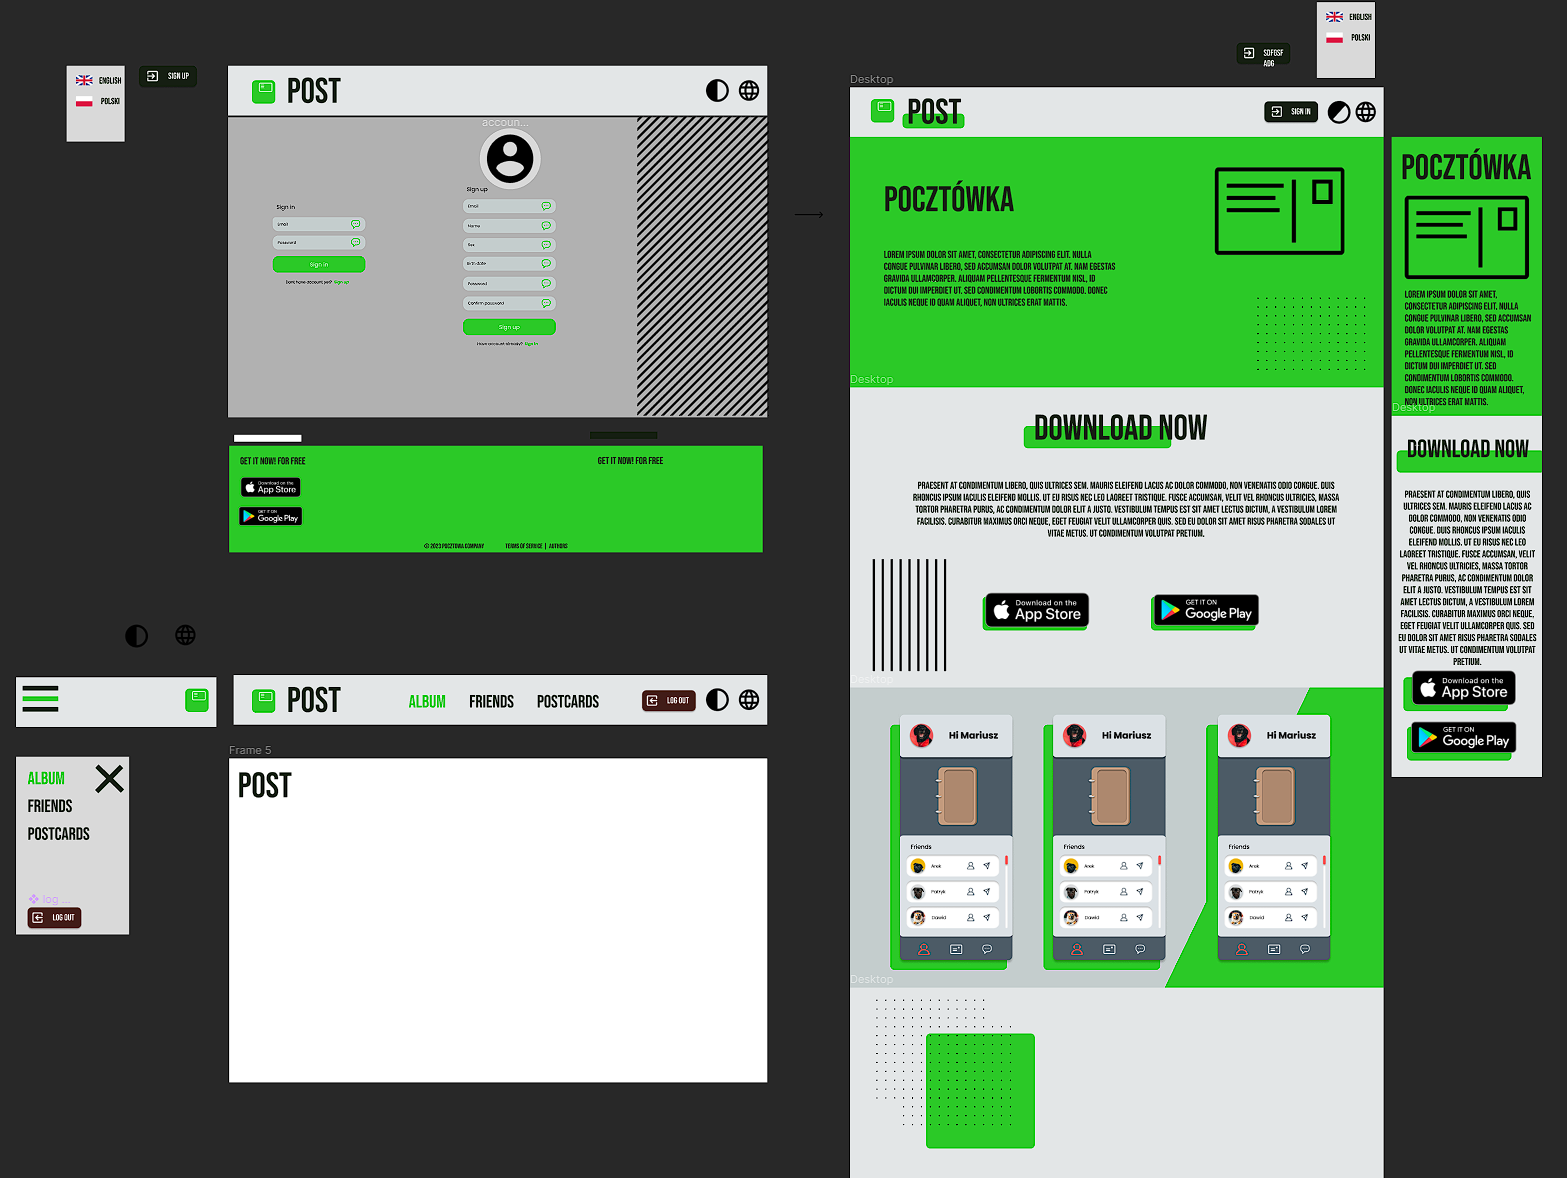
\includegraphics[width=0.9\textwidth]{wizje_ss/figma-web-green.png}
    \caption{Wstępny design aplikacji webowej}
\end{figure}
\begin{figure}[H]
    \centering
    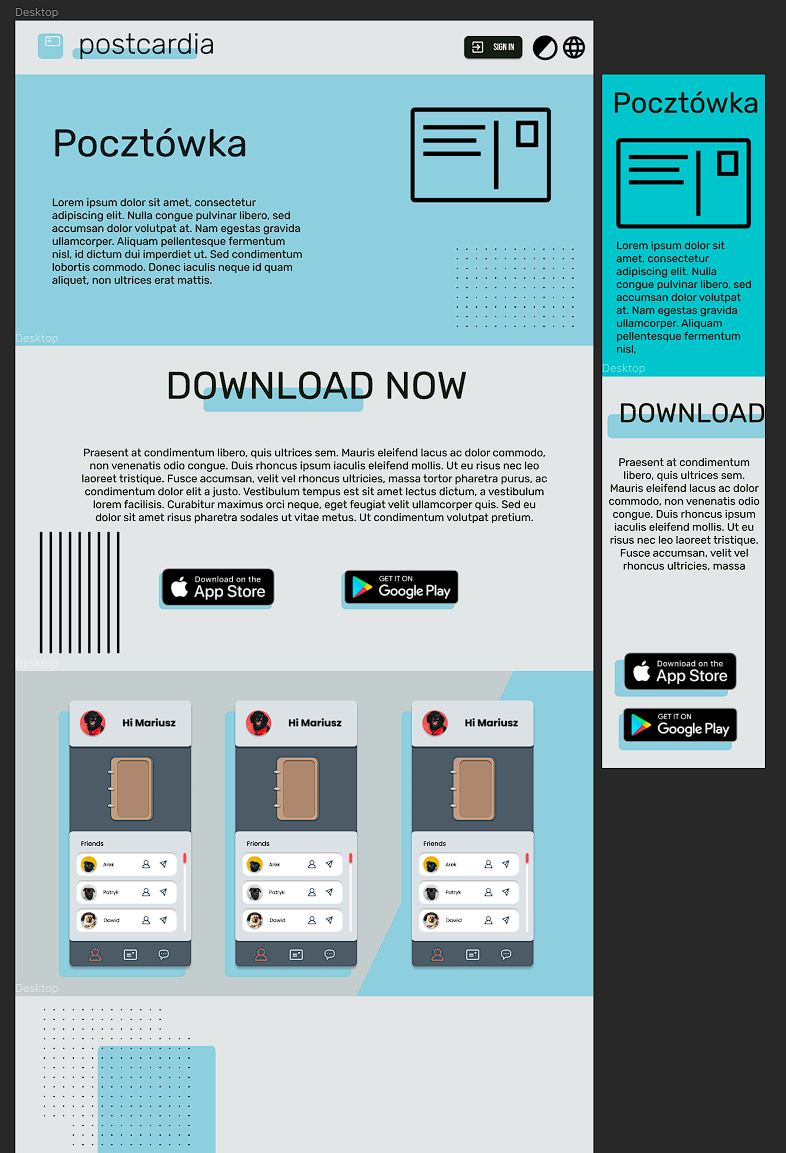
\includegraphics[width=0.45\textwidth]{wizje_ss/figma-web-blue.png}
    \caption{Aplikacja webowa z inną paletą kolorów}
\end{figure}
\newpage

Podczas ostatniego etapu wstępnego projektowania części wizualnej został stworzony wstępny widok większości stron w aplikacji mobilnej, celem samego projektowania nie było stworzenie finalnego, mocno wiążącego designu, lecz stworzenie inspiracji i pomocnej wizualizacji dla programistów zajmujących się aplikacją mobilną.

Podczas tworzenia wstępnego designu priorytetem było skupienie się na stworzeniu przejrzystego i przyjaznego środowiska dla użytkownika które zarazem jest funkcjonalne i estetyczne. Sam użytkownik docelowo powinien intuicyjnie przemieszczać się po wszystkich zakładkach oraz od razu wiedzieć gdzie znajduje się jaka funkcjonalność aplikacji.

W rezultacie wizualizacja mocno pomogła w procesie tworzenia aplikacji mobilnej a stworzony design finalnie nie odbiega mocno od designu zaimplementowanego w właściwej aplikacji, wiele elementów jak i koncepcji jest niemalże identycznych.



\begin{figure}[H]
    \centering
    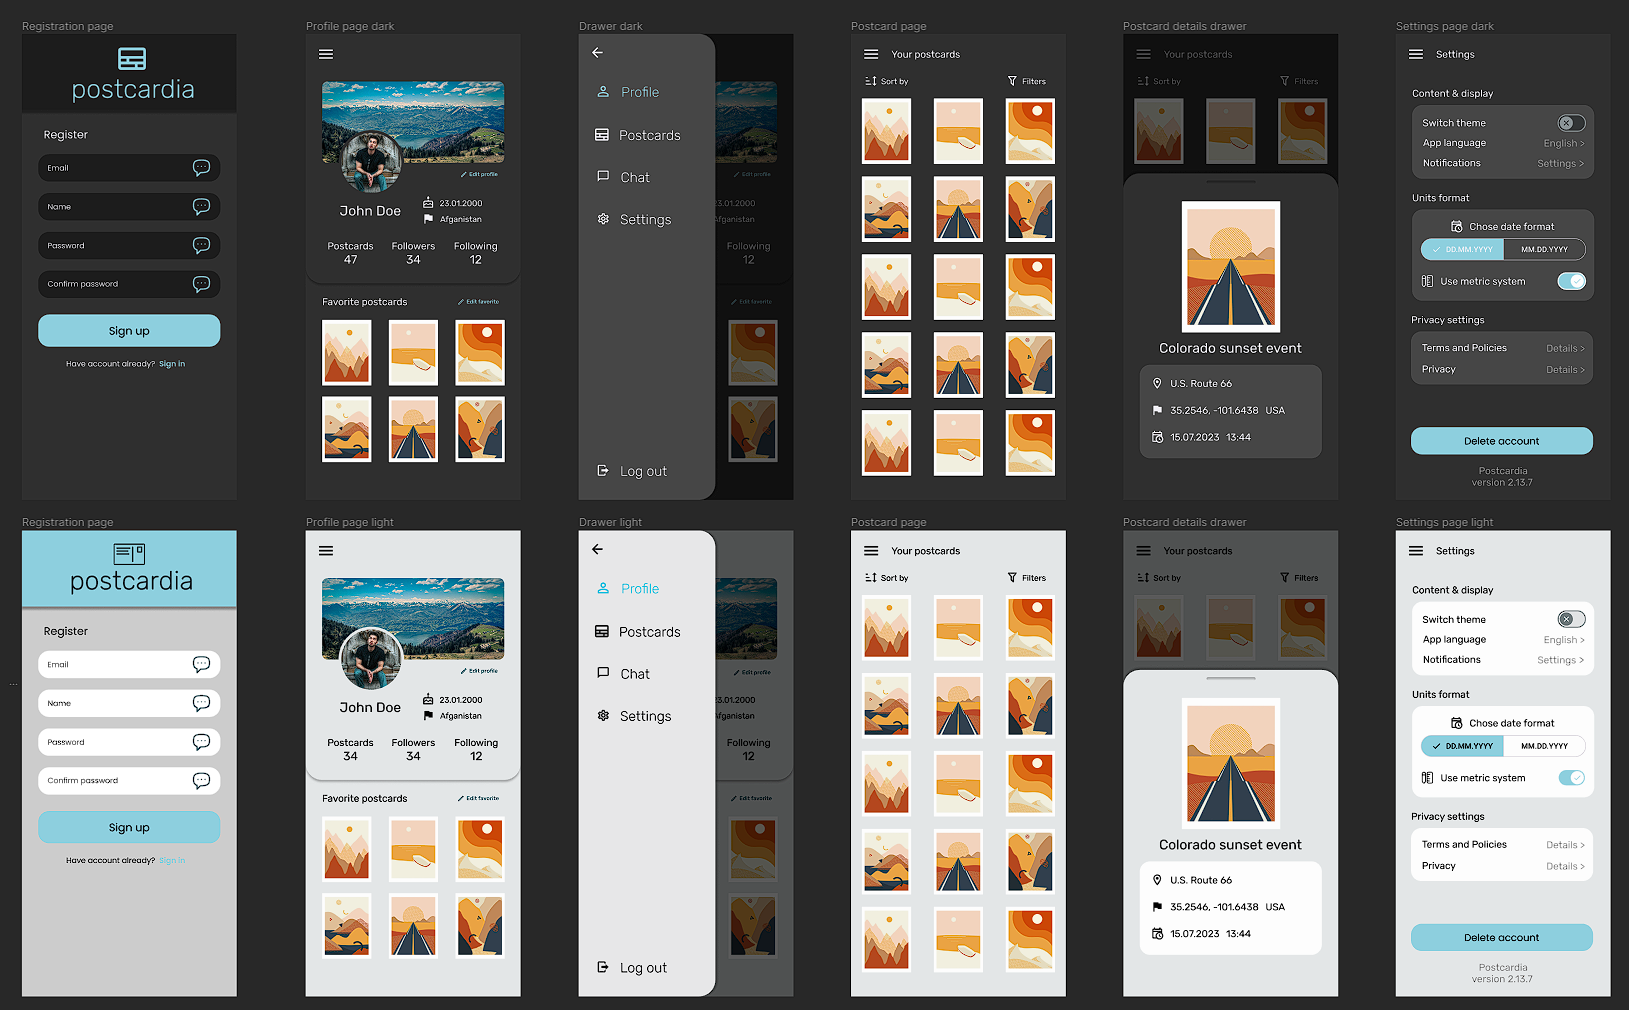
\includegraphics[width=1\textwidth]{wizje_ss/figma-designs.png}
    \caption{Wstępnie wybrany design aplikacji mobilnej}
\end{figure}
\newpage
Warto zaznaczyć, że podczas wstępnego projektowania został stworzony także wstępny model bazy danych określający poszczególne tabele i relacje, baza danych finalnie została trochę zmodyfikowana, lecz etap ten pozwolił wstępnie oszacować wielkość oraz złożoność finalnej bazy danych a także pozwolił przemyśleć pewne rozwiązania i delikatnie je zmodyfikować.
\begin{figure}[H]
    \centering
    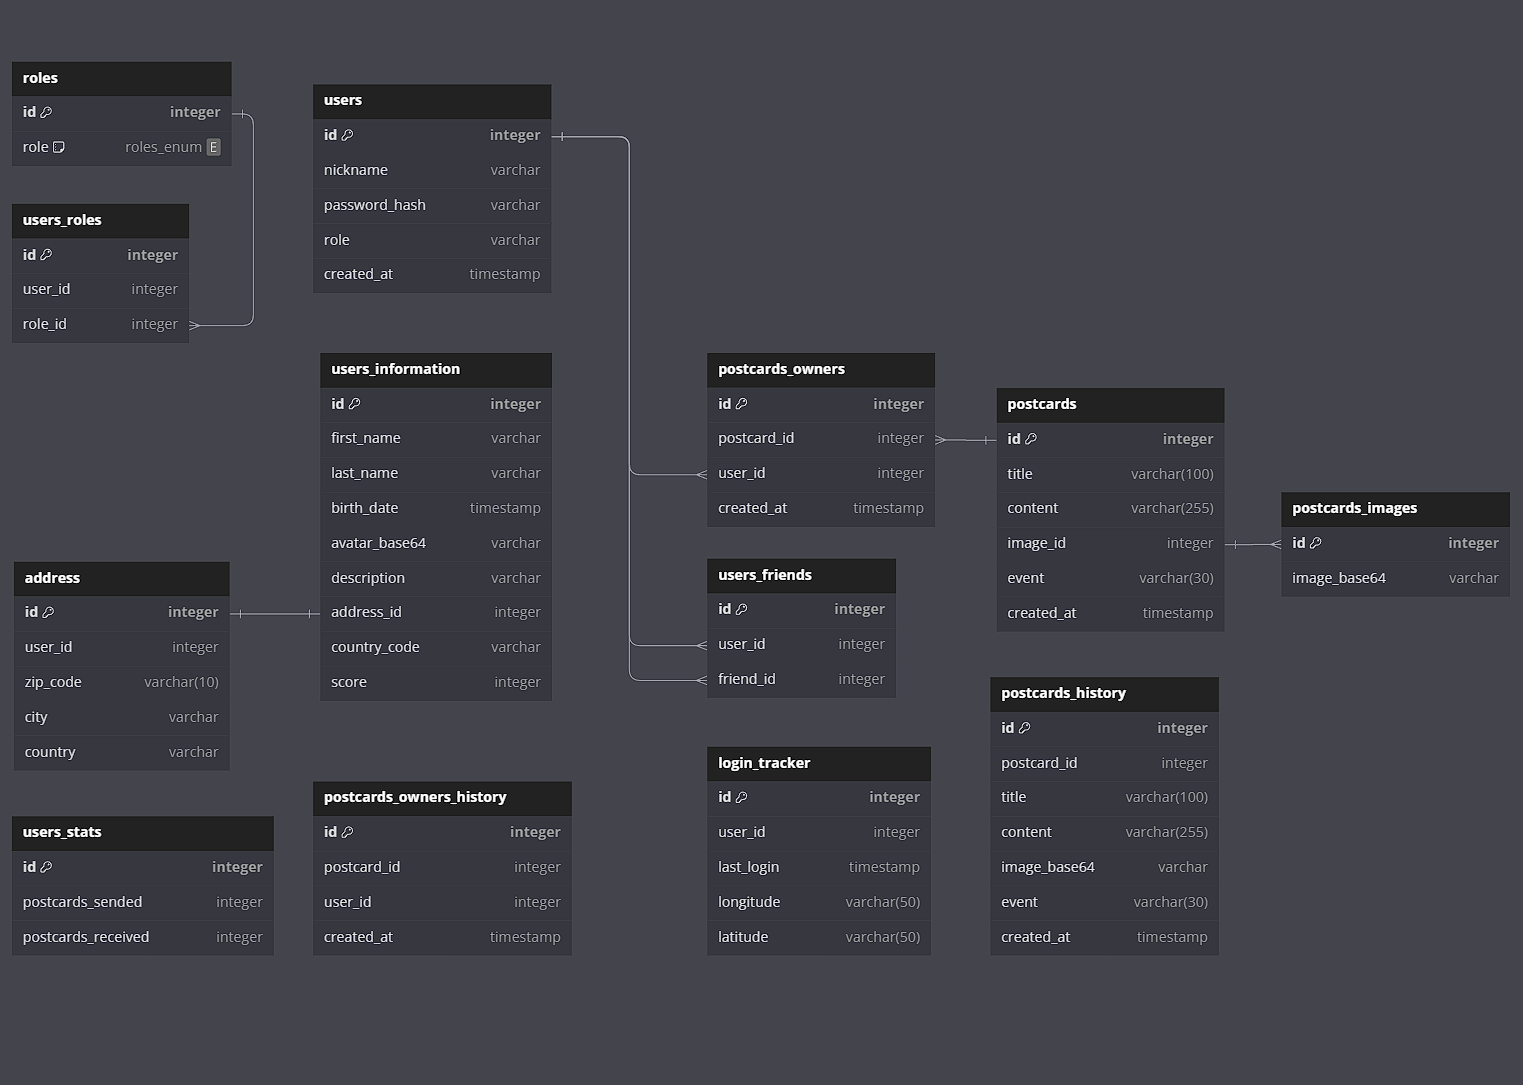
\includegraphics[width=1\textwidth]{wizje_ss/baza.png}
    \caption{Wstępnie wybrany design aplikacji mobilnej}
\end{figure}
\newpage

\section{System kontroli wersji}
Podczas fazy implementacji projektu niezbędny okazał się system kontroli wersji git - narzędzie które pozwala między innymi na:
\begin{itemize}
    \item Kontrolę wersji -- śledzenie wszystkich ważnych zmian w projekcie.
    \item Łatwą współpracę programistyczną -- równoczesne edytowanie tych samych plików poprzez różne osoby.
    \item Rozgałęzianie i scalanie -- tworzenie specjalnych gałęzi projektu do równoczesnej pracy nad różnymi funkcjonalnościami aplikacji.
    \item Podgląd zmian -- Automatyczny wyświetlanie dodanych, zmienionych i usuniętych plików czy linii kodu.
    \item Śledzenie autorskiej historii -- Każda zmiana jest przypisana do użytkownika który ją stworzył.
    \item Używanie lokalnego repozytorium -- możliwość pracy offline z późniejszą opcją synchronizacji z repozytorium zdalnym.
    \item Cofanie zmian -- możliwość powrotu do dowolnego wcześniejszego stanu projektu.
\end{itemize}
Sam system kontroli wersji ściśle współpracuje z platformą GitHub na której została stworzona specjalna organizacja na potrzeby tworzenia aplikacji. W organizacji tej znajduje się pięć różnych repozytoriów:
\begin{enumerate}
    \item Repozytorium dla dokumentacji projektu.
    \item Repozytorium dla aplikacji serwerowej.
    \item Repozytorium dla aplikacji webowej.
    \item Repozytorium dla aplikacji mobilnej.
    \item *Repozytorium dla starej aplikacji webowej.
\end{enumerate}
*Początkowo aplikacja webowa miała powstać w technologii angular, lecz po wstępnej analizie tematu zdecydowaliśmy się na technologię React w zespół posiadał większe doświadczenie oraz wiedzę
\begin{figure}[H]
    \centering
    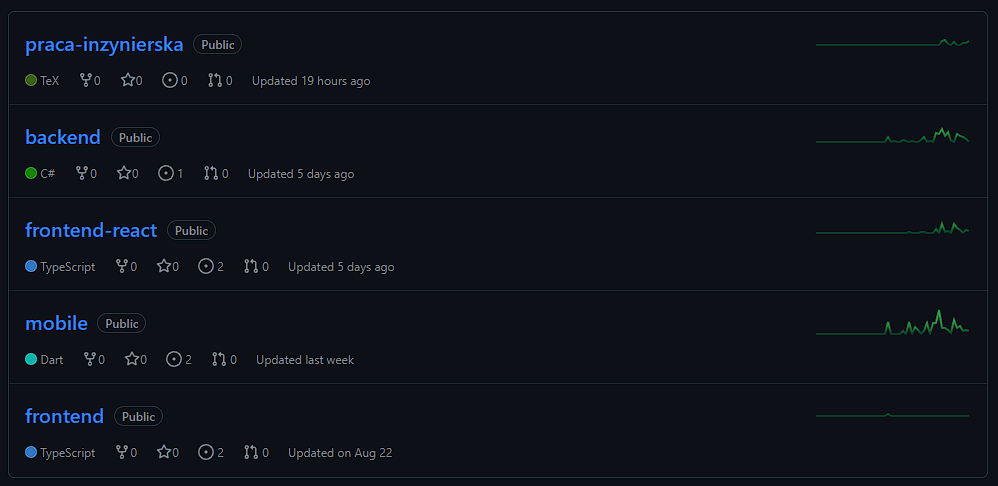
\includegraphics[width=1\textwidth]{github_ss/organizacja.png}
    \caption{Repozytoria w organizacji na platformie GitHub}
\end{figure}


\section{Komunikacja w zespole oraz przydział zadań}
Ważnym aspektem implementacji jak i projektowania była sama komunikacja między członkami zespołu. Jako główną platformę komunikacyjną wybraliśmy aplikację Discord na której konsekwentnie uskuteczniana była metodyka Scrum -- metodyka w której zespół regularnie w cotygodniowych odstępach spotykał się na kanale głosowym aby omówić postęp pracy, zaplanować oraz przydzielić kolejne zadania i w razie potrzeby przedyskutować opóźnienia lub napotkane problemy.

Zadania były tworzone na podstawie brakujących funkcjonalności lub powstałych błędów wymagających poprawek, w tym celu została wykorzystana funkcjonalność Issues z platformy GitHub, funkcjonalność ta pozwala tworzyć konkretne problemy i zadania z możliwością przypisania osoby odpowiedzialnej za wykonanie tego zadania. Narzędzie podczas tworzenia takiego problemu lub zadania daje nam możliwość stworzenia specjalnej gałęzi przeznaczonej dla tego problemu lub zadania dzięki czemu można w łatwy sposób kontrolować postęp prac oraz bezproblemowo działać na projekcie w kilka osób

\begin{figure}[H]
    \centering
    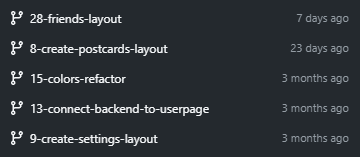
\includegraphics[width=0.5\textwidth]{github_ss/branche.png}
    \caption{Przykładowe gałęzie stworzone na podstawie konkretnego problemu}
\end{figure}
\newpage

Sama platforma GitHub pozwala także na łatwe śledzenie ogólnej aktywności na danych repozytoriach dzięki temu podczas cotygodniowych spotkań bez głębszego analizowania zmienionego kodu i plików można dowiedzieć się o intensywności prac prowadzonych przez inne osoby w projekcie i nie tylko.
\begin{figure}[H]
    \centering
    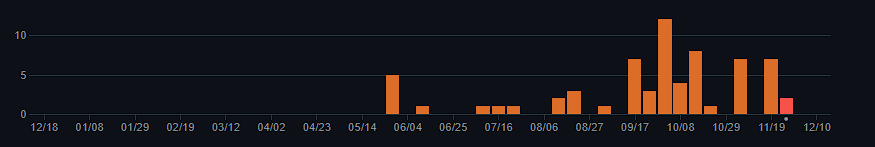
\includegraphics[width=1\textwidth]{github_ss/backend.png}
    \caption{Historia commitów w aplikacji serwerowej}
\end{figure}
\begin{figure}[H]
    \centering
    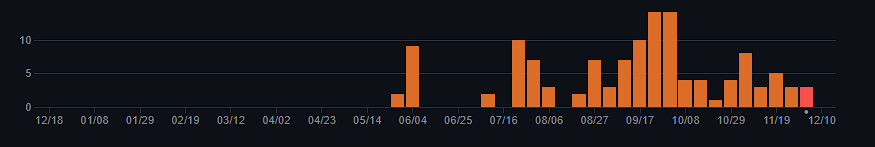
\includegraphics[width=1\textwidth]{github_ss/mobile.png}
    \caption{Historia commitów w aplikacji mobilnej}
\end{figure}
\begin{figure}[H]
    \centering
    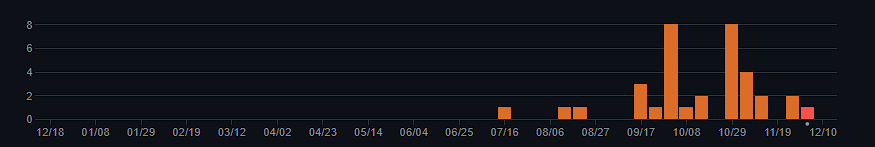
\includegraphics[width=1\textwidth]{github_ss/front.png}
    \caption{Historia commitów w aplikacji webowej}
\end{figure}
 


% TODO
\chapter{Aplikacja mobilna}
\label{ch:05}

% % % % % % % % % % % % % % % % % % % % % % % % % % % % % % % % % % % 
% Pakiet minted wymaga importu: \usepackage{minted}                 %
% i specjalnego kompilowania:                                       %
% pdflatex -shell-escape main                                       %
% % % % % % % % % % % % % % % % % % % % % % % % % % % % % % % % % % % 

%\begin{figure}
%\centering
%\begin{minted}[linenos,frame=lines]{c++}
%class test : public basic
%{
%    public:
%      test (int a);
%      friend std::ostream operator<<(std::ostream & s, 
%                                     const test & t);
%    protected:
%      int _a;  
%      
%};
%\end{minted}
%\caption{Pseudokod w \texttt{minted}.}
%\label{fig:pseudokod:minted}
%\end{figure}




\section{Biblioteki}
W rozdziale tym zostaną omówione biblioteki użyte w projekcie. Na początku omówimy główne biblioteki każdego z modułów. W dalszych podrozdziałach omówimy biblioteki dodatkowe, które wchodzą w skład modułów dodając do nich nowe funkcjonalności lub rozwijając już te istniejące.
\subsection{Biblioteka główna mobilna}
\begin{itemize}
    \item Flutter - jest to technologia stworzona przez firmę Google pozwalająca na tworzenie aplikacji na urządzenia z systemami Android jak i iOS używając tego samego kodu. Językiem wykorzystywanym podczas tworzenia tych aplikacji jest Dart, który również został stworzony przez Google. Napisane we Flutterze aplikacje mobilne wyglądają i działają niemal identycznie na obu systemach z wydajnością, która jest bardzo zbliżona do aplikacji natywnych. Fluttera tworzą dwa podstawowe elementy którymi są framework, który jest niezbędny do poprawnego działania aplikacji oraz pakiet SDK, który jest konieczny do ich tworzenia.
\end{itemize}
\subsection{Biblioteki mobilne dodatkowe}
\begin{itemize}
    \item intl - umożliwia stworzenie pliku zawierającego wszystkie wiadomości zawierające się w aplikacji oraz używanie odpowiednich plików z językami w zależności od ustawień.
    \item http - jest to biblioteka umożliwiająca komunikację pomiędzy aplikacją a serwerem przy użyciu żądań HTTP.
    \item flutter\_bloc - biblioteka, która zawiera w sobie widgety, ułatwiająca wprowadzenie BLoC jako state management w aplikacji.
    \item flutter\_secure\_storage - w aplikacji używany jest do przechowywania JWT otrzymanego podczas logowania. Biblioteka szyfruje wartości jakie otrzymuje przed umieszczeniem ich w pamięci. Na platformie Android jest używane do tego szyfrowanie AES, natomiast na platformie iOS jest to KeyChain. 
    \item jwt\_decoder - jest biblioteka do dekodowania JWT. Dzięki niej możemy sprawdzić, czy token wygasł i na podstawie tego przekierować użytkownika na odpowiednią podstronę.
    \item shimmer - biblioteka dodająca widget używany podczas ładowania danych z serwera.
    \item image\_picker - oficjalna biblioteka umożliwiająca wybieranie zdjęć z galerii lub tworzenie od razu nowych i dalsze ich wykorzystywanie w aplikacji.
    \item country\_picker - biblioteka dodająca widget do wybierania kraju.
    \item auto\_size\_text - jest to biblioteka dająca większą kontrolę nad wyświetlanym tekstem. Dzięki niej łatwo możemy skalować tekst na mniejszych ekranach lub ustawiać limit wierszy przy zawijaniu.
    \item background\_locator\_2 - jest to jedna z istotniejszych bibliotek w naszej aplikacji. Służy ona na do pobierania z telefonu koordynatów. Funkcja kontynuuje działanie, nawet gdy aplikacja działa w tle lub gdy jest całkowicie wyłączona. Biblioteka jest również rozwinięta o funkcje callback, która jest wykonywana za każdym razem gdy pobierane są nowe koordynaty co umożliwia nam wykonywanie wtedy innych funkcji, nawet gdy aplikacja jest wyłączona.
    \item path\_provider - biblioteka wykorzystywana do lokalizowanie plików w systemie.
    \item location\_permissions - umożliwia pobieranie lokalizacji z urządzenia. 
    \item permission\_handler - biblioteka, która obsługuje nadawanie oraz sprawdzanie istniejących zgód na wykorzystywanie poszczególnych serwisów w urządzeniu, takich jak powiadomienia lub pamięć. 
    \item geolocator - biblioteka, która pozwala na komunikację z serwisem odpowiedzialnym za lokalizację. W projekcie jest wykorzystywana w celu sprawdzenia czy lokalizacja jest ciągle włączona na urządzeniu. 
    \item cached\_memory\_image - biblioteka umożliwiająca zapisywanie grafik w pamięci telefonu co eliminuje miganie obrazów podczas ich ciągłego pobierania.
    \item url\_launcher - umożliwia otwieranie linków w osobnej karcie przeglądarki na użądzeniach mobilnych. 
    \item loading\_animation\_widget - biblioteka zawierająca animacje ładowania.
    \item flutter\_animate - biblioteka umożliwiająca animowania dowolnego widgetu w aplikacji.
    \item easy\_debounce - biblioteka upraszczająca oryginalny zapis debouncera języka Dart. 
    \item shared\_preferences - służy do zapisywania różnych zmiennych w pamięci telefonu jako pary klucz-wartość w podobny sposób jak to robi secure storage. 
    \item app\_settings - umożliwia otworzenie ustawień telefonu z poziomu aplikacji.
    \item provider - jest to biblioteka do zarządzania stanem aplikacji. Umożliwia na przebudowanie widoku gdy Consumer wykryje zmianę wartości zmiennej.
    \item flutter\_local\_notifications - biblioteka umożliwiająca wykonywanie lokalnych powiadomień typu ``push'', nawet gdy aplikacja jest wyłączona. 
\end{itemize}
\section{Architektura systemu}
\subsection{Architektura modułu mobilnego}
Architektura oparta na zdarzeniach (Event-Driven Architecture, EDA) stanowi kluczowy element naszego projektu aplikacji mobilnej. Wybraliśmy tę architekturę ze względu na jej zdolność do efektywnego zarządzania komunikacją między różnymi modułami i~komponentami aplikacji, zwłaszcza w kontekście obsługi stanu i przetwarzania zdarzeń.

W ramach tej architektury, BLoC i Cubit pełnią rolę obsługiwaczy zdarzeń.
BLoC to jedno z narzędzi do zarządzania stanem w aplikacjach Flutter. Możemy go używać do obsługi wszystkich stanów, które chcemy kontrolować w naszych aplikacjach. Cubit to podzbiór wzorca projektowego BLoC, który upraszcza sposób zarządzania stanem aplikacji. W tym celu zastępuje użycie zdarzeń (używanych w BLoC) funkcjami, które odbudowują interfejs użytkownika poprzez emitowanie różnych stanów na strumieniu.

Cubit jest podobny do BLoC, ale nie posiada zdarzeń i polega na metodach do emitowania nowych stanów. Są one odpowiedzialne za nasłuchiwanie i przetwarzanie zdarzeń, które są generowane w różnych częściach aplikacji. Na przykład, BLoC lub Cubit ds. uwierzytelniania może nasłuchiwać zdarzeń takich jak ``zalogowanie użytkownika'' lub ``wylogowanie użytkownika'' i reagować poprzez zmianę stanu uwierzytelnienia. Na rysunku poniżej przedstawiono fragment kodu klasy typu Cubit odpowiedzialnej za logikę dotyczącą logowania i rejestrowania użytkowników. 

\begin{figure}[H]
        \begin{lstlisting}
class AuthCubit extends Cubit<AuthState> {
    final AuthService _repository;

    AuthCubit(this._repository) : super(InitState());

    Future<void> loginUser(LoginRequest loginRequest) async {
        emit(LoadingState());
        try {
            final response = await _repository.login(loginRequest);
            
            await SecureStorageService.write
                (key: 'token', value: response);

            emit(LoginSuccessState(response));
            
        } catch (e) {
            emit(ErrorState(e.toString()));
        }
    }
 ...
        \end{lstlisting}
    \caption{Fragment Cubita z funkcją logującą }
    \label{fig:pseudokod:listings}
\end{figure}

Zdarzenia są generowane w odpowiedzi na różne interakcje użytkownika oraz na operacje asynchroniczne. Przykłady to zdarzenia ``kliknięcia przycisku'' w interfejsie użytkownika, ``wysłania formularza'' lub ``zakończenia operacji pobierania danych z serwera''. Zdarzenia te są kluczowe dla przekazywania informacji o działaniach i stanach aplikacji.

Jednym z głównych celów EDA jest utrzymanie luźnego powiązania między różnymi komponentami naszej aplikacji. Oznacza to, że BLoC i Cubit nie muszą mieć wiedzy o~źródle generowania zdarzenia, co przyczynia się do modularności i skalowalności projektu. Nowe funkcje i modyfikacje istniejących funkcji mogą być wprowadzane bez konieczności naruszania istniejącej struktury.

Aplikacje Flutter często wymagają operacji asynchronicznych, takich jak komunikacja z serwerem lub dostęp do bazy danych. Dzięki architekturze opartej na zdarzeniach, te operacje asynchroniczne są inicjowane i obsługiwane poprzez generowanie i przetwarzanie zdarzeń. Jest to ważne dla zachowania spójności i zarządzania asynchronicznymi przepływami w aplikacji.

Architektura oparta na zdarzeniach umożliwia także wprowadzenie warstwy pośredniej, która może przechwytywać, przetwarzać i filtrować zdarzenia przed ich dostarczeniem do odpowiednich BLoC lub Cubit. To zapewnia dodatkową kontrolę nad przepływem zdarzeń i może być używane do wykonywania ogólnych operacji, takich jak logowanie lub uwierzytelnianie.

Wszystkie te elementy razem tworzą spójną i skalowalną architekturę, która umożliwia nam efektywne zarządzanie stanem i komunikacją w naszej aplikacji.

\subsection{Struktura plików}
\subsubsection{Aplikacja mobilna}

Poniżej znajdują się nazwy głównych folderów oraz opis plików jakie w sobie posiadają:
\begin{itemize}
    \item /api - znajdują się tam wszystkie modele związane z tworzeniem zapytań oraz odbieraniem danych z serwera. Każdy model request posiada metodę toJson(), która zamienia obiekt flutterowy na JSON'a, natomiast modele respons, posiadają metodę fromJson(), która zamienia JSON'a z serwera na obiekt flutterowy, który możemy wykorzystać w aplikacji.

    \item /constants - folder ten zawiera wszelkie stałe, które są używane w wielu miejscach aplikacji. Dla przykładu baseUrl który jest niezmienną częścią adresu url do połączenia z backendem.

    \item /cubit - zawiera pliki dotyczące zarządzania stanem aplikacji. Dzięki użyciu cubita zamiast czystego BLoCa nie posiadamy w nim plików związanych ze zdarzeniami ponieważ funkcjonalność zdarzeń przejęły funkcje znajdujące się już w cubitach. Poza cubitami, które zmieniają stany aplikacji oraz obsługują logikę, folder ten posiada również pliki stanów, które określają jakie zmienne posiadają konkretne stany aplikacji.

    \item /custom\_widgets - jest to zbiór ostylowanych widgetów przygotowanych do wielokrotnego użytku. W większości przypadków zmiana sprowadza się to do tego, że dany widget ma własności które posiadają wartości domyślne które możemy zmienić w zależności od potrzeb lub zostawić takimi jakimi są, lecz są również własności które należy podać.

    \item /extensions - są to pliki, które umożliwiają rozwijanie wbudowanych klas takich jak na przykład String o nowe metody które nie są domyślnie zawarte we frameworku.

    \item /helpers - są tu zawarte funkcje, które z uwagi na wielokrotne użycie w wielu miejscach naszej aplikacji, zostały przeniesione do osobnego folderu. Znajdują się tu dla przykładu funkcje wyświetlające snackbary lub formatujące datę zgodnie z ustawieniami użytkownika. 

    \item /l10n - jest to folder zawierający pliki .arb które są odpowiedzialne za przechowywanie tekstów znajdujących się w aplikacji. Dzięki zawarciu wszystkich tekstów tutaj, tłumaczenie aplikacji sprowadza się do dodania nowego pliku .arb zawierającego wszystkie teksty, oraz dodanie obsługiwanego tekstu do main.dart. 

    \item /pages - są tutaj wszystkie strony jakie posiadamy w aplikacji. są one przechowywane w osobnych folderach ponieważ każda ze stron jest rozdzielona na mniejsze widgety które z uwagi na swoje jednokrotne zastosowanie i brak uniwersalności nie możemy przechowywać w folderze /custom\_widgets. 

    \item /providers - jest to zbiór klas providerów używanych w aplikacji. Każdy plik posiada konstruktor, funkcję set oraz funkcje get.

    \item /services - znajdują się tutaj pliki odpowiedzialne za komunikację pomiędzy aplikacją a serwerem, jak i również komunikację wewnątrz aplikacji jak na przykład pobieranie danych GPS urządzenia czy dostęp do pamięci wewnętrznej urządzenia. 

\end{itemize}

\subsection{Komunikacja aplikacji mobilnej z serwerem}
Komunikacja aplikacji mobilnej z serwerem jest przeprowadzana za pomocą serwisów oraz cubitów. Cubity obsługują zdarzenia, które są wywoływane przez użytkownika. Obsługa zdarzeń w większości przypadków przebiega następująco:
\begin{itemize}
    \item Zamiana stanu na stan ładownia.
    \item Jeżeli jest to zdarzenie polegające na wysłaniu zapytania do serwera to teraz jest ono wykonywane.
    \item Przetworzenie informacji zwrotnych z serwera.
    \item Ustawienie stanu załadowanego zawierającego nowe dane.
\end{itemize}

Wysłanie zapytania tak jak to było wspomniane powyżej jest wykonywane przez serwis. Każdy serwis zawiera zestaw zapytań dotyczący jednej dziedziny takiej jak autoryzacja lub dane szczegółowe użytkownika. Każde zapytanie poza rejestracją oraz logowaniem wymaga posiadania tokenu. Token ten otrzymujemy podczas logowania i przechowujemy go w secured storage. Jest on pobierany z pamięci urządzenia za każdym razem gdy wykonujemy zapytanie. Odpowiedź z serwera jest sprawdzana i w zależności czy zapytanie powiodło się to wywoływana jest metoda fromJson z odpowiedniego modelu response lub wyświetlany jest komunikat w postaci snackbara.

\subsection{Użycie Providera}

Provider w aplikacji mobilnej jest drugim po BLoCu, systemem zarządzania stanem. Dzięki tej bibliotece zarządzanie zmiennymi globalnymi staje się dużo prostsze. Możemy dzięki temu odświeżyć aplikację, gdy taka zmienna została zmieniona w dowolnym miejscu naszej aplikacji. Działanie wygląda następująco:
\begin{itemize}
    \item Widgety klasy, w której chcemy zainicjalizować Providera, dodajemy jako dziecko widgetu, który znajduje się w bibliotece Provider, zwanym ChangeNotifierProvider. Widget ten potrzebuje klasy typu Provider, której obiekt tworzony jest podczas inicjalizacji. Klasa typu Provider to klasa, która posiada w sobie konstruktor, funkcję ustawiającą ``set'', funkcję, która zwraca zmienne oraz zmienne, które mają być dostępne w naszej aplikacji, a ich zmiana ma skutkować odświeżeniem strony. Na rysunkach poniżej przedstawione zostały fragmenty kodów odpowiedzialnych kolejno za implementację widgetu ChangeNotifierProvider oraz implementację widgetu Consumer.
    \begin{figure}[H]
        \begin{lstlisting}
        @override
        Widget build(BuildContext context) {
            return Scaffold(

              ...
              
              body: ChangeNotifierProvider(
                create: (_) => MetricSystemProvider(),
                child: ListView()

                ...
        \end{lstlisting}
    \caption{Implementacja widgetu ChangeNotifierProvider}
    \label{fig:pseudokod:listings}
    \end{figure}
    \begin{figure}[H]
        \begin{lstlisting}
        class MetricSystemProvider extends ChangeNotifier {
          late bool _isMetric;
          bool get isMetric => _isMetric;
        
          MetricSystemProvider() {
            _isMetric = false;
            getPreferences();
          }
        
          set isMetric(bool value) {
            _isMetric = value;
            AppSharedPreferences.saveMetricSystemPreference(value);
            notifyListeners();
          }
        
          getPreferences() async {
            _isMetric = await AppSharedPreferences.getMetricSystemPreference();
            notifyListeners();
          }
        }
        \end{lstlisting}
    \caption{Klasa typu Provider}
    \label{fig:pseudokod:listings}
    \end{figure}
    \item W miejscu, które ma odczytywać lub zapisywać zmienną klasy Provider, dodajemy do drzewa widget Consumer. Jest to kolejny widget, który jest nam dostarczany razem z biblioteką i służy do nasłuchiwania zmian, które następują w obiekcie klasy Provider. Gdy taka zmiana zostanie wykryta, powoduje ona przebudowę całego drzewa widgetów aż do Consumera, używając najnowszych danych.
    \begin{figure}[H]
        \begin{lstlisting}
        ...
        
        Consumer<MetricSystemProvider>(builder:
            (context, MetricSystemProvider metricNotifier, child) {
                return SwitchWidget()

                ...
        \end{lstlisting}
    \caption{Implementacja widgetu Consumer}
    \label{fig:pseudokod:listings}
    \end{figure}
\end{itemize}

Provider w aplikacji jest używany w celu:
\begin{itemize}
    \item Zmiany motywu kolorystycznego aplikacji: Zmiana motywu kolorystycznego następuje w podstronie ustawienia za pomocą przełącznika, który zapisuje jego stan w~pamięci wewnętrznej aplikacji. Aby poinformować, że użytkownik chce zmienić motyw, musielibyśmy widget po widgecie dotrzeć na sam początek drzewa i tam wykonać funkcję setState(). Dzięki użyciu Providera ChangeNotifier, sam wykryje zmianę wartości, której nasłuchuje, i odświeży stronę z prawidłowym motywem kolorystycznym. 
    \item Zmiana systemu metrycznego: W naszej aplikacji wykorzystujemy system metryczny. Mamy jednak również możliwość zmiany tego systemu na system imperialny. Użycie Providera powoduje prostą zmianę jednostek w innej gałęzi drzewa widgetów, bez konieczności przekazywania funkcji voidCallback().
\end{itemize}

\subsection{Powiadomienia}

Aplikacja mobilna posiada zaimplementowaną funkcjonalność lokalnych powiadomień. Powiadomienia dotyczą:
\begin{itemize}
    \item Poinformowaniu użytkownika, że znajduje się w pobliżu pocztówki która jest możliwa do zebrania. 
    \item Poinformowaniu użytkownika, że aplikacja aktualnie używa lokalizacji użytkownika w celu lokalizowania nowych pocztówek.
\end{itemize}
Do wykonywania lokalnych powiadomień wykorzystaliśmy bibliotekę ``flutter\_local\_notifications''. Aby powiadomienia mogły być wyświetlane, wymagane były odpowiednie zmiany w pliku AndroidManifest.xml, w którym należało dodać odpowiednie pozwolenia.
Powiadomienie o tym, że w pobliżu znajduje się pocztówka możliwa do zebrania, wykonywane jest po odpowiedzi z serwera. Serwer na podstawie naszej lokalizacji przysyła nam dwie listy:
\begin{itemize}
    \item Listę pocztówek możliwych do zebrania.
    \item Listę pocztówek w pobliżu, do których musimy jeszcze się zbliżyć, aby je zebrać.
\end{itemize}
Po każdym wykonanym zapytaniu, aplikacja zapamiętuje, o których pocztówkach już poinformowała użytkownika zapisując ich ID w pamięci lokalnej urządzenia, która jest resetowana po godzinie lub przy wyłączeniu opcji lokalizowania. Poniżej znajduje się fragment kodu odpowiedzialny za wykonywanie lokalnych powiadomień.
\begin{figure}[H]
        \begin{lstlisting}
        ...
        PostCoordinatesResponse response =
        await collectPostcardService.postCoordinates(coordinatesRequest);

        print(
            "Recived: ${response.postcardsCollected?.length}, and ${response.postcardsNearby?.length}");
    
        _cyclesCount += 1;
    
        final List<int> storedPostcardsNearbyIds =
            await AppSharedPreferences.getPostcardsNearbyIdList();
    
        List<int> newPostcardIds = (response.postcardsCollected
                ?.map((postcard) => postcard.id)
                .whereType<int>()
                .where((id) => !storedPostcardsNearbyIds.contains(id))
                .toList()) ??
            [];
    
        if (newPostcardIds.isNotEmpty) {
          NotificationService().showNotification(
              title: "New Postcard",
              body: "There are new postcards ready to collect!");
    
          storedPostcardsNearbyIds.addAll(newPostcardIds);
          await AppSharedPreferences.savePostcardsNearbyIdList(
              storedPostcardsNearbyIds);
        }
    
        if (_cyclesCount > 360) {
          _cyclesCount = 0;
          await AppSharedPreferences.savePostcardsNearbyIdList([]);
        }
        ...
        \end{lstlisting}
    \caption{Fragment funkcji odpowiedzialny za wykonywanie powiadomień}
    \label{fig:pseudokod:listings}
    \end{figure}
Sama operacja wykonywania powiadomienia jest zawarta w klasie NotificationService, która zawiera metodę showNotification.
\begin{figure}[H]
        \begin{lstlisting}
        ...
        Future showNotification({int id = 0, String? title, String? body, String? payload}) async {
            await initNotification();
            var notificationDetailsObj = await notificationDetails();
            return notificationsPlugin.show(id, title, body, notificationDetailsObj);
        }
        ...
        \end{lstlisting}
    \caption{Metoda showNotification}
    \label{fig:pseudokod:listings}
    \end{figure}

\subsection{Panel admina aplikacji mobilnej}

Aplikacja mobilna posiada dodatkową stronę do administrowania pocztówkami znajdującymi się w bazie danych. W celu otrzymania dostępu do tej strony, administrator musi nadać rolę ADMIN do konta, na którym strona ma być dostępna. Po zalogowaniu na odpowiednie konto, użytkownik powinien mieć dostęp do ``Admin Panel'' z poziomu menu bocznego. 
Na tej stronie użytkownik posiada możliwość edycji danych pocztówki lub dodanie nowej. W celu obsługi dodatkowych funkcjonalności admina użyty został Provider, który umożliwia nam na sprawdzenie w dowolnym miejscu aplikacji przy użyciu widgetu Consumer czy zalogowany użytkownik posiada rolę USER czy ADMIN i na podstawie tego wyświetlać odpowiednie podstrony i dane.

\section{Instrukcja obsługi}

\subsection{Rejestracja i logowanie}
Aby rozpocząć używanie aplikacji, użytkownik musi założyć konto na stronie rejestracji (zobacz rysunek 5.8).
\begin{figure}[H]
    \centering
    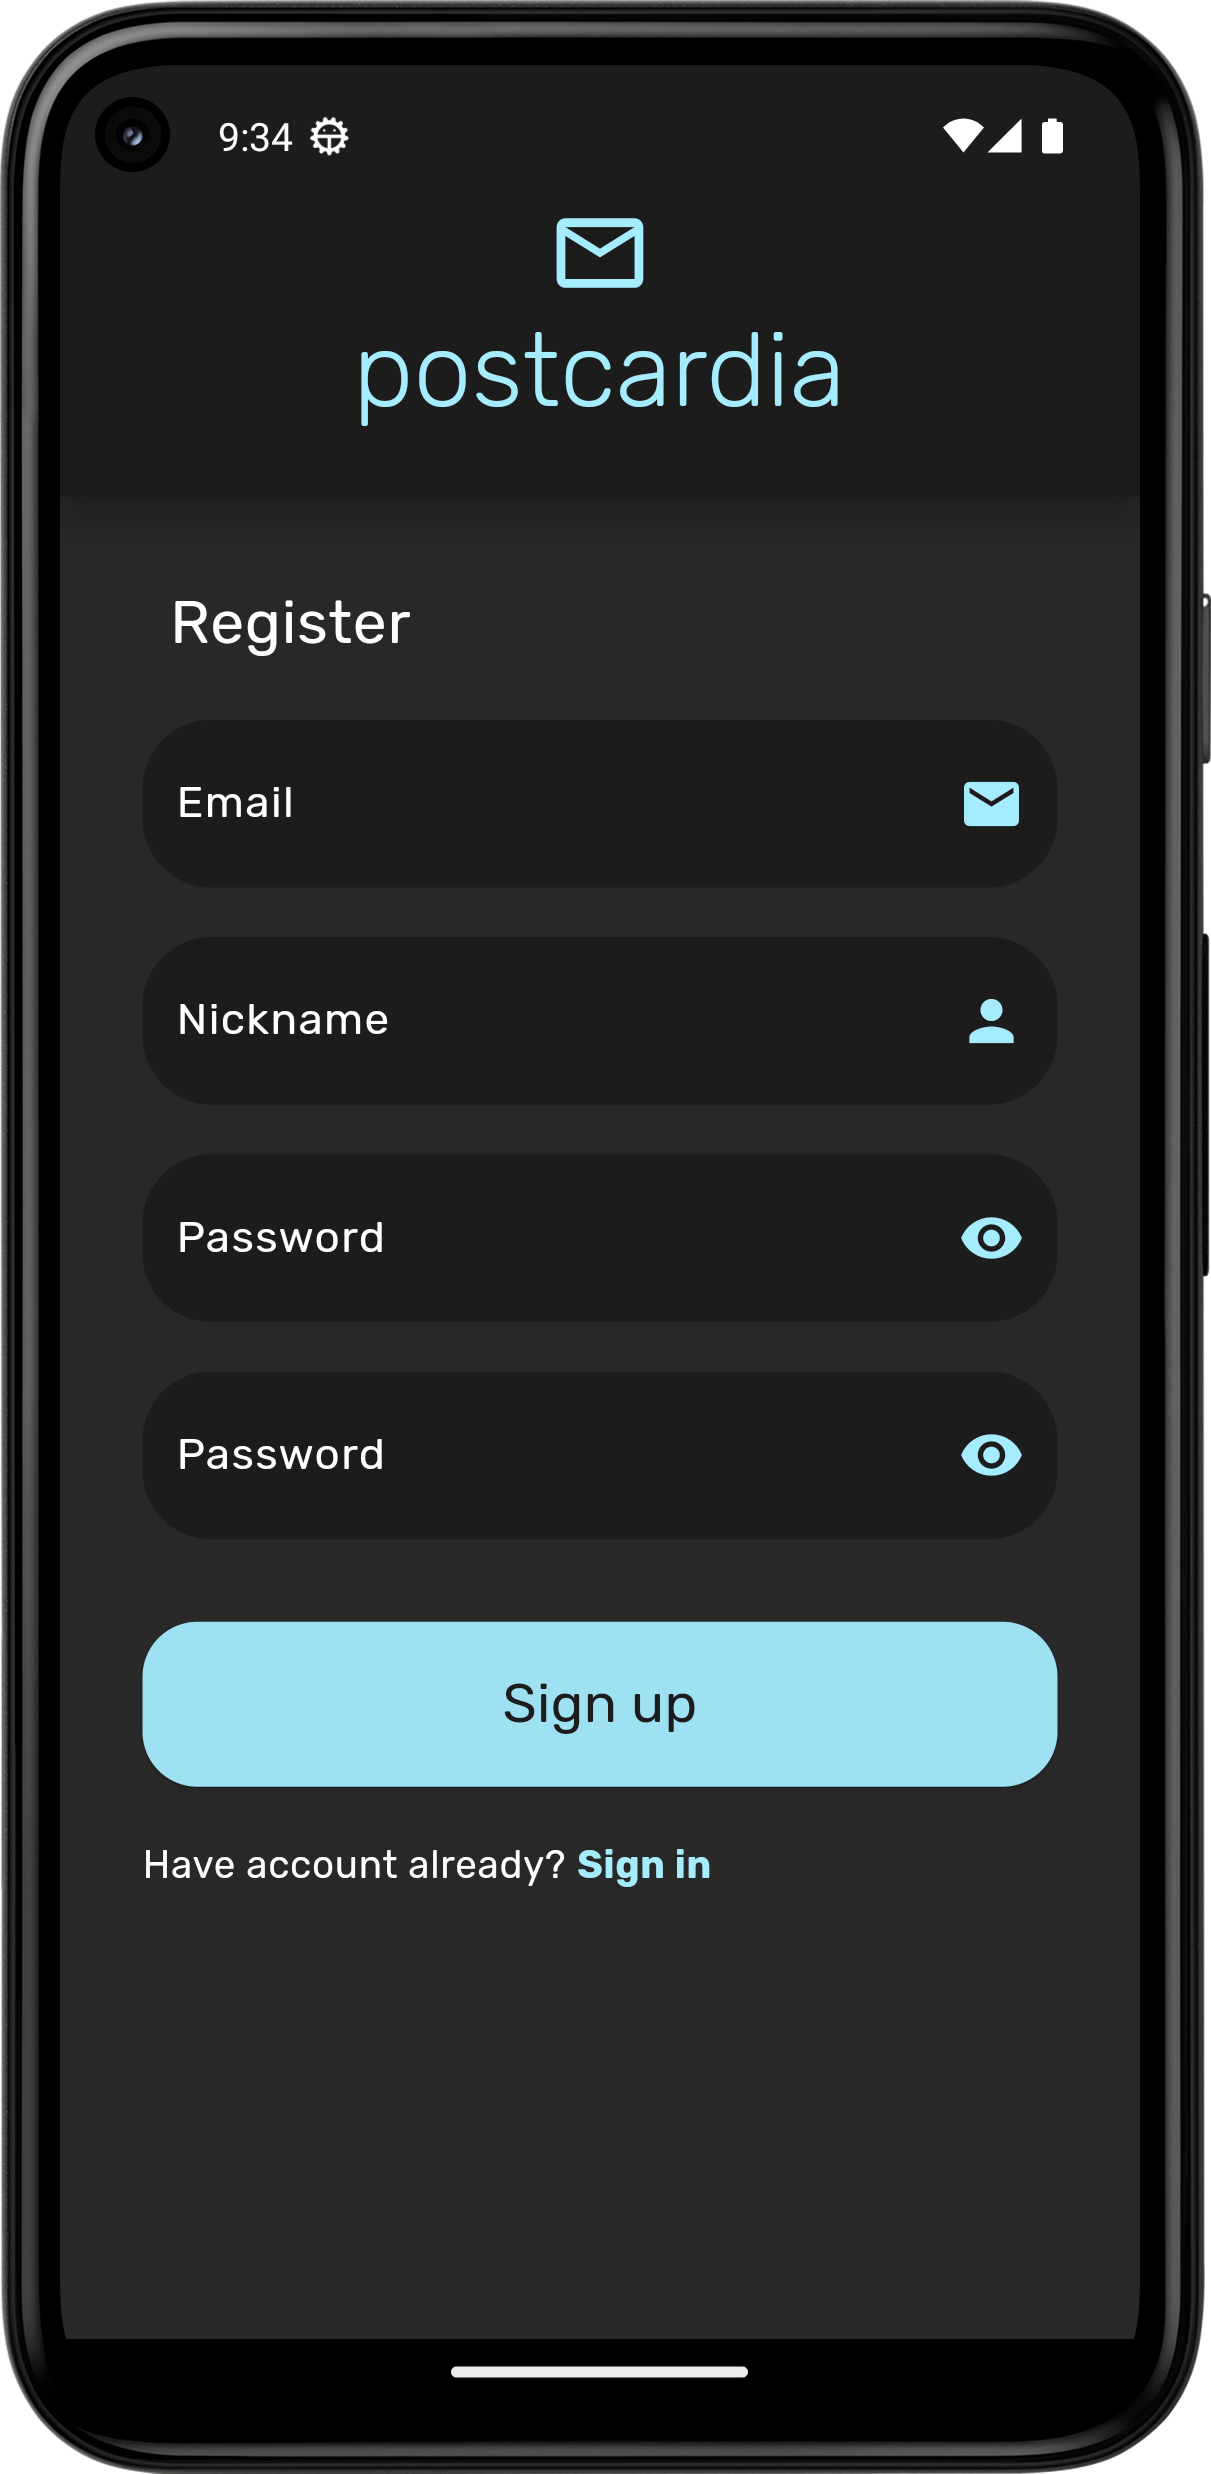
\includegraphics[width=0.5\textwidth]{mobile_ss/rejestracja.png}
    \caption{Strona do rejestracji użytkownika}
\end{figure}

Na stronie znajdują się cztery pola których wypełnienie jest wymagane. Symbol oka przy hasłach powoduje odsłonięcie hasła. Na dole strony znajduje się przycisk ``Sign in'', który przenosi użytkownika na stronę logowania. 
Po udanej rejestracji na dole ekranu pojawi się informacja na zielonym tle informująca o utworzeniu konta a użytkownik zostanie przekierowany na stronę logowania która wygląda jak na rysunku 5.9.

\begin{figure}[H]
    \centering
    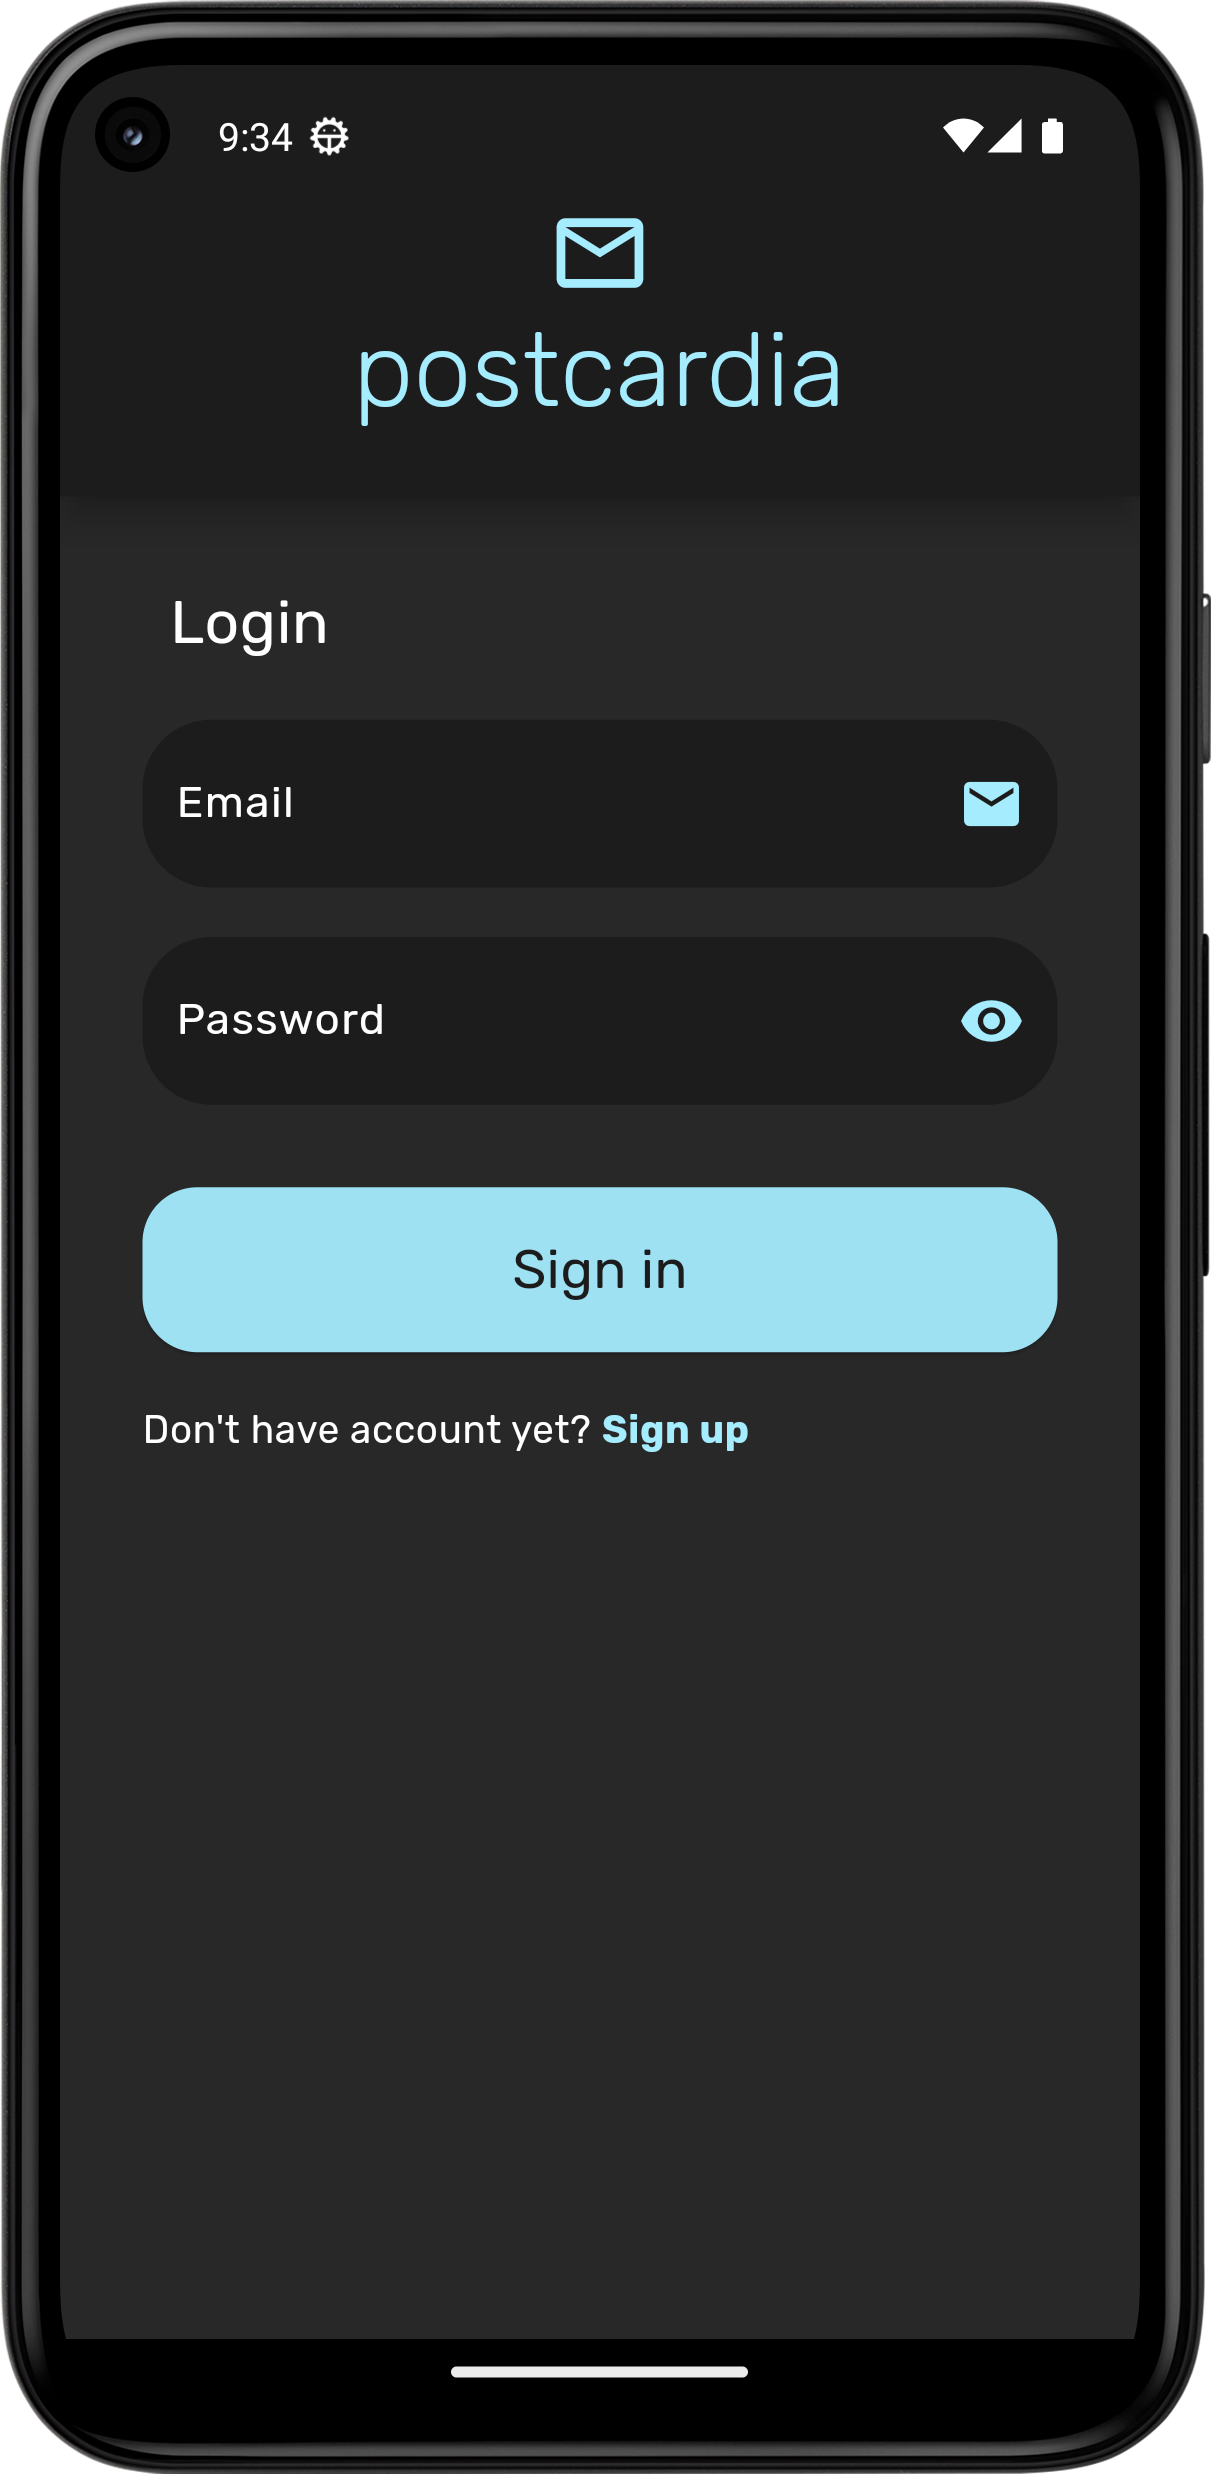
\includegraphics[width=0.5\textwidth]{mobile_ss/logowanie.png}
    \caption{Strona do logowania użytkownika}
\end{figure}

Na stronie logowania również posiadamy przycisk odsłaniający hasło a przycisk ``Sign up'' przenosi użytkownika do strony z rejestracją. 

\subsection{Nawigacja po aplikacji}
Nawigacja po aplikacji została wykonana w postaci szuflady. Każdy dział aplikacji posiada odpowiednią podstronę. Dodatkowo administrator posiada podstronę do zarządzania pocztówkami znajdującymi się w bazie danych oraz każdy typ użytkownika posiada przycisk wylogowujący na dole szuflady.

\begin{figure}[H]
    \centering
    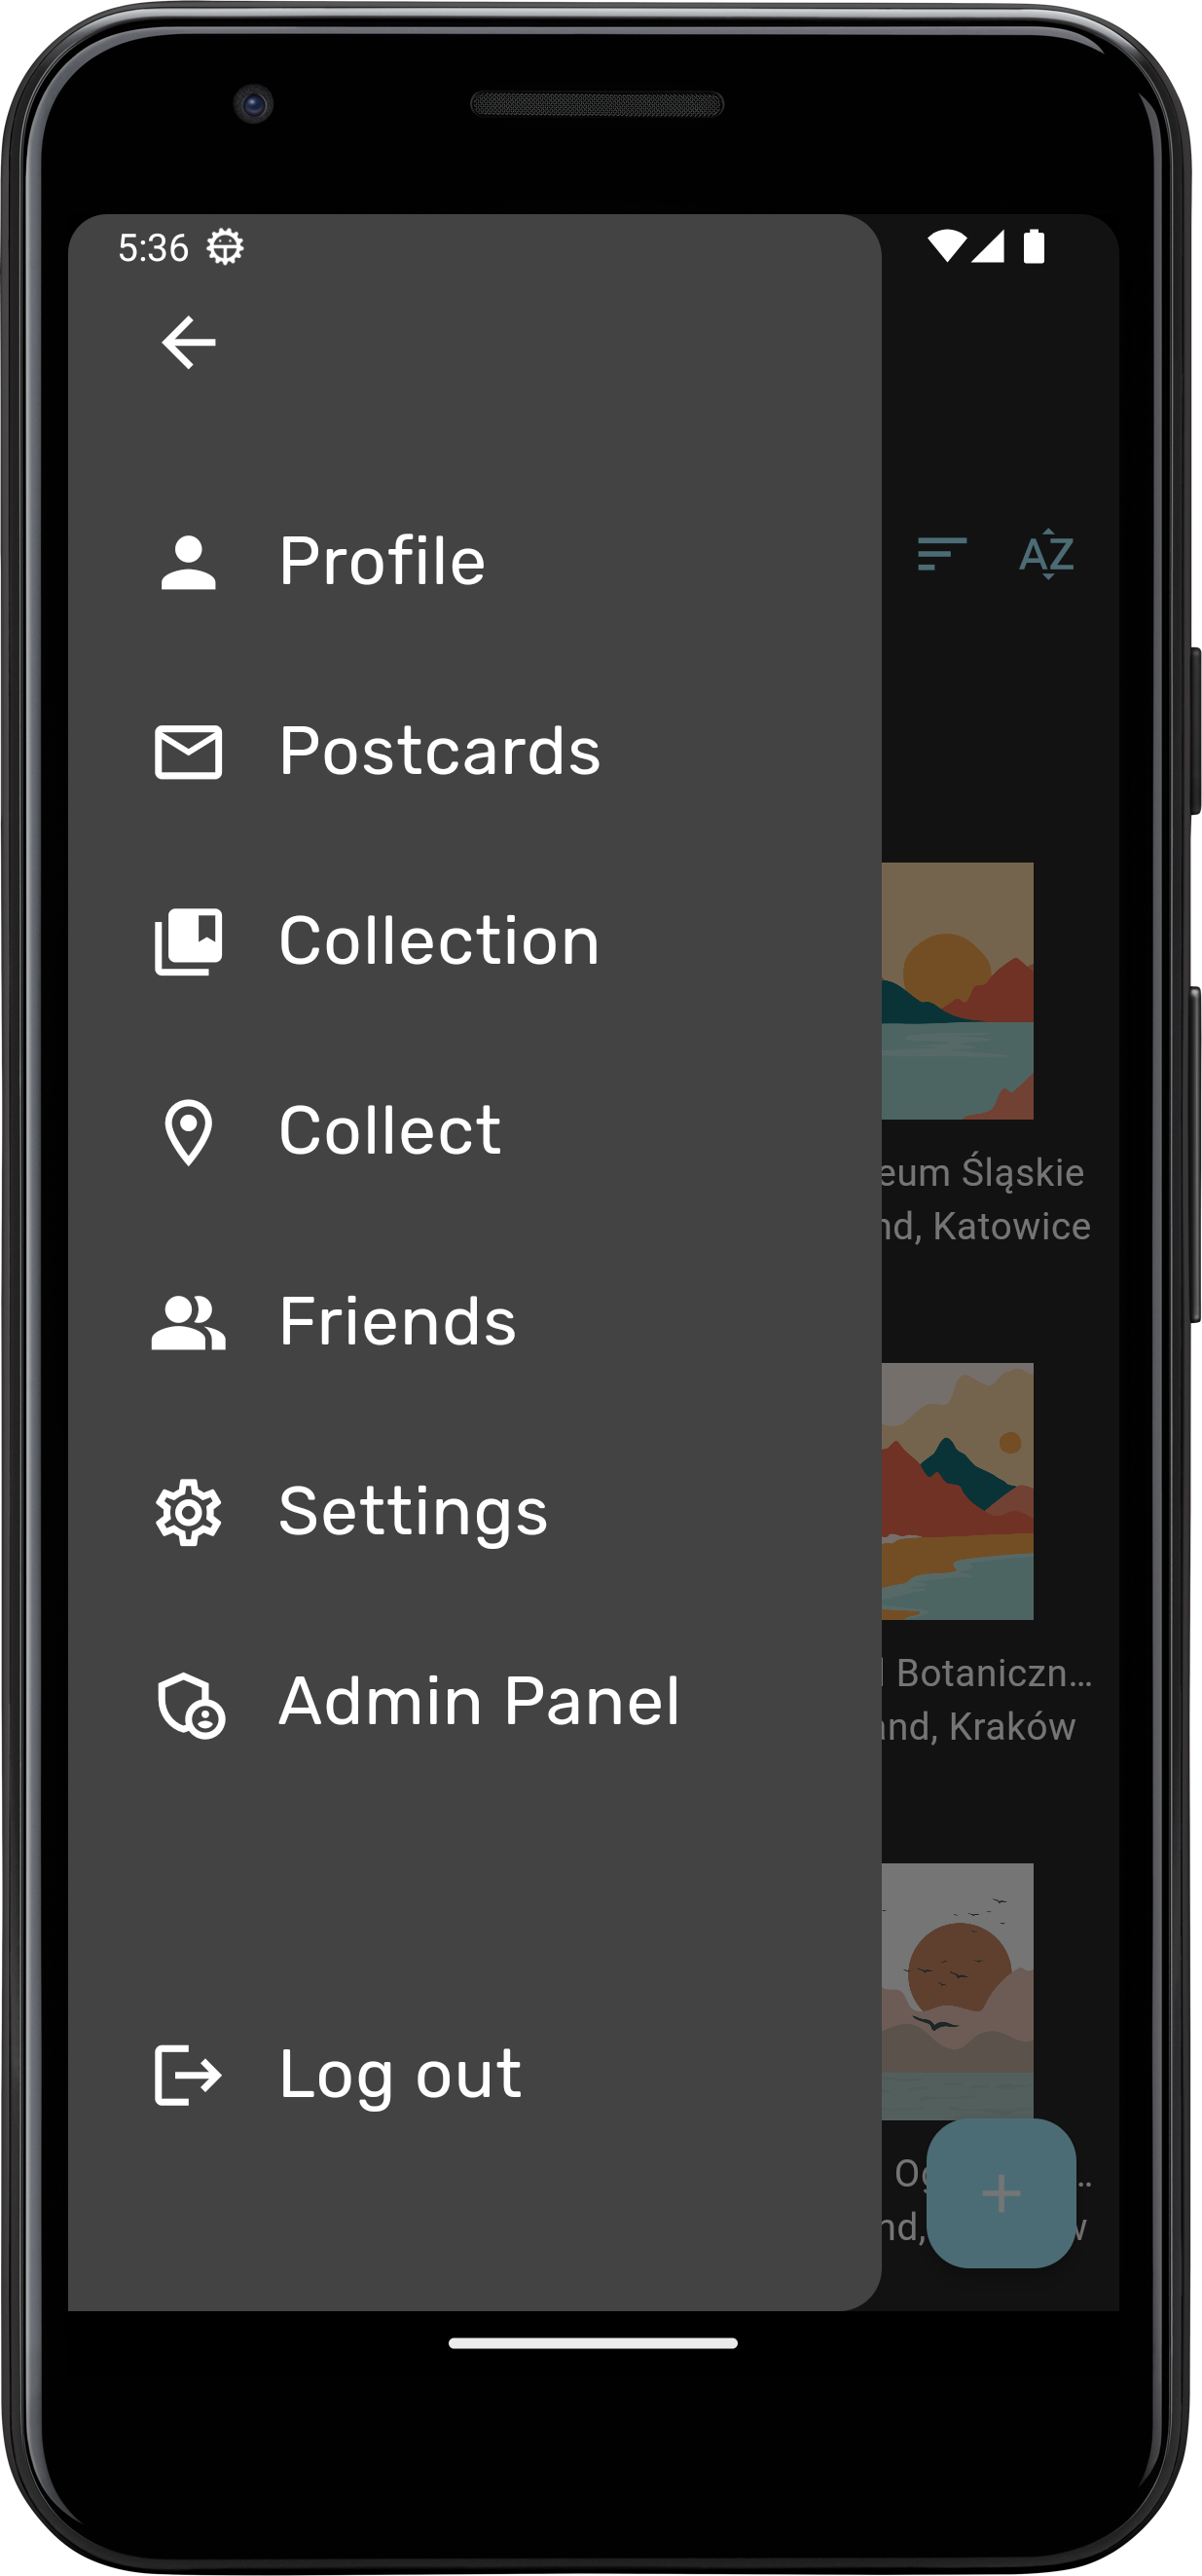
\includegraphics[width=0.5\textwidth]{mobile_ss/szuflada.png}
    \caption{Szuflada służąca do nawigacji}
\end{figure}

\subsection{Edycja konta i informacji}
W aplikacji możemy zobaczyć jak inni widzą nasz profil wchodząc na stronę ``Profile page'', która została przedstawiona na rysunku 5.11.

\begin{figure}[H]
    \centering
    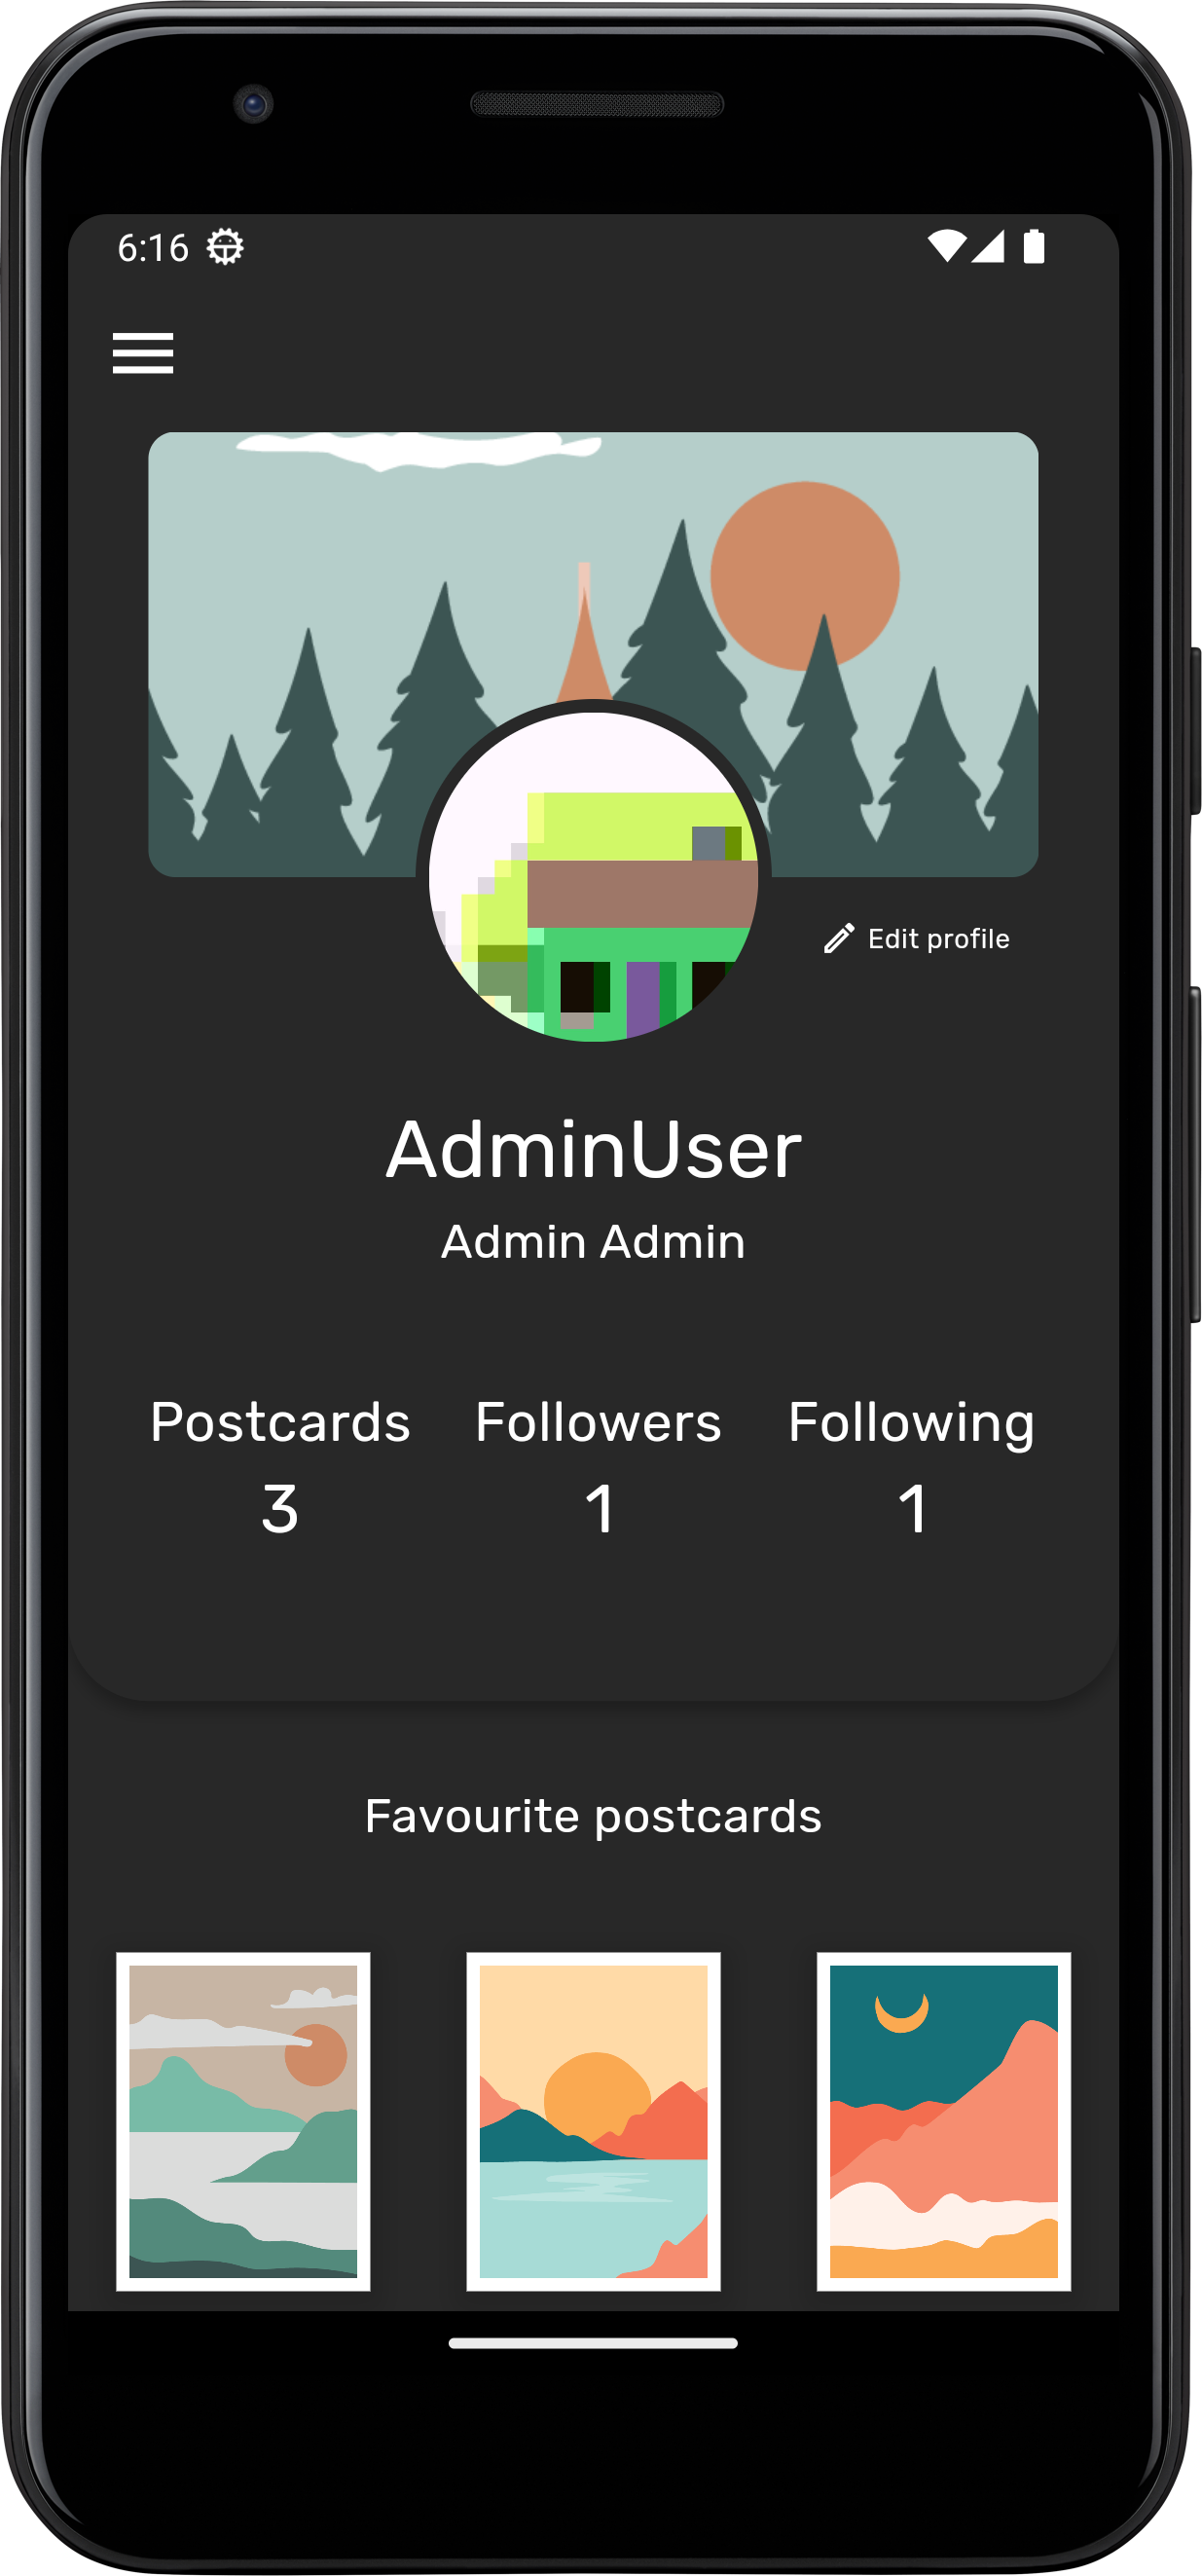
\includegraphics[width=0.5\textwidth]{mobile_ss/profil_bez_info.png}
    \caption{Strona z profilem użytkownika bez informacji}
\end{figure}

Na powyższym zrzucie ekranu widzimy profil, który posiada dwie ulubione pocztówki ale nie ma jeszcze wprowadzonych danych oraz zdjęć. Aby takowe wprowadzić należy przejść do strony edycji profilu używając przycisku ``Edit profile'' znajdującego się po prawej stronie. Użytkownik zostanie wtedy przeniesiony do strony edycji gdzie może wprowadzić swoje dane osobowe. Każda z rubryk jest nieobowiązkowa. Użytkownik sam może wybrać jakie dane chce, aby się wyświetlały na jego profilu. Na rysunkach 5.12 i 5.13 znajdują się zrzuty ekranu obrazujące proces wprowadzania informacji do profilu.

\begin{figure}[H]
  \centering
  \begin{minipage}[b]{0.49\textwidth}
    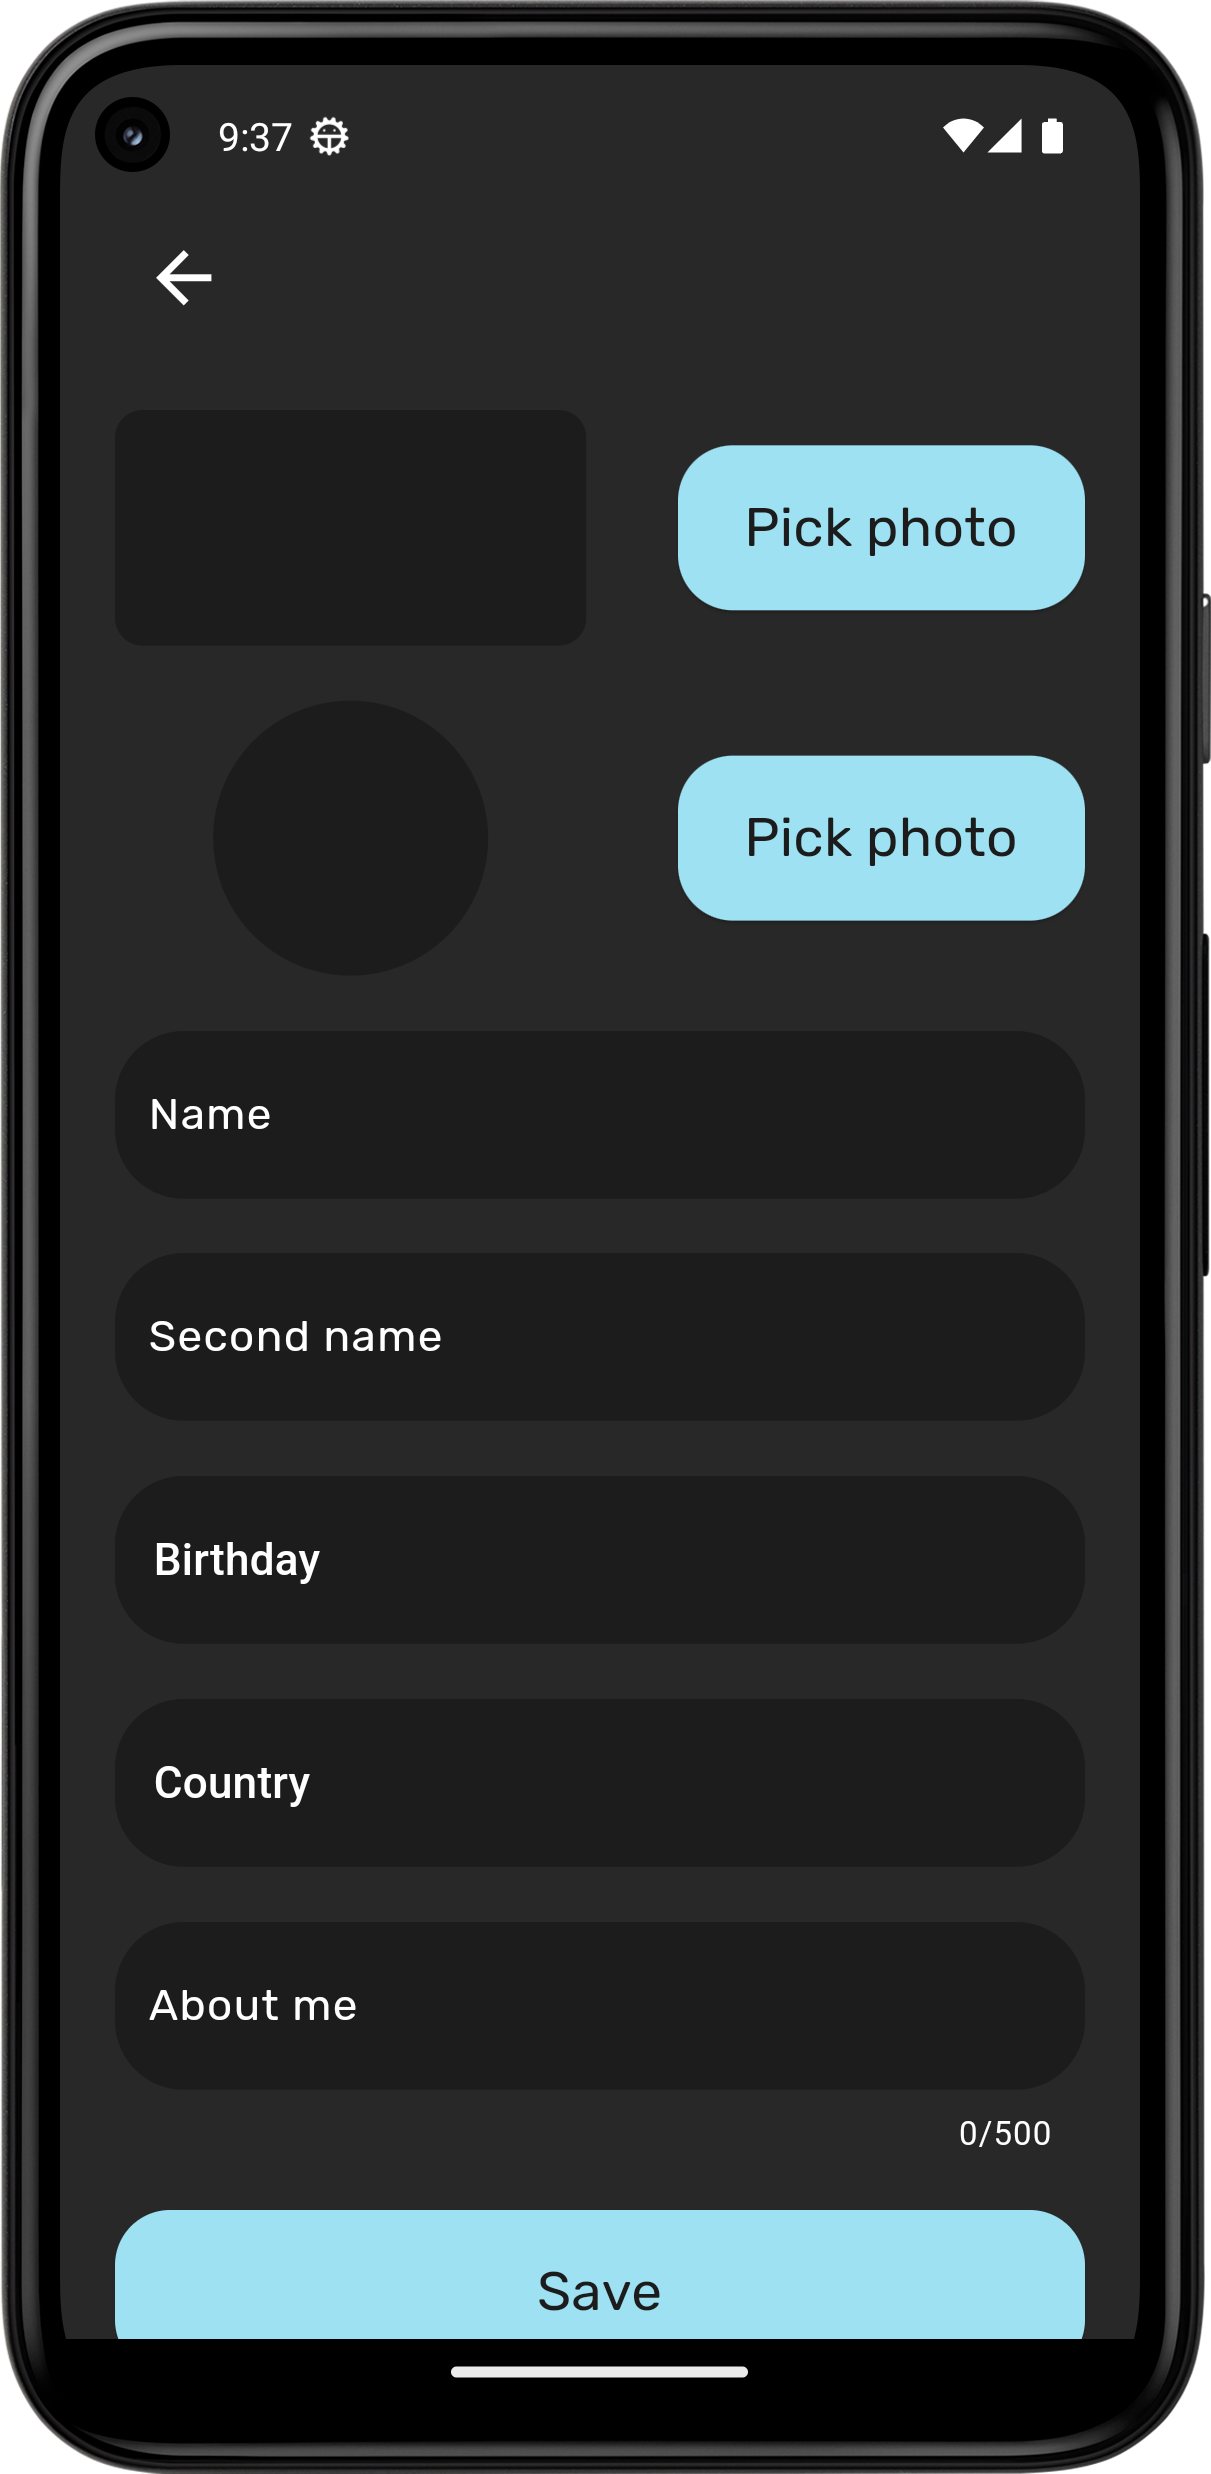
\includegraphics[width=\textwidth]{mobile_ss/edycja_profilu_bez_danych.png}
    \caption{Edycja profilu bez wprowadzonych danych}
  \end{minipage}
  \hfill
  \begin{minipage}[b]{0.49\textwidth}
    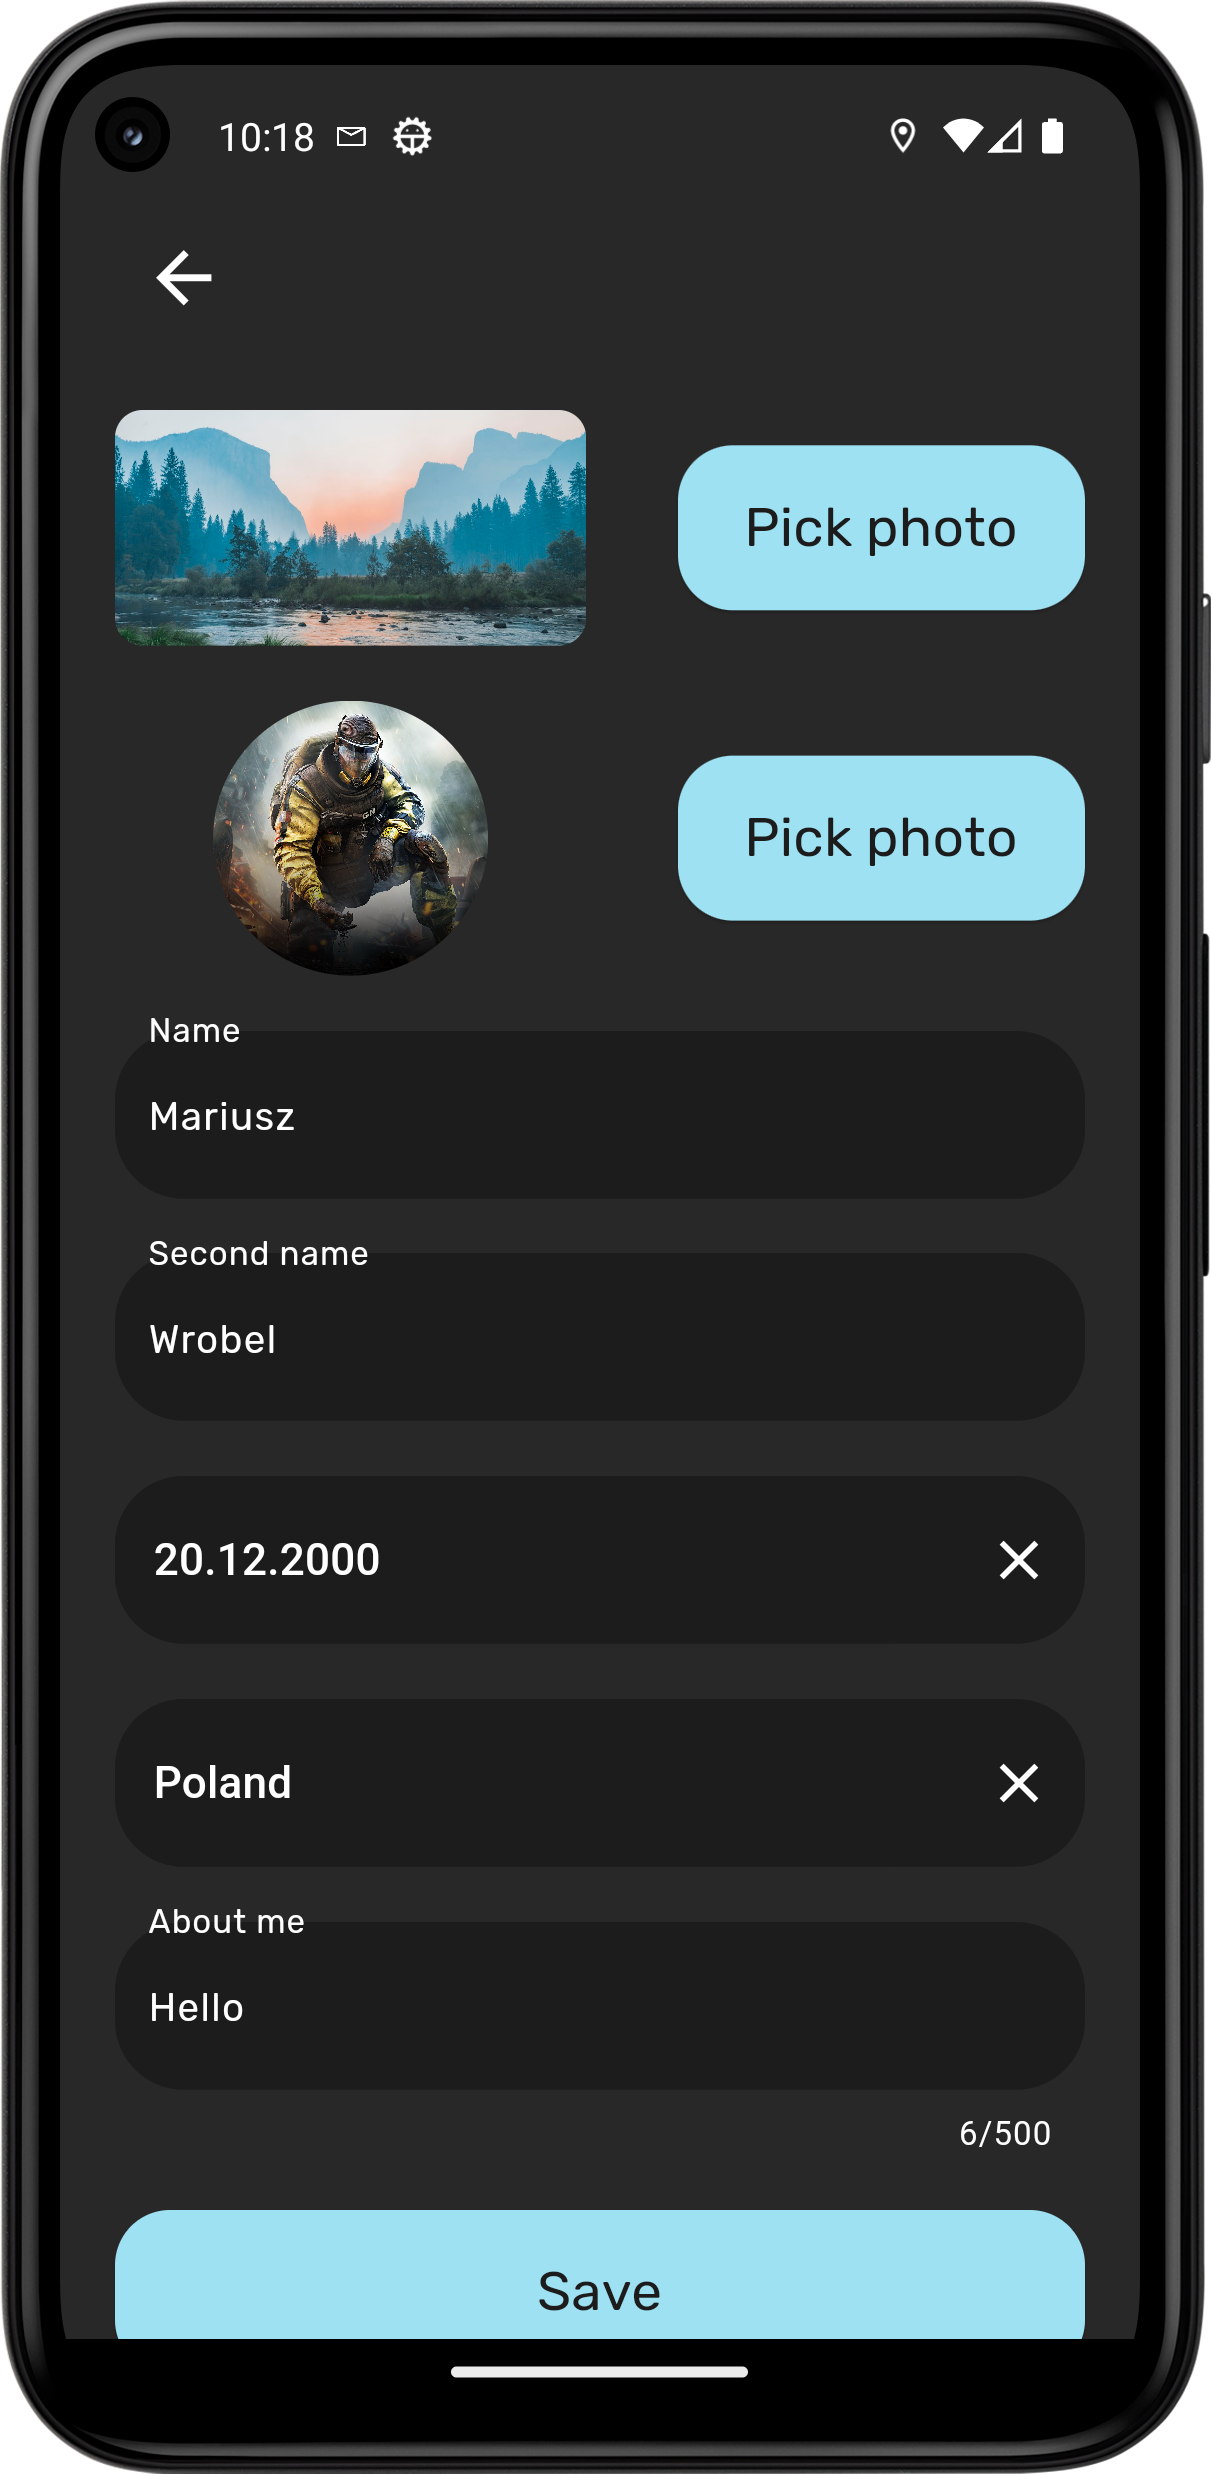
\includegraphics[width=\textwidth]{mobile_ss/edycja_profilu_z_danymi.png}
    \caption{Edycja profilu z wprowadzonymi danymi}
  \end{minipage}
\end{figure}

Po wprowadzeniu danych nasz profil prezentuje się jak na rysunku 5.14.

\begin{figure}[H]
    \centering
    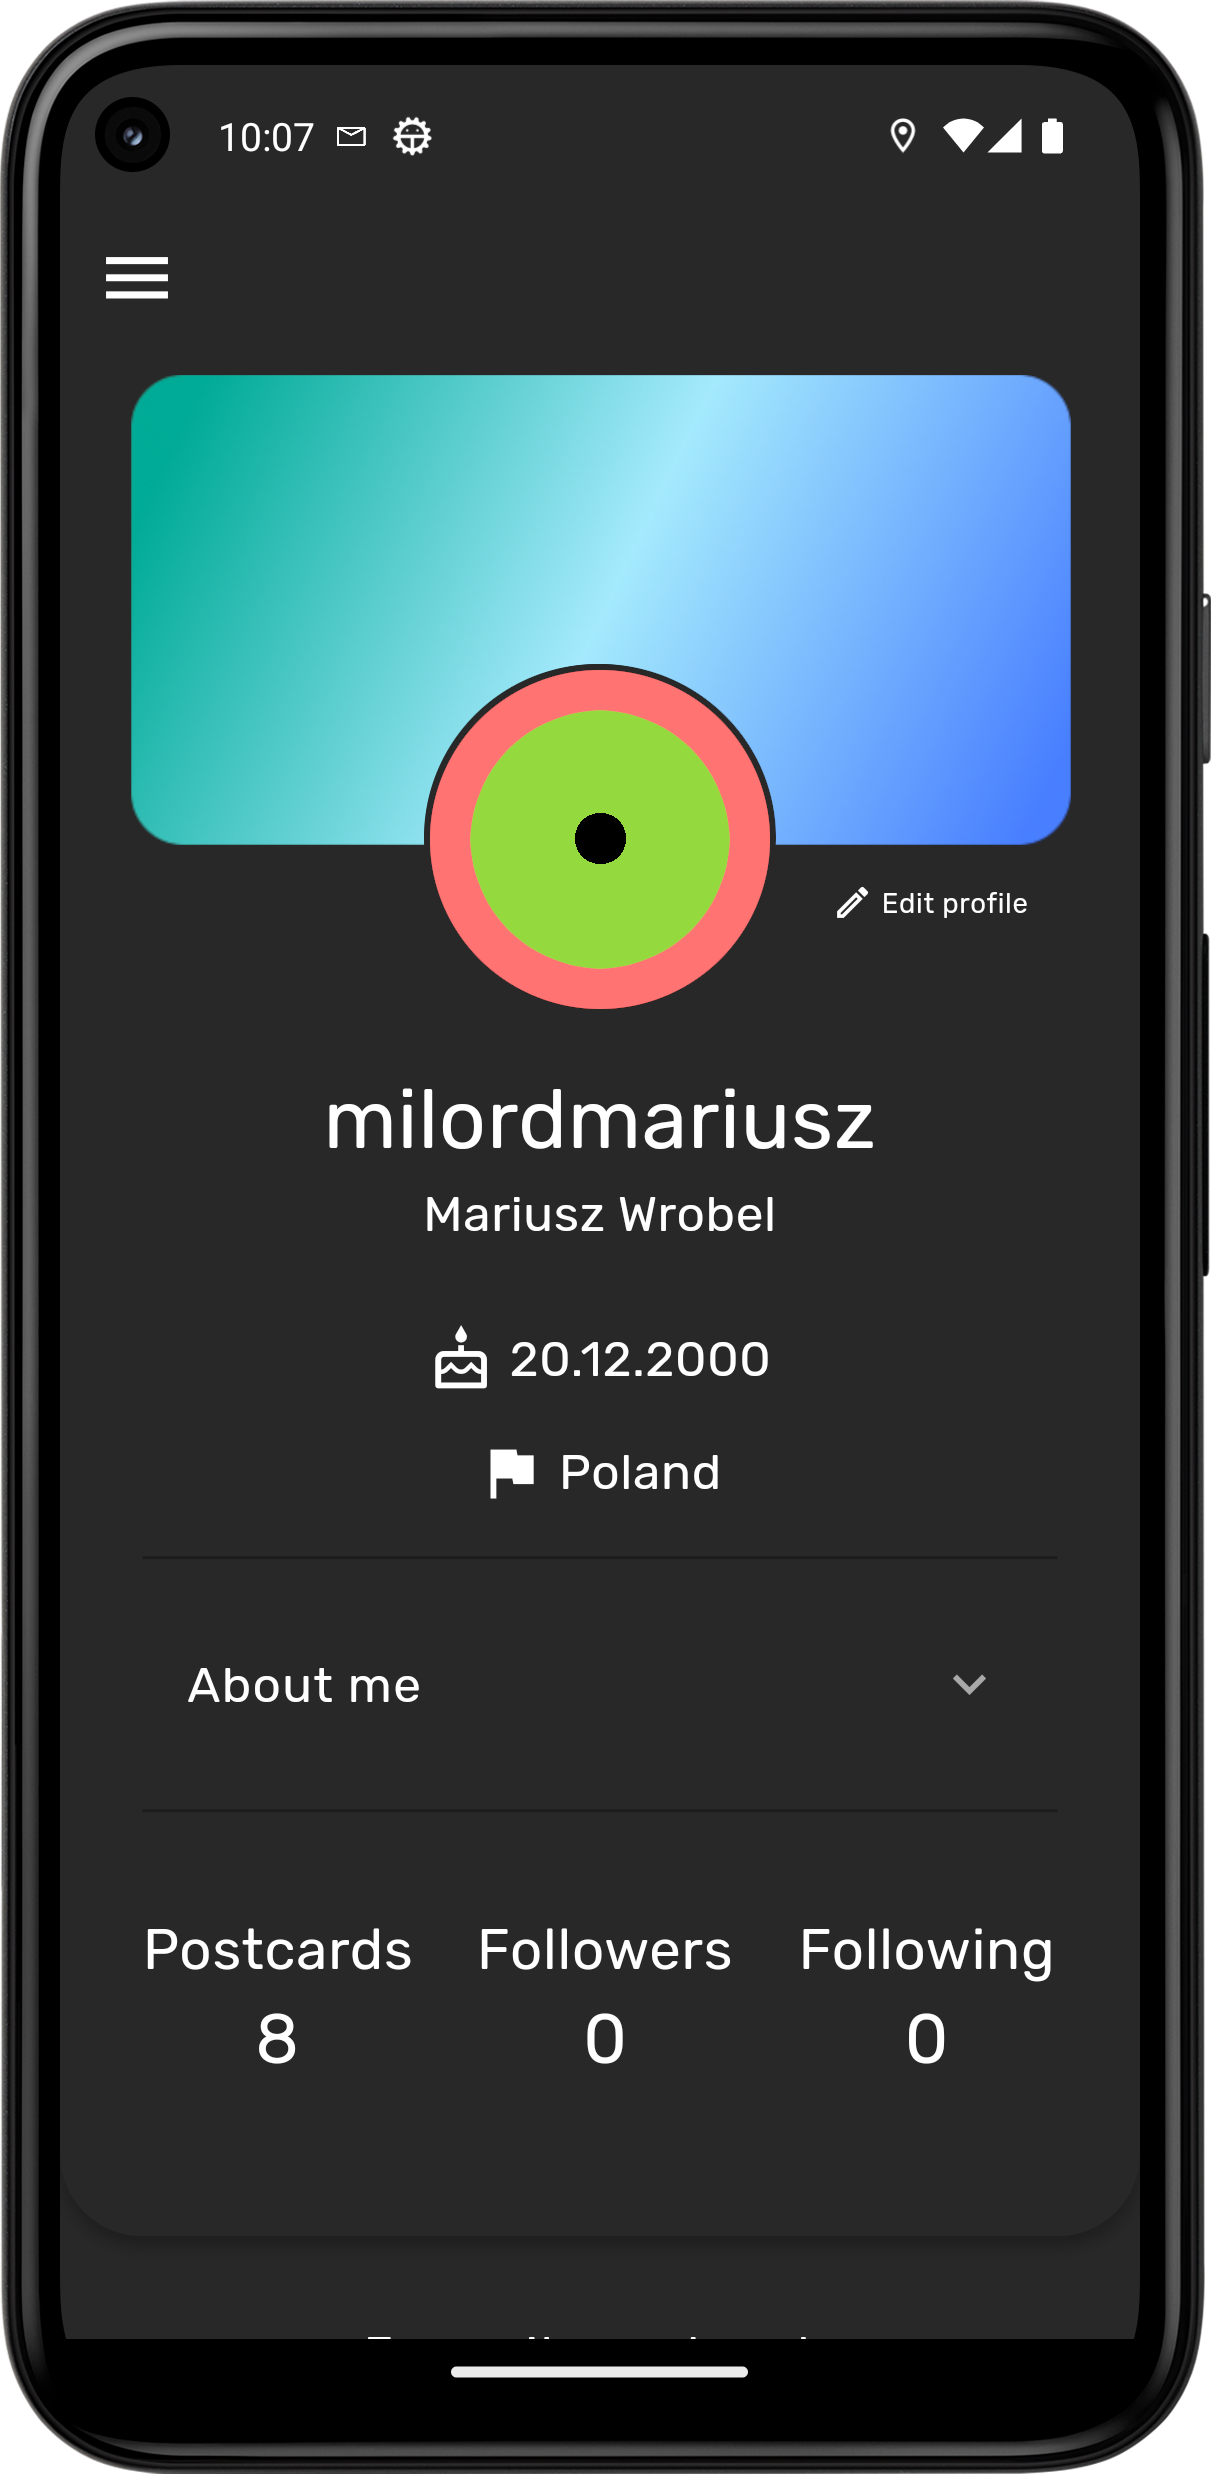
\includegraphics[width=0.5\textwidth]{mobile_ss/profil_z_info.png}
    \caption{Strona z profilem użytkownika bez informacji}
\end{figure}

\subsection{Kolekcja}
Kolekcja to dział w którym możemy zobaczyć wszystkie pocztówki, które kiedykolwiek odebraliśmy nawet jeżeli pocztówkę z tego miejsca komuś wysłaliśmy. Pierwsza zakładka to nasza kolekcja, która wygląda następująco. 

\begin{figure}[H]
    \centering
    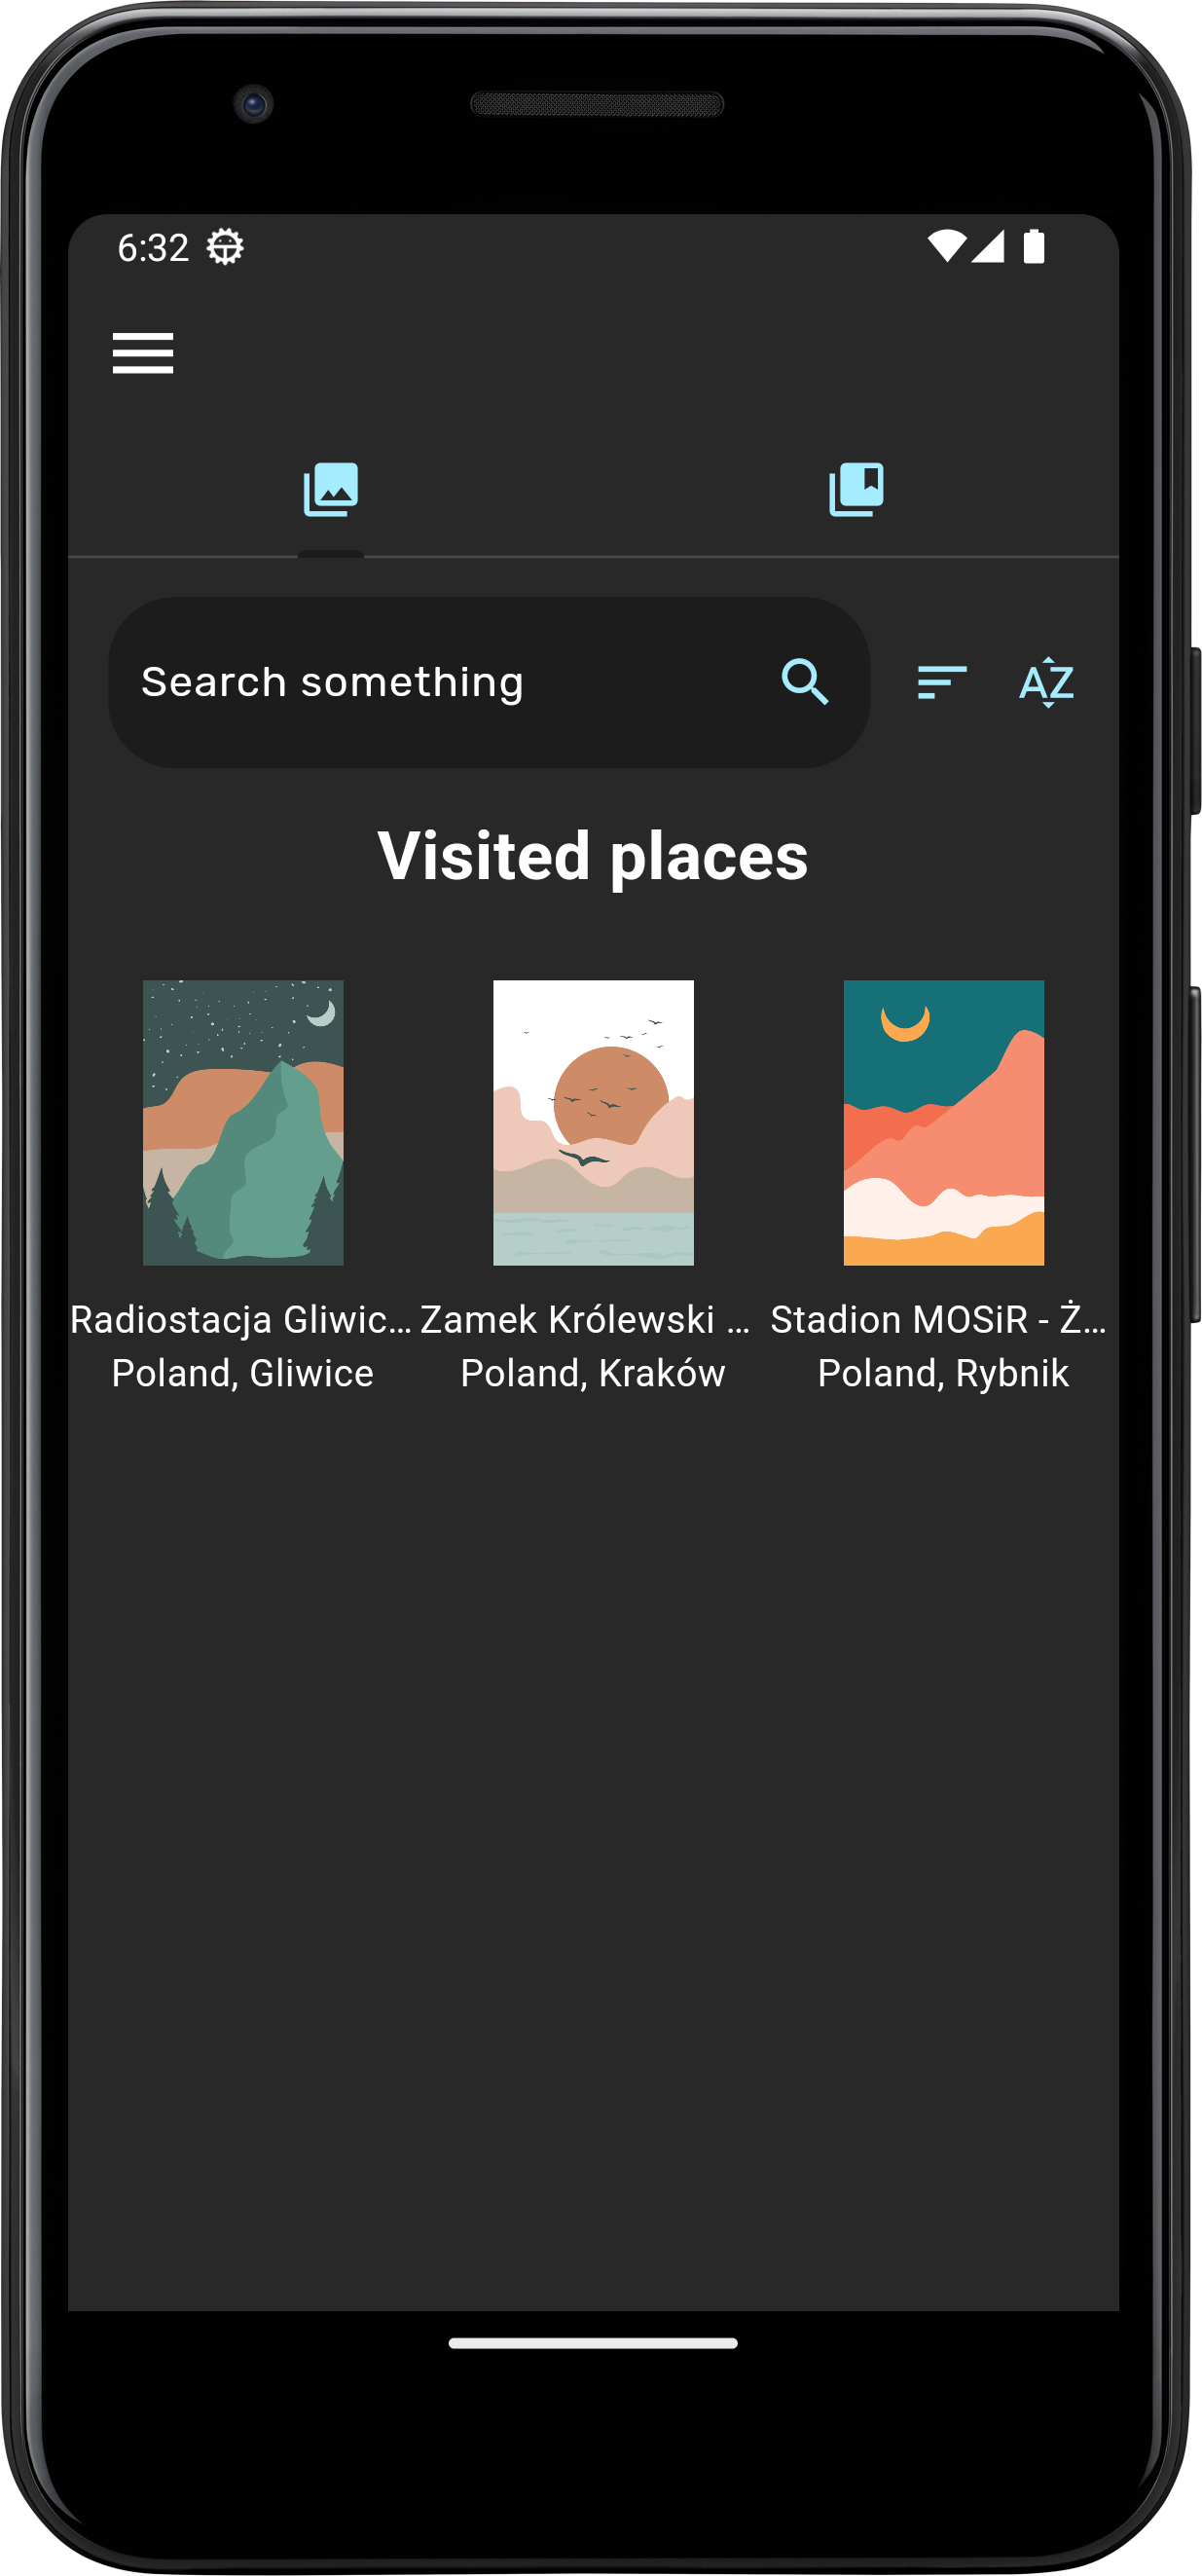
\includegraphics[width=0.5\textwidth]{mobile_ss/obrazki_nasze.png}
    \caption{Widok zakładki z naszą kolekcją}
\end{figure}

Druga zakładka to wszystkie pocztówki, które można zebrać. Jeżeli dana pocztówka znajduje się w naszej kolekcji to jest ona kolorowa, jeżeli danej pocztówki jeszcze nie uzyskaliśmy, będzie ona czarno biała. 

\begin{figure}[H]
    \centering
    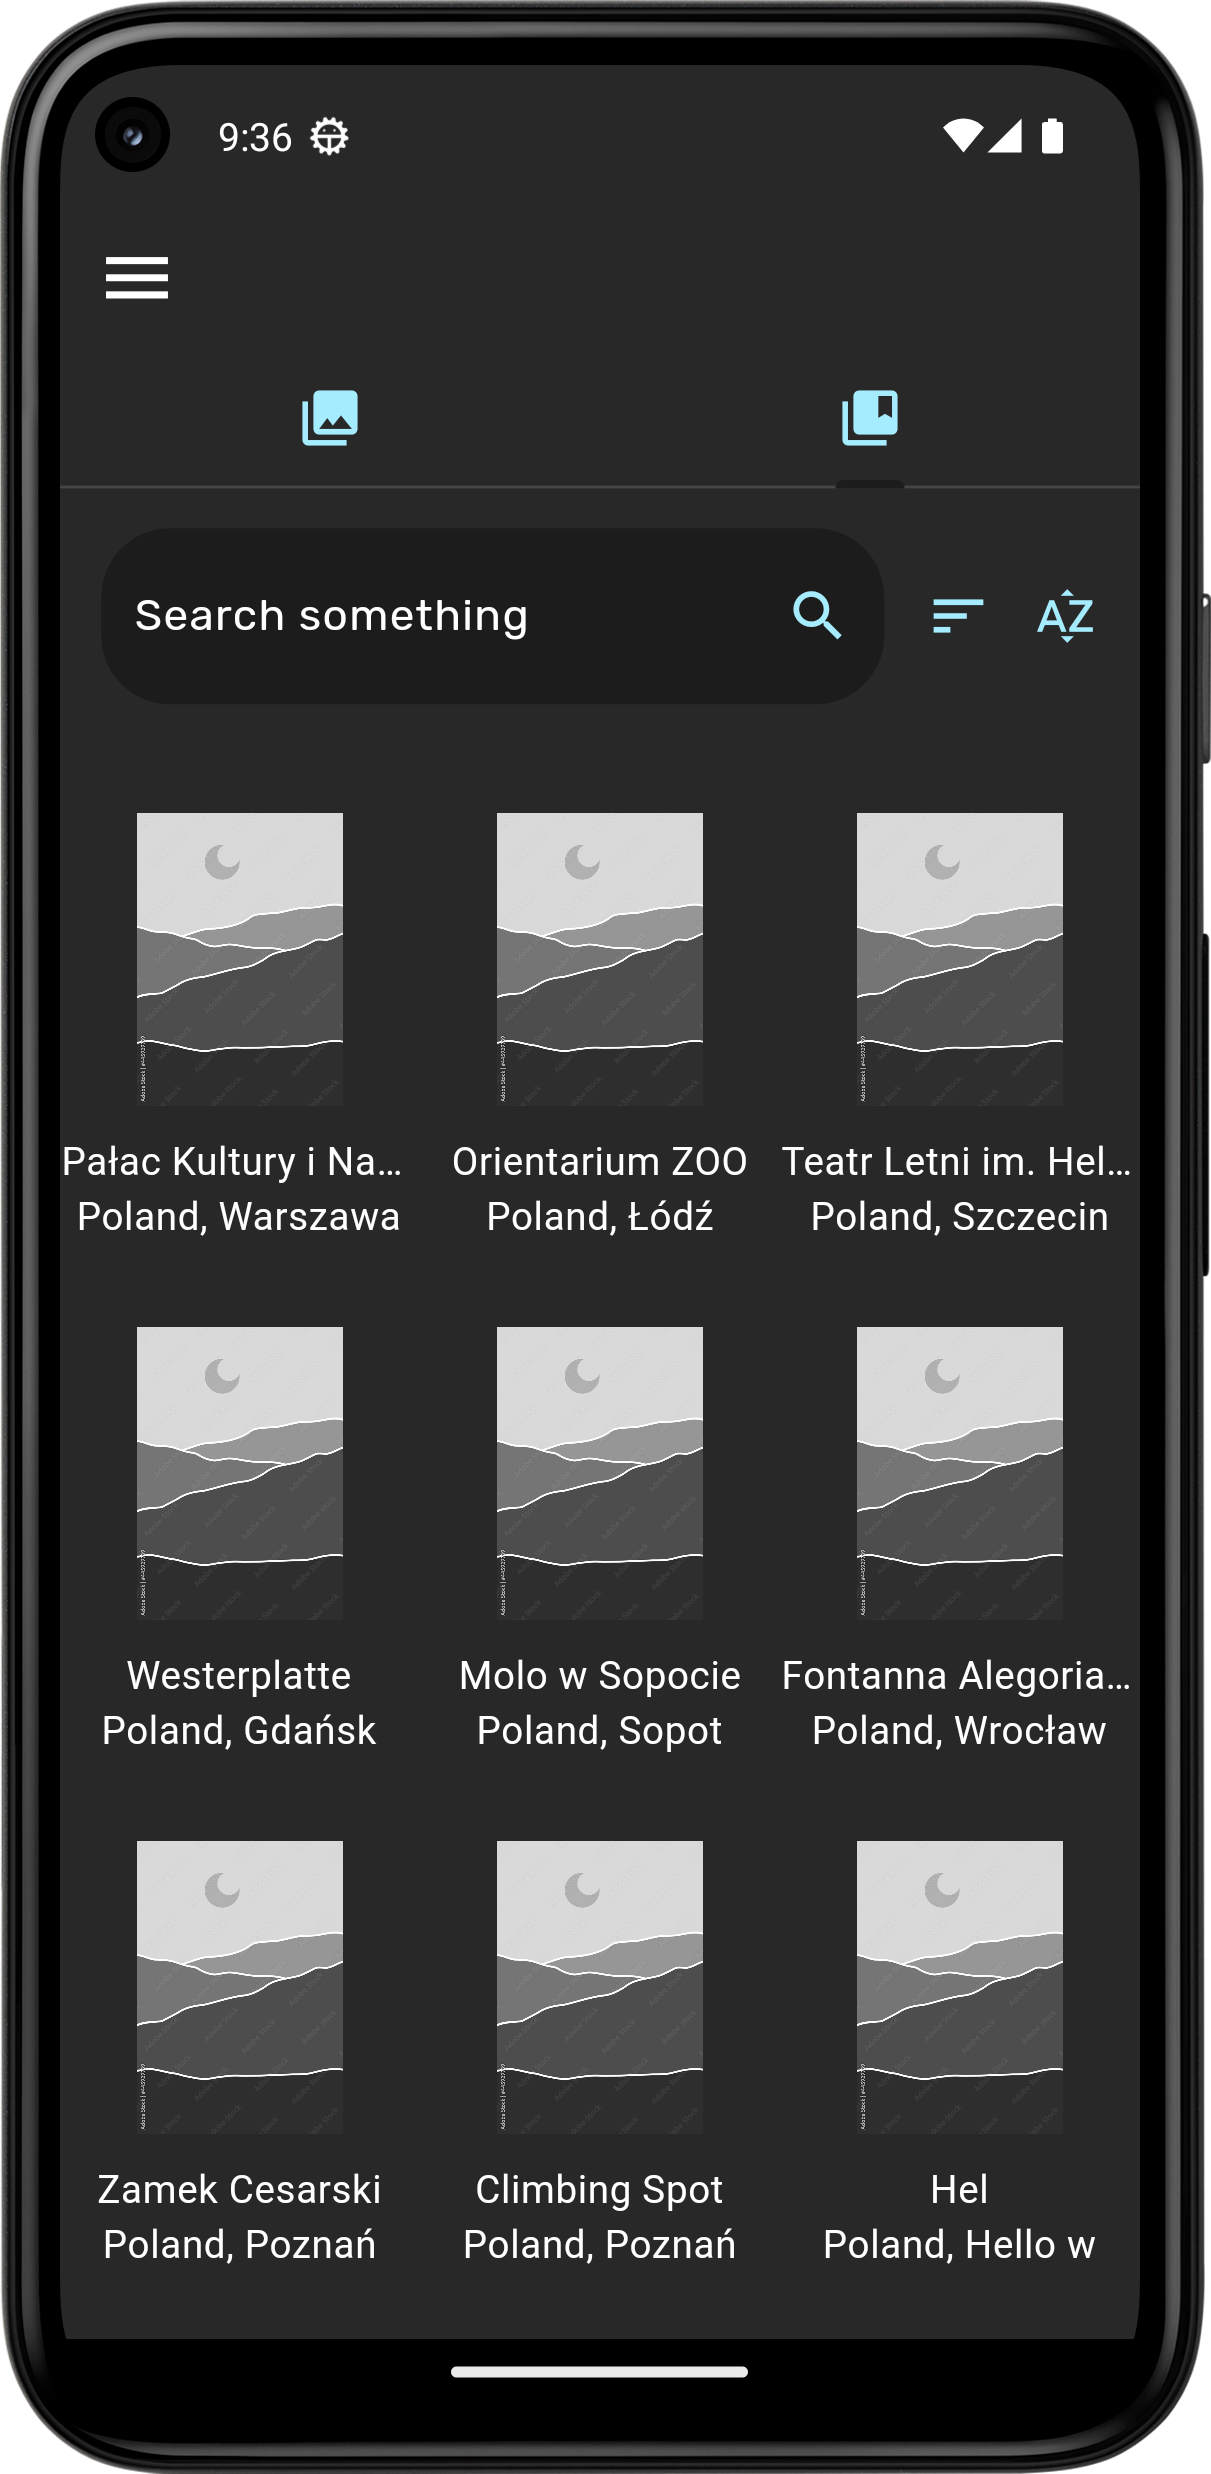
\includegraphics[width=0.5\textwidth]{mobile_ss/obrazki_wszystkie.png}
    \caption{Widok zakładki z naszą kolekcją}
\end{figure}

Na obu zakładkach możemy wyszukiwać daną pocztówkę po nazwie, filtrować pocztówki oraz je sortować. 

\subsection{Pocztówki}
Pocztówki to podstrona, która zawiera te pocztówki, które zebraliśmy i możemy wysłać jak i również te, które otrzymaliśmy od innych użytkowników. W pierwszej zakładce znajdują się pocztówki, które możemy komuś wysłać. Możemy te pocztówki tak samo jak w przypadku kolekcji filtrować, wyszukiwać i sortować. Po wciśnięciu danej pocztówki pojawia się dodatkowe okienko ukazujące więcej szczegółów dotyczące danej pocztówki. 

\begin{figure}[H]
  \centering
  \begin{minipage}[b]{0.49\textwidth}
    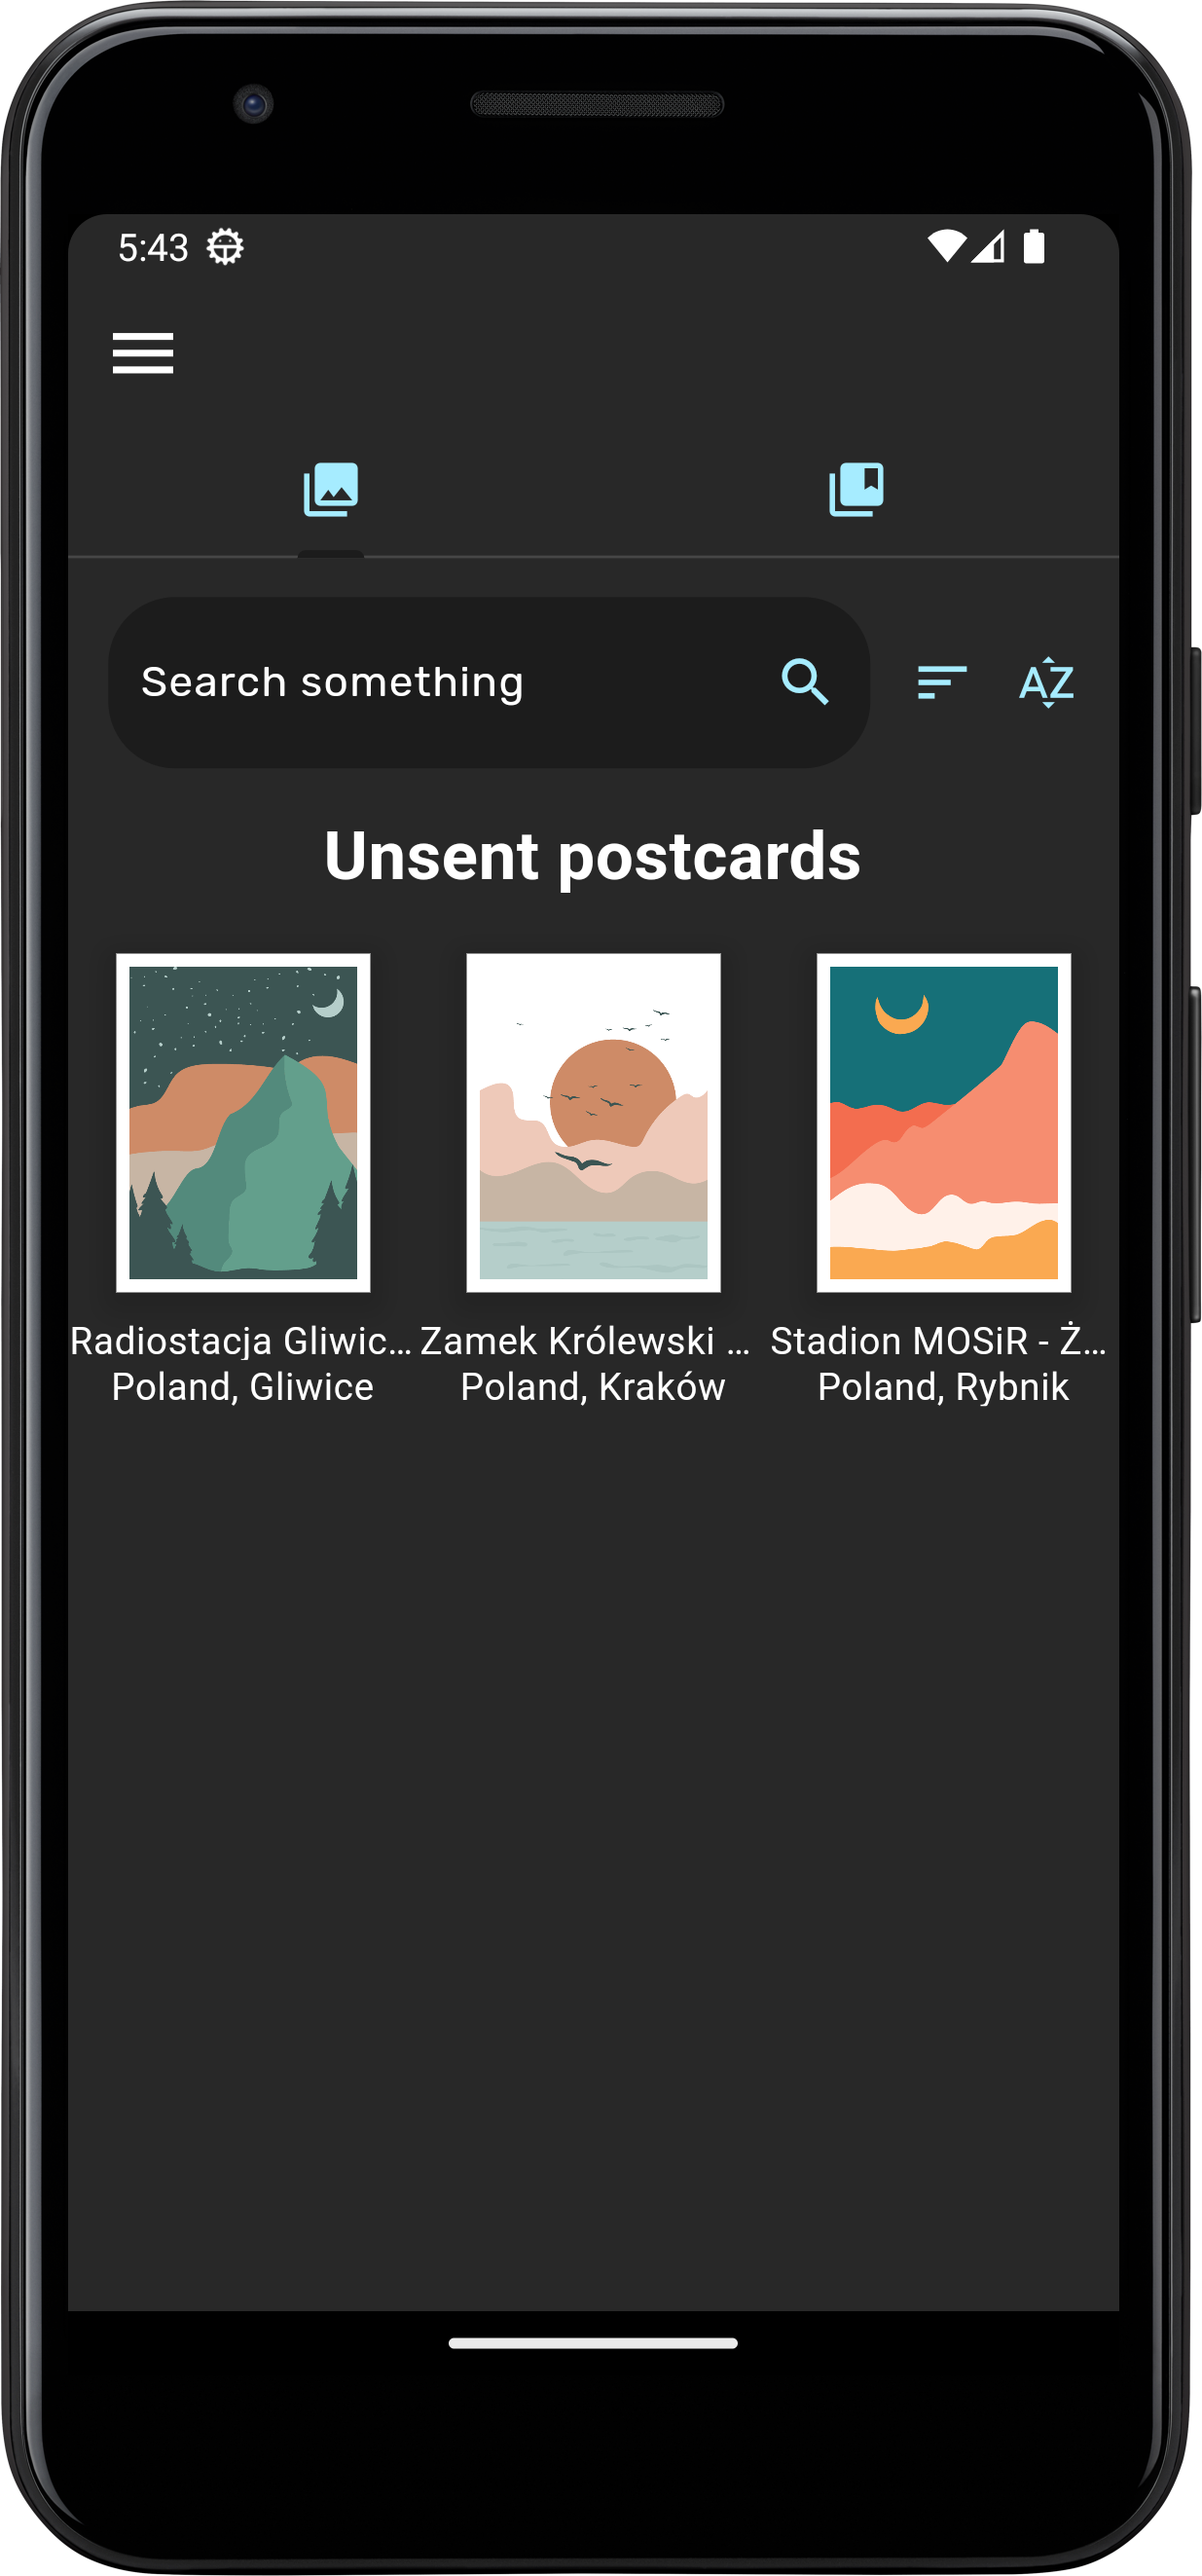
\includegraphics[width=\textwidth]{mobile_ss/pocztowki.png}
    \caption{Zawartość zakładki z pocztówkami do wysłania}
  \end{minipage}
  \hfill
  \begin{minipage}[b]{0.49\textwidth}
    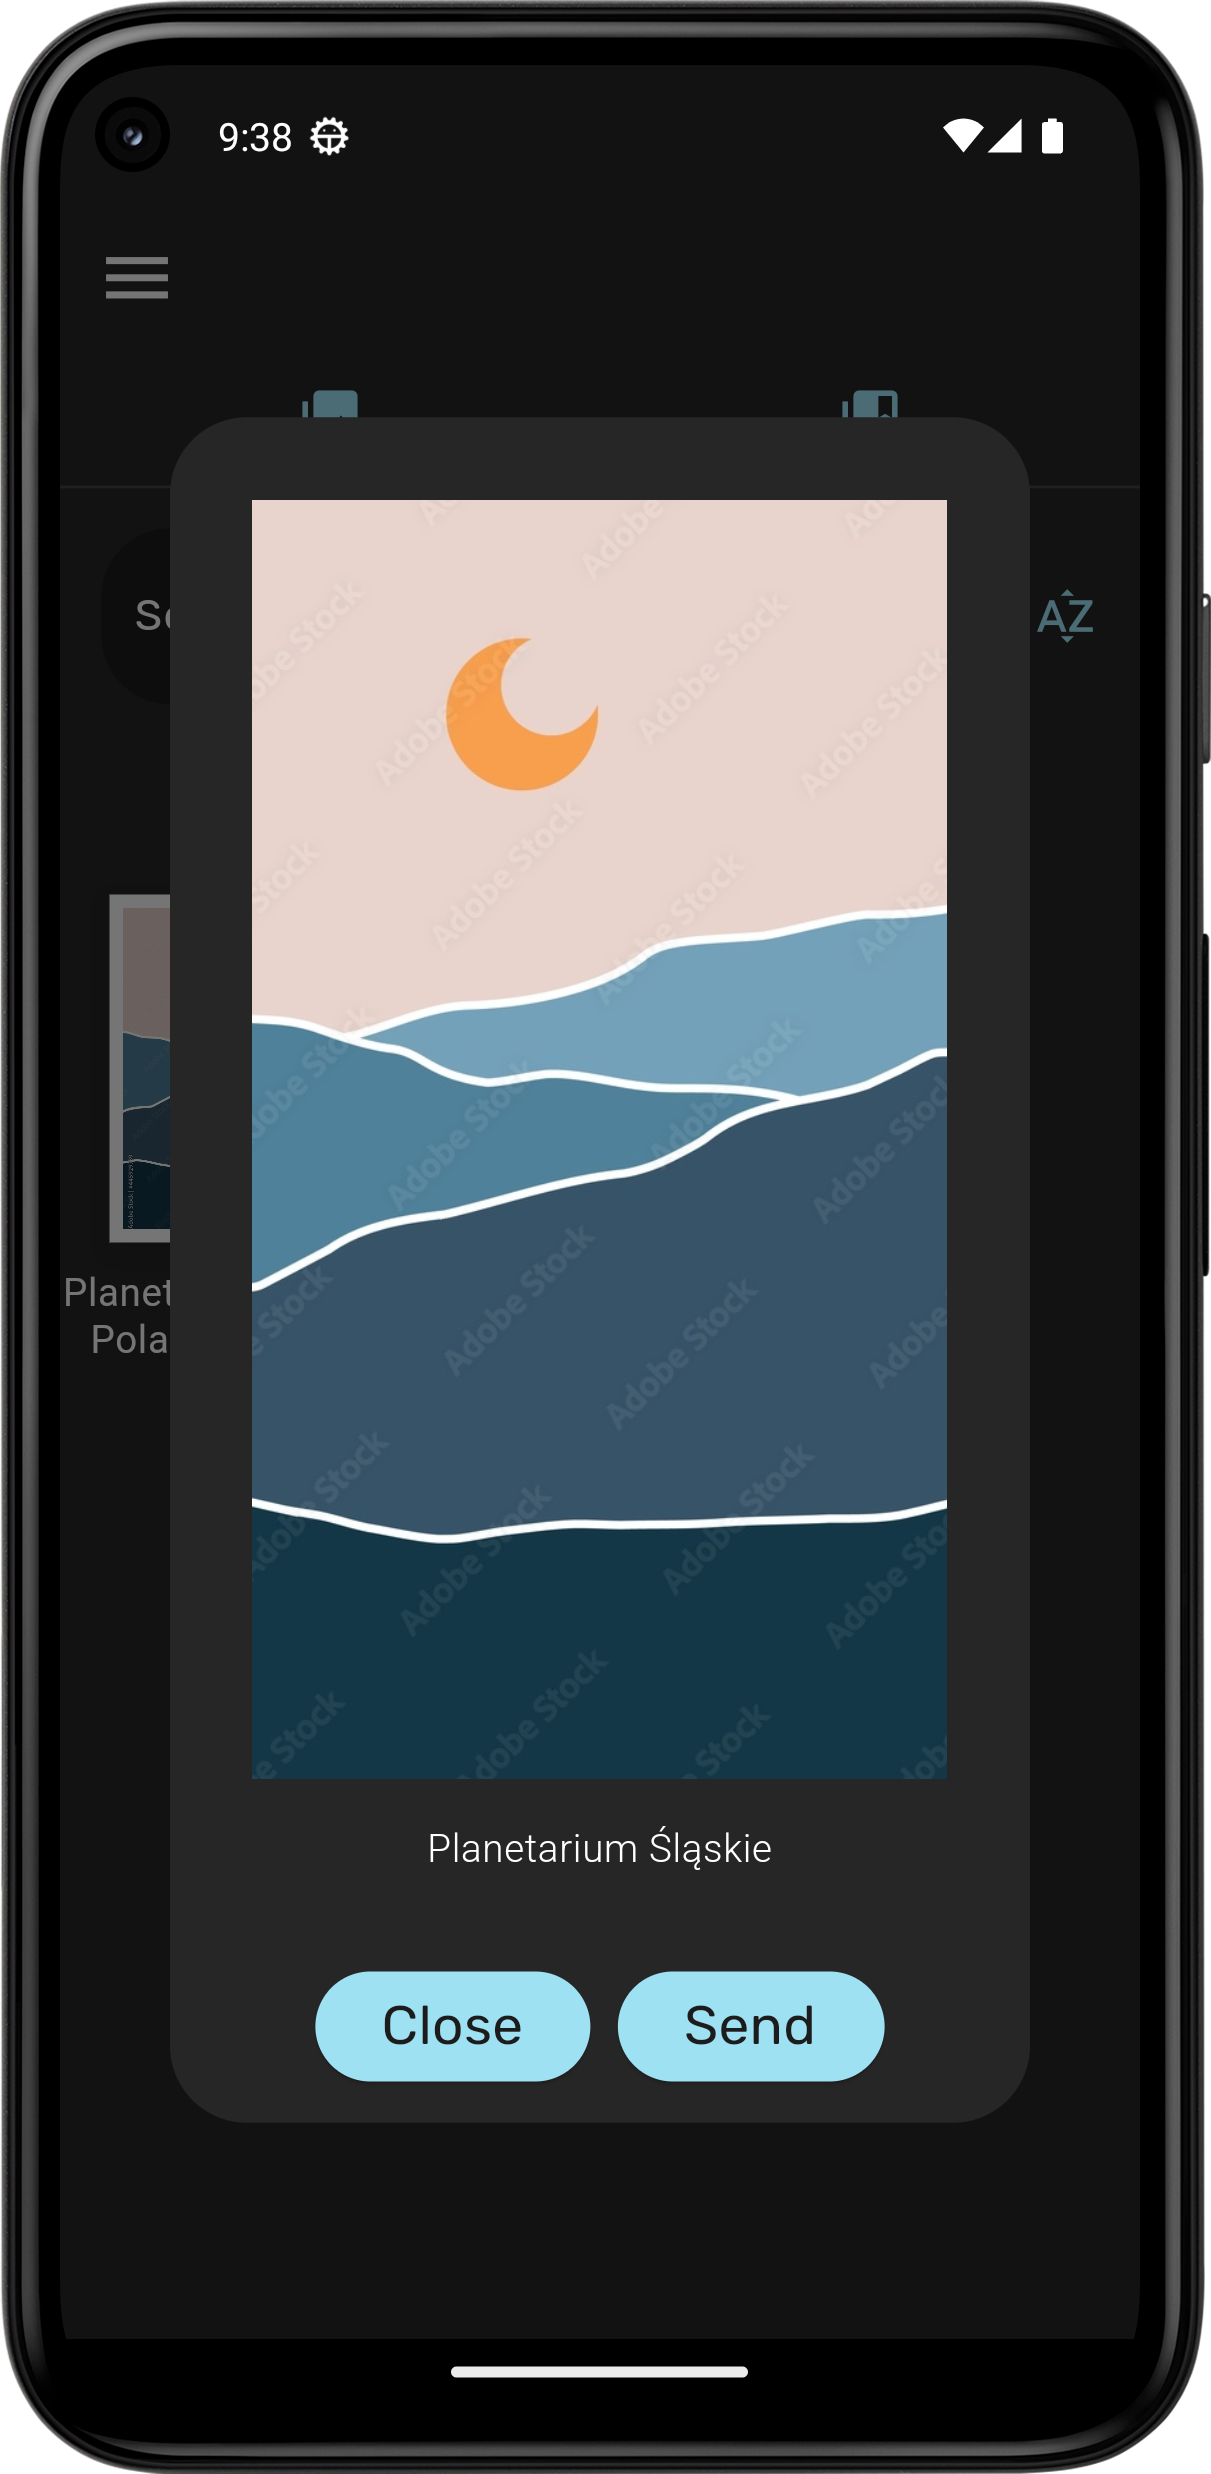
\includegraphics[width=\textwidth]{mobile_ss/pocztowki_podglad.png}
    \caption{Podgląd pocztówki do wysłania}
  \end{minipage}
\end{figure}

Druga zakładka zawiera pocztówki, które dostaliśmy od innych użytkowników. Zawartość jest podobna jak w pierwszej zakładce z tą różnicą, że pocztówki, które są naszymi ulubionymi posiadają złotą ramkę. Różnice znajdują się również w podglądzie. Zamiast przycisku ``Send'' mamy przycisk serduszka, dodający daną pocztówkę do naszych ulubionych.  W podglądzie mamy również tytuł oraz treść, którą ktoś wraz z daną pocztówką nam wysłał.

\begin{figure}[H]
  \centering
  \begin{minipage}[b]{0.49\textwidth}
    \includegraphics[width=\textwidth]{mobile_ss/pocztówki_odebrane.png}
    \caption{Zawartość zakładki z odebranymi pocztówkami}
  \end{minipage}
  \hfill
  \begin{minipage}[b]{0.49\textwidth}
    \includegraphics[width=\textwidth]{mobile_ss/pocztówki_odebrane_podglad.png}
    \caption{Podgląd odebranej pocztówki\\}
  \end{minipage}
\end{figure}

\subsection{Odbieranie pocztówek}

Odbieranie pocztówek następuje na podstronie ``Collect''. Strona posiada dwie listy: pierwsza pokazuje nam pocztówki znajdujące się w zasięgu zebrania, druga natomiast pocztówki znajdujące się w zasięgu powiadamiania, który został ustawiony w opcjach. Gdy wciśniemy przycisk ``Redeem postcard'' na pocztówce z pierwszej listy, do naszej kolekcji dodana zostanie pocztówka dla nas oraz kopia do wysłania naszemu znajomemu. Gdy wciśniemy pocztówkę znajdującą się w drugiej liście, zostaniemy przeniesieni do strony pokazującej nam dokładne koordynaty pocztówki, jak i przycisk, który przeniesie nas do strony Google Maps z ustawioną już pocztówką do danej lokalizacji.

\begin{figure}[H]
  \centering
  \begin{minipage}[b]{0.49\textwidth}
    \includegraphics[width=\textwidth]{mobile_ss/odbieranie pocztówek.png}
    \caption{Podstrona do odbierania pocztówek}
  \end{minipage}
  \hfill
  \begin{minipage}[b]{0.49\textwidth}
    \includegraphics[width=\textwidth]{mobile_ss/lokalizownaie_pocztówki.png}
    \caption{Podstrona do lokalizowania pocztówki}
  \end{minipage}
\end{figure}

Aplikacja posiada również mechanizm powiadamiania użytkownika o tym, że znajduje się w pobliżu pocztówki do odebrania. Gdy znajdujemy się w jej zasięgu zostaje wysłane lokalne powiadomienie. Jest one wysyłane tylko raz na godzinę lub do momentu ponownego włączenia lokalizowania pocztówek.

\begin{figure}[H]
    \centering
    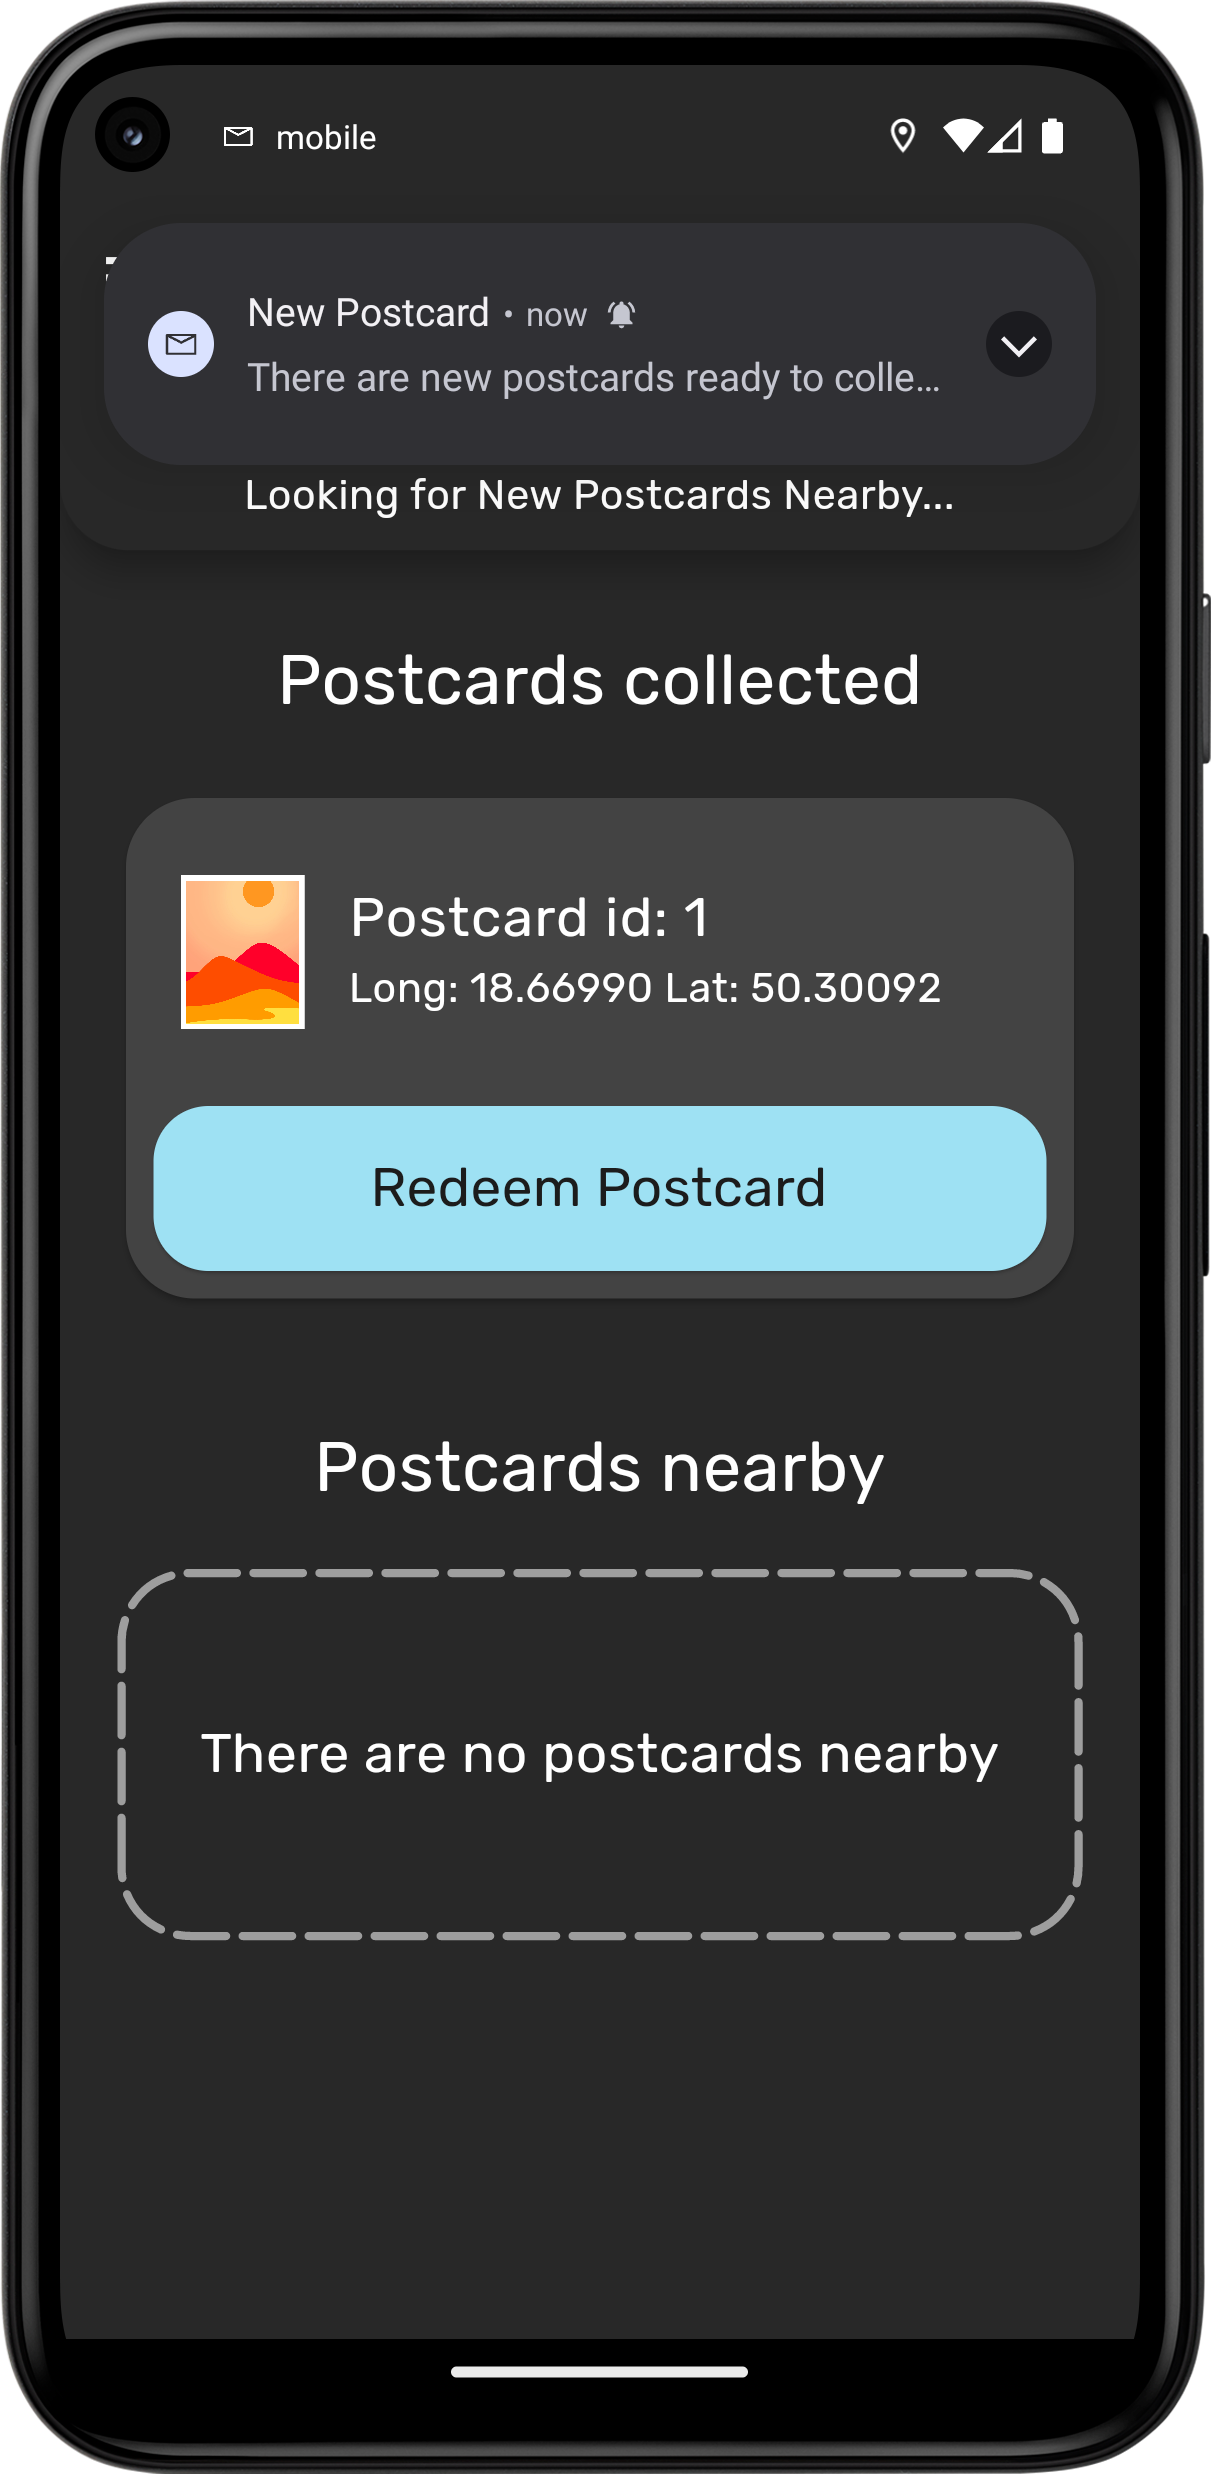
\includegraphics[width=0.5\textwidth]{mobile_ss/powiadomienie.png}
    \caption{Powiadomienie o nowej pocztówce}
\end{figure}

Podstrona do odbioru pocztówek posiada również wersję, gdy użytkownik nie włączył lokalizowania pocztówek jak i również wersje, gdy lokalizacja jest w telefonie całkowicie wyłączona.

\begin{figure}[H]
  \centering
  \begin{minipage}[b]{0.49\textwidth}
    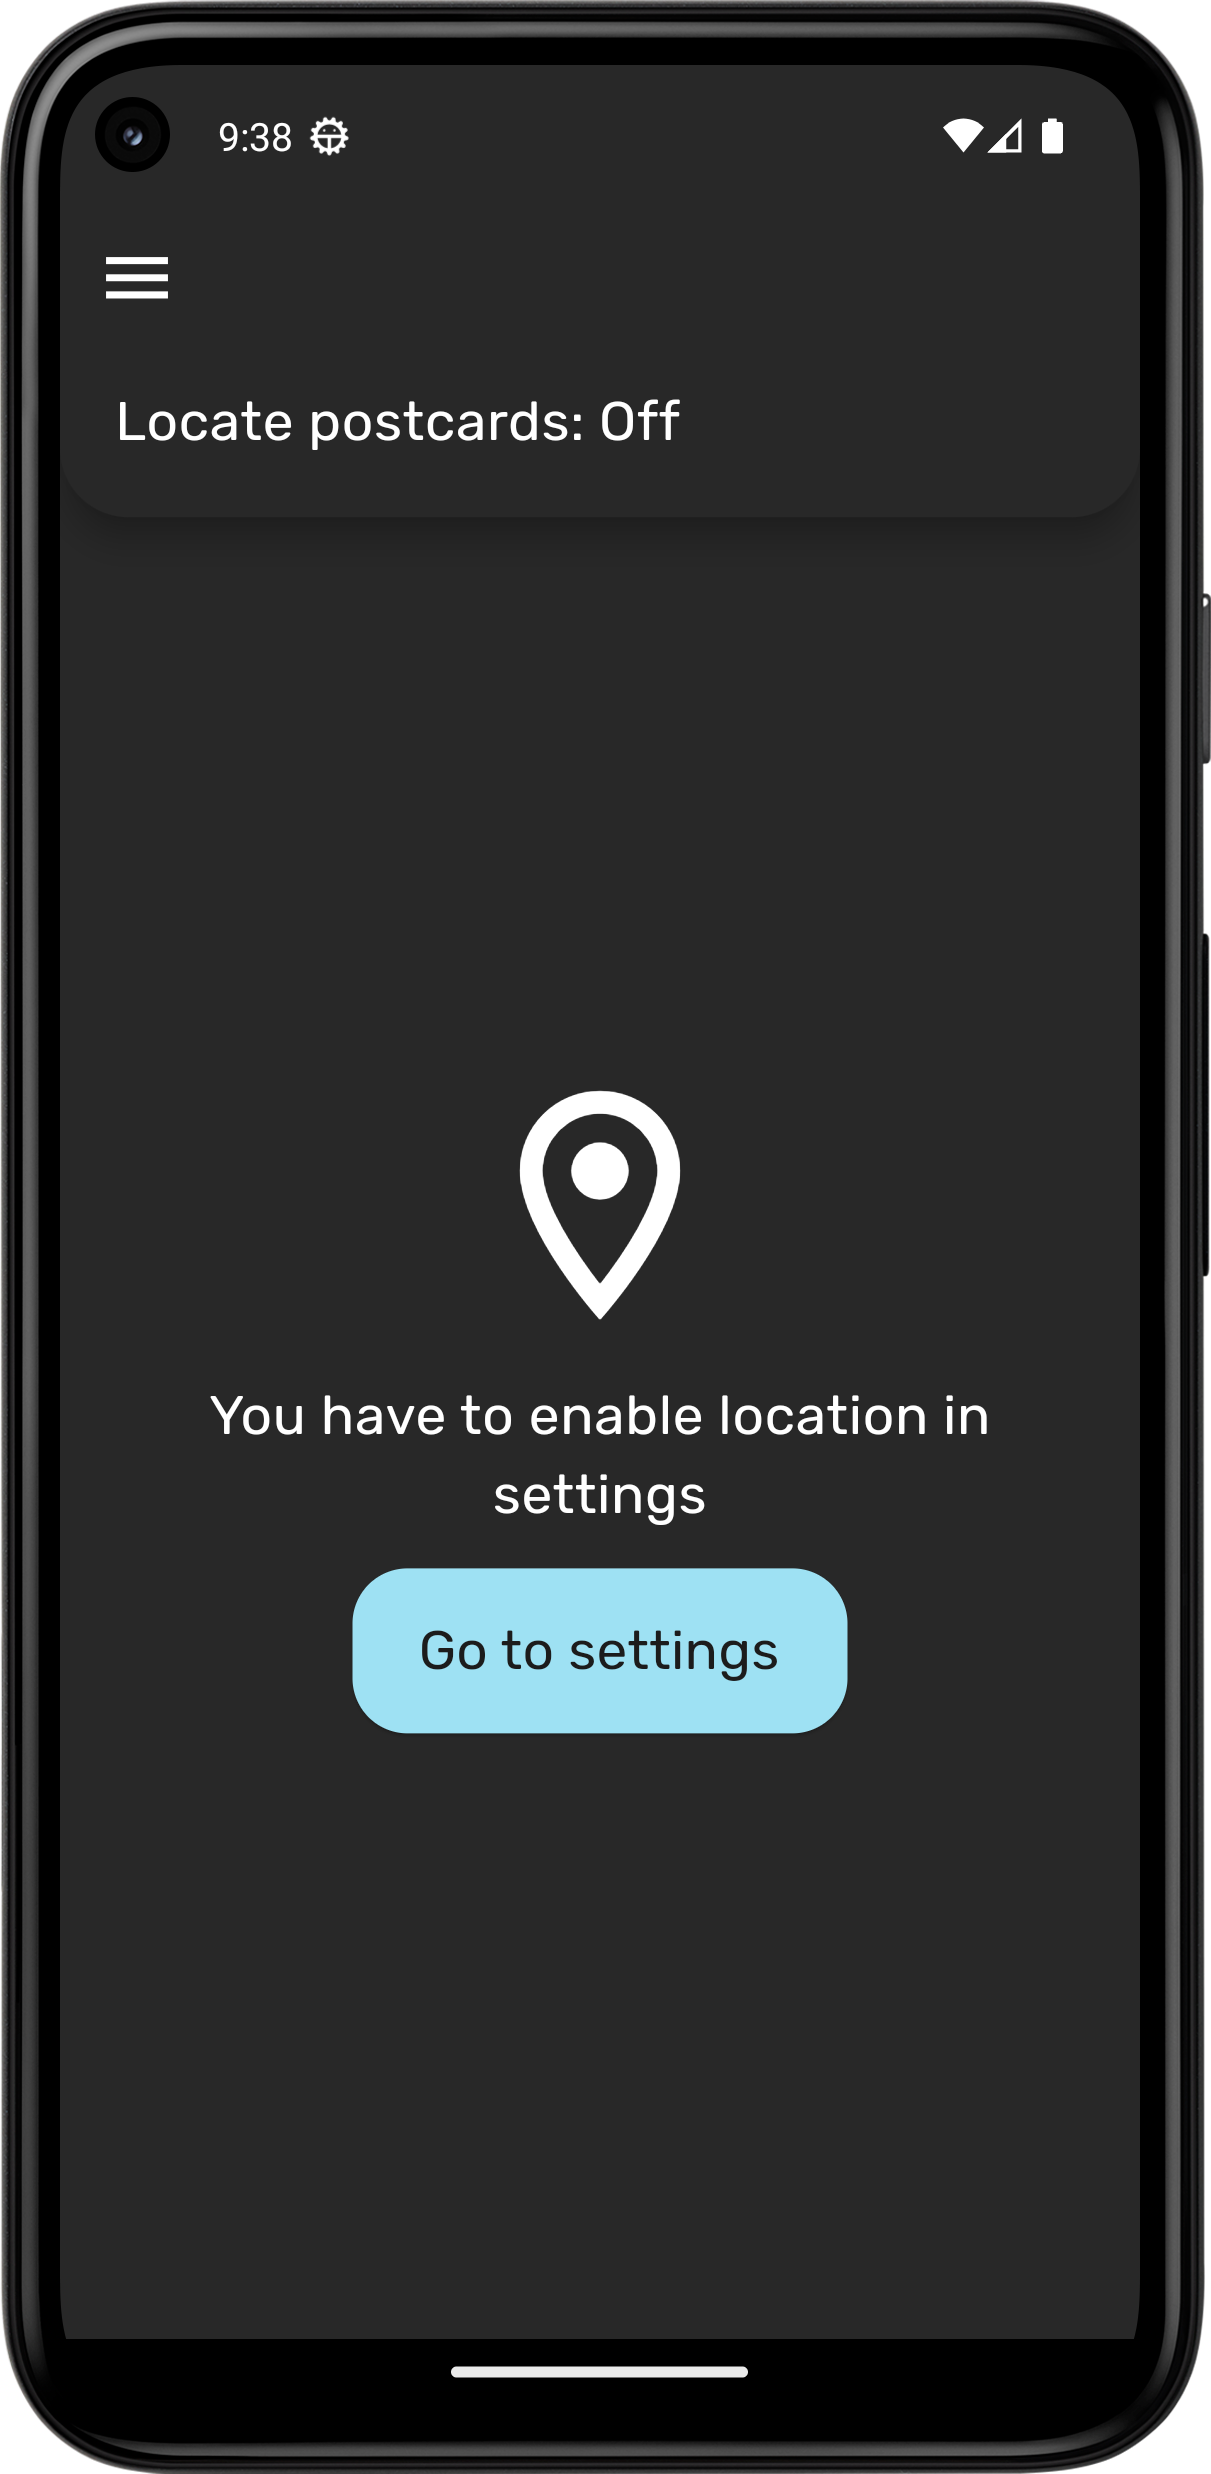
\includegraphics[width=\textwidth]{mobile_ss/lokalizacja_pocztowek_wylaczana.png}
    \caption{Wersja podstrony gdy lokalizowanie pocztówek jest wyłączone}
  \end{minipage}
  \hfill
  \begin{minipage}[b]{0.49\textwidth}
    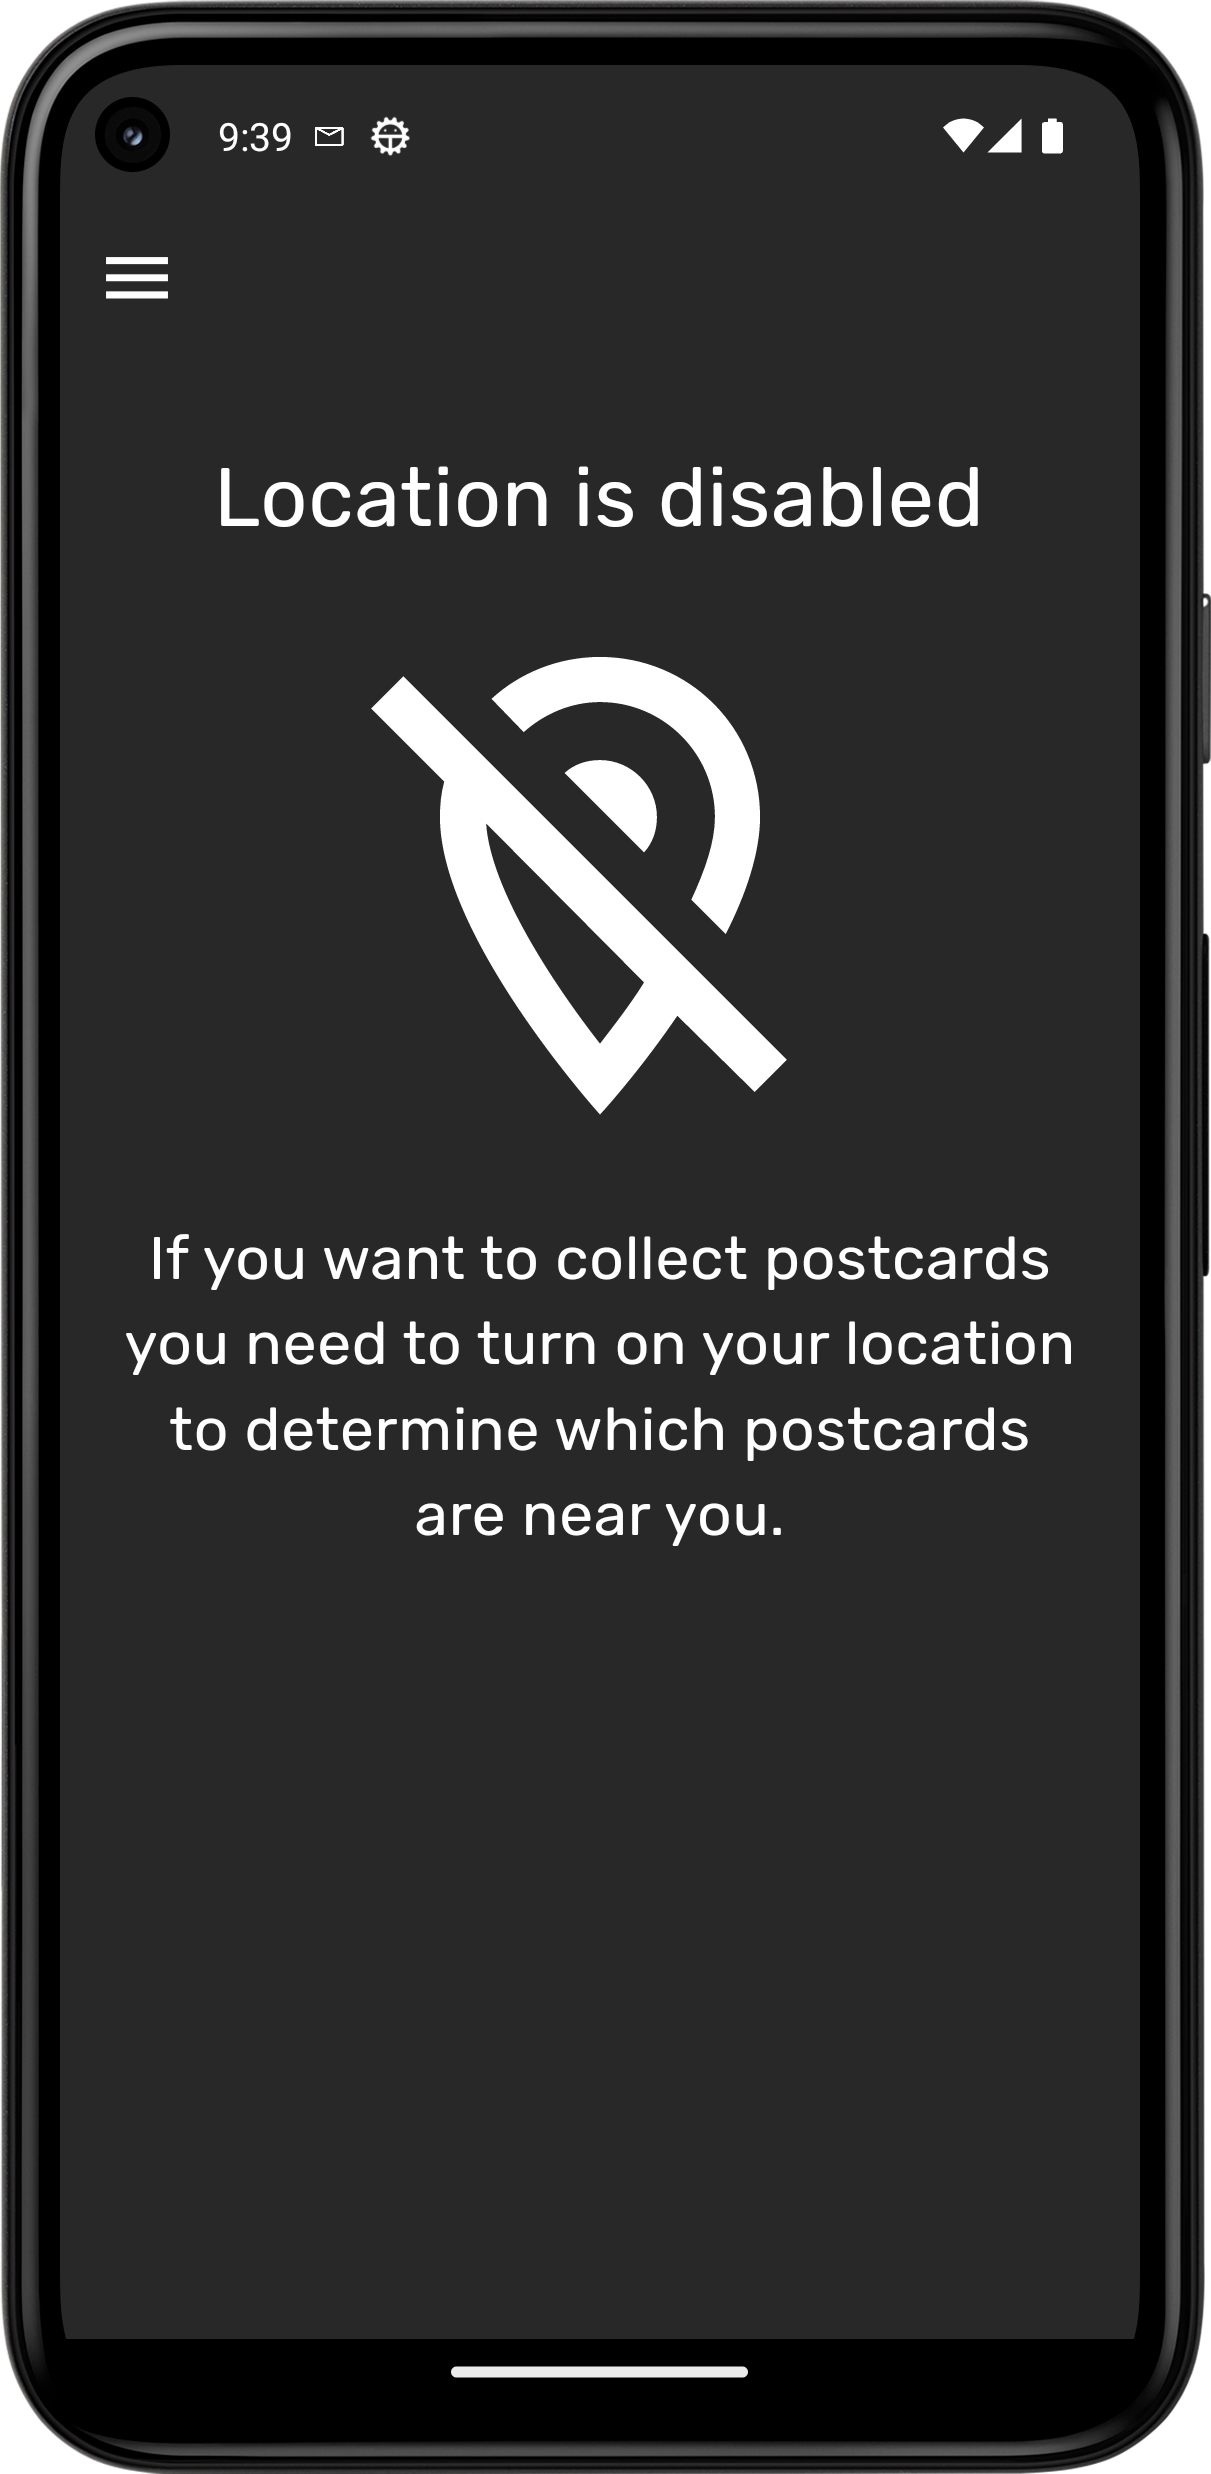
\includegraphics[width=\textwidth]{mobile_ss/lokalizacja_w_tel_wylaczana.png}
    \caption{Wersja podstrony gdy lokalizacja w telefonie jest wyłączona}
  \end{minipage}
\end{figure}

\subsection{Ustawienia}
W ustawieniach, użytkownik może dostosować aplikację do swoich potrzeb jak i zarządzać pewnymi jej funkcjami. 
Ustawienia umożliwiają:
\begin{itemize}
    \item Zmieniać motyw na jasny lub ciemny.
    \item Włączać i wyłączać lokalizowanie pocztówek.
    \item Włączać i wyłączać powiadomienia.
    \item Zmieniać zasięg powiadamiania użytkownika o pocztówkach w pobliżu.
    \item Zmieniać format daty.
    \item Zmieniać typ jednostek.
    \item Przeczytanie zasad korzystania z aplikacji.
    \item Usunięcie konta.
\end{itemize}

\begin{figure}[H]
    \centering
    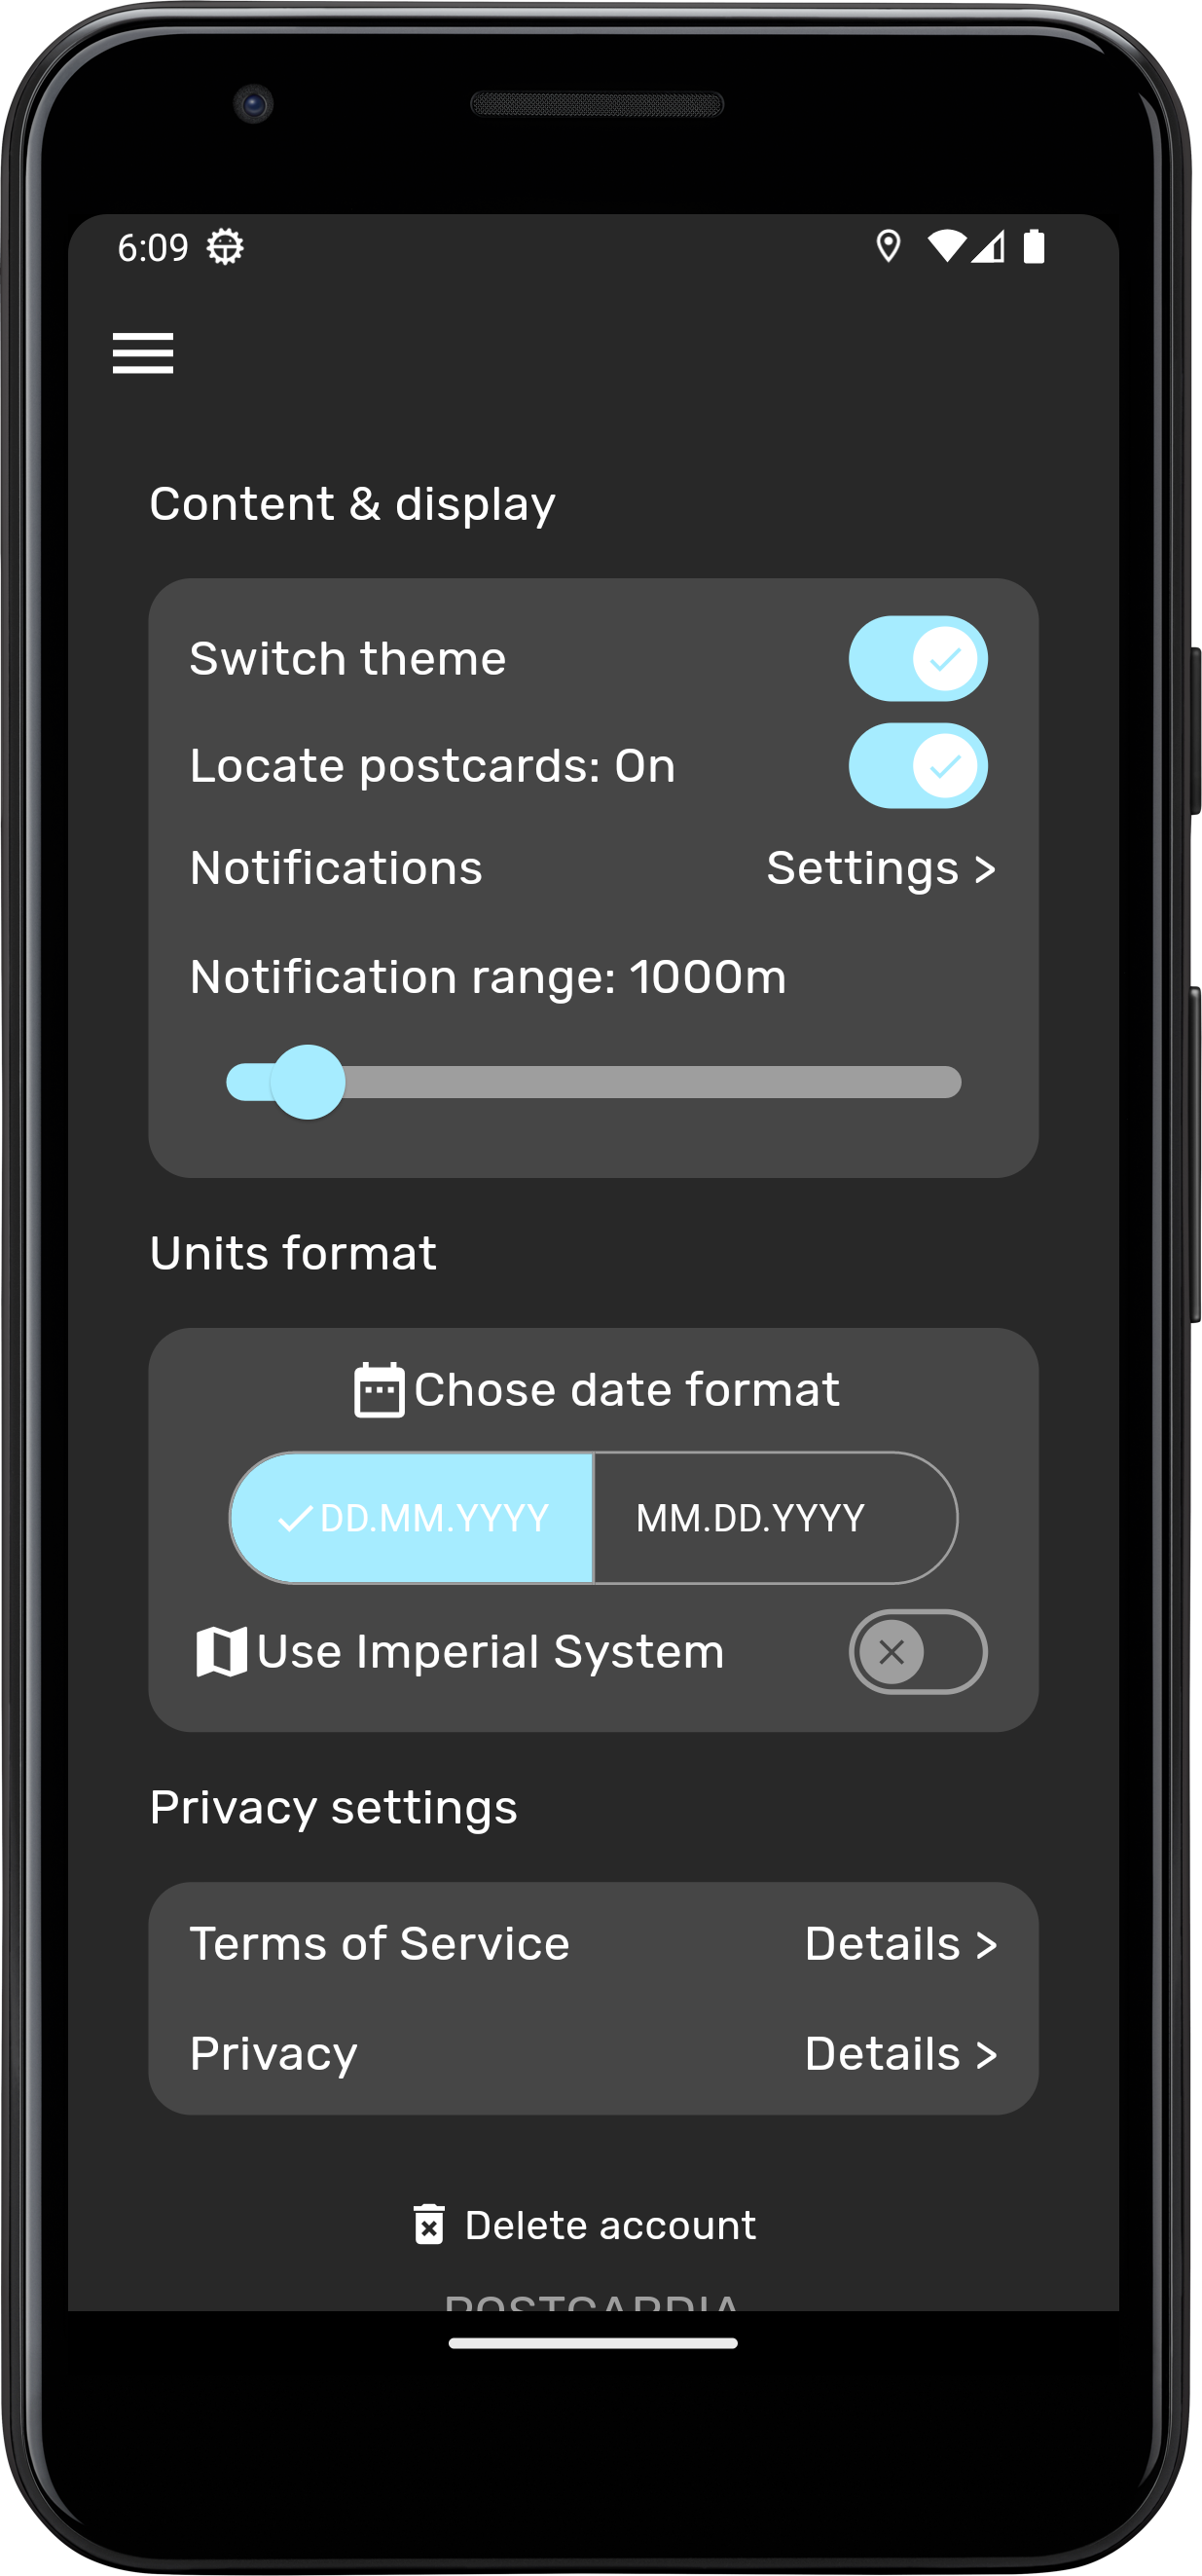
\includegraphics[width=0.5\textwidth]{mobile_ss/ustawienia.png}
    \caption{Podstrona z ustawieniami}
\end{figure}

\subsection{Panel administratora}
Użytkownicy ze statusem administratora mają dostęp do dodatkowej zakładki, w której mogą edytować istniejące już pocztówki jak i również z poziomu aplikacji dodawać nowe. Przeglądanie pocztówek w panelu admina jest wykonane podobnie do przeglądania pocztówek zwykłego użytkownika.

\begin{figure}[H]
  \centering
  \begin{minipage}[b]{0.49\textwidth}
    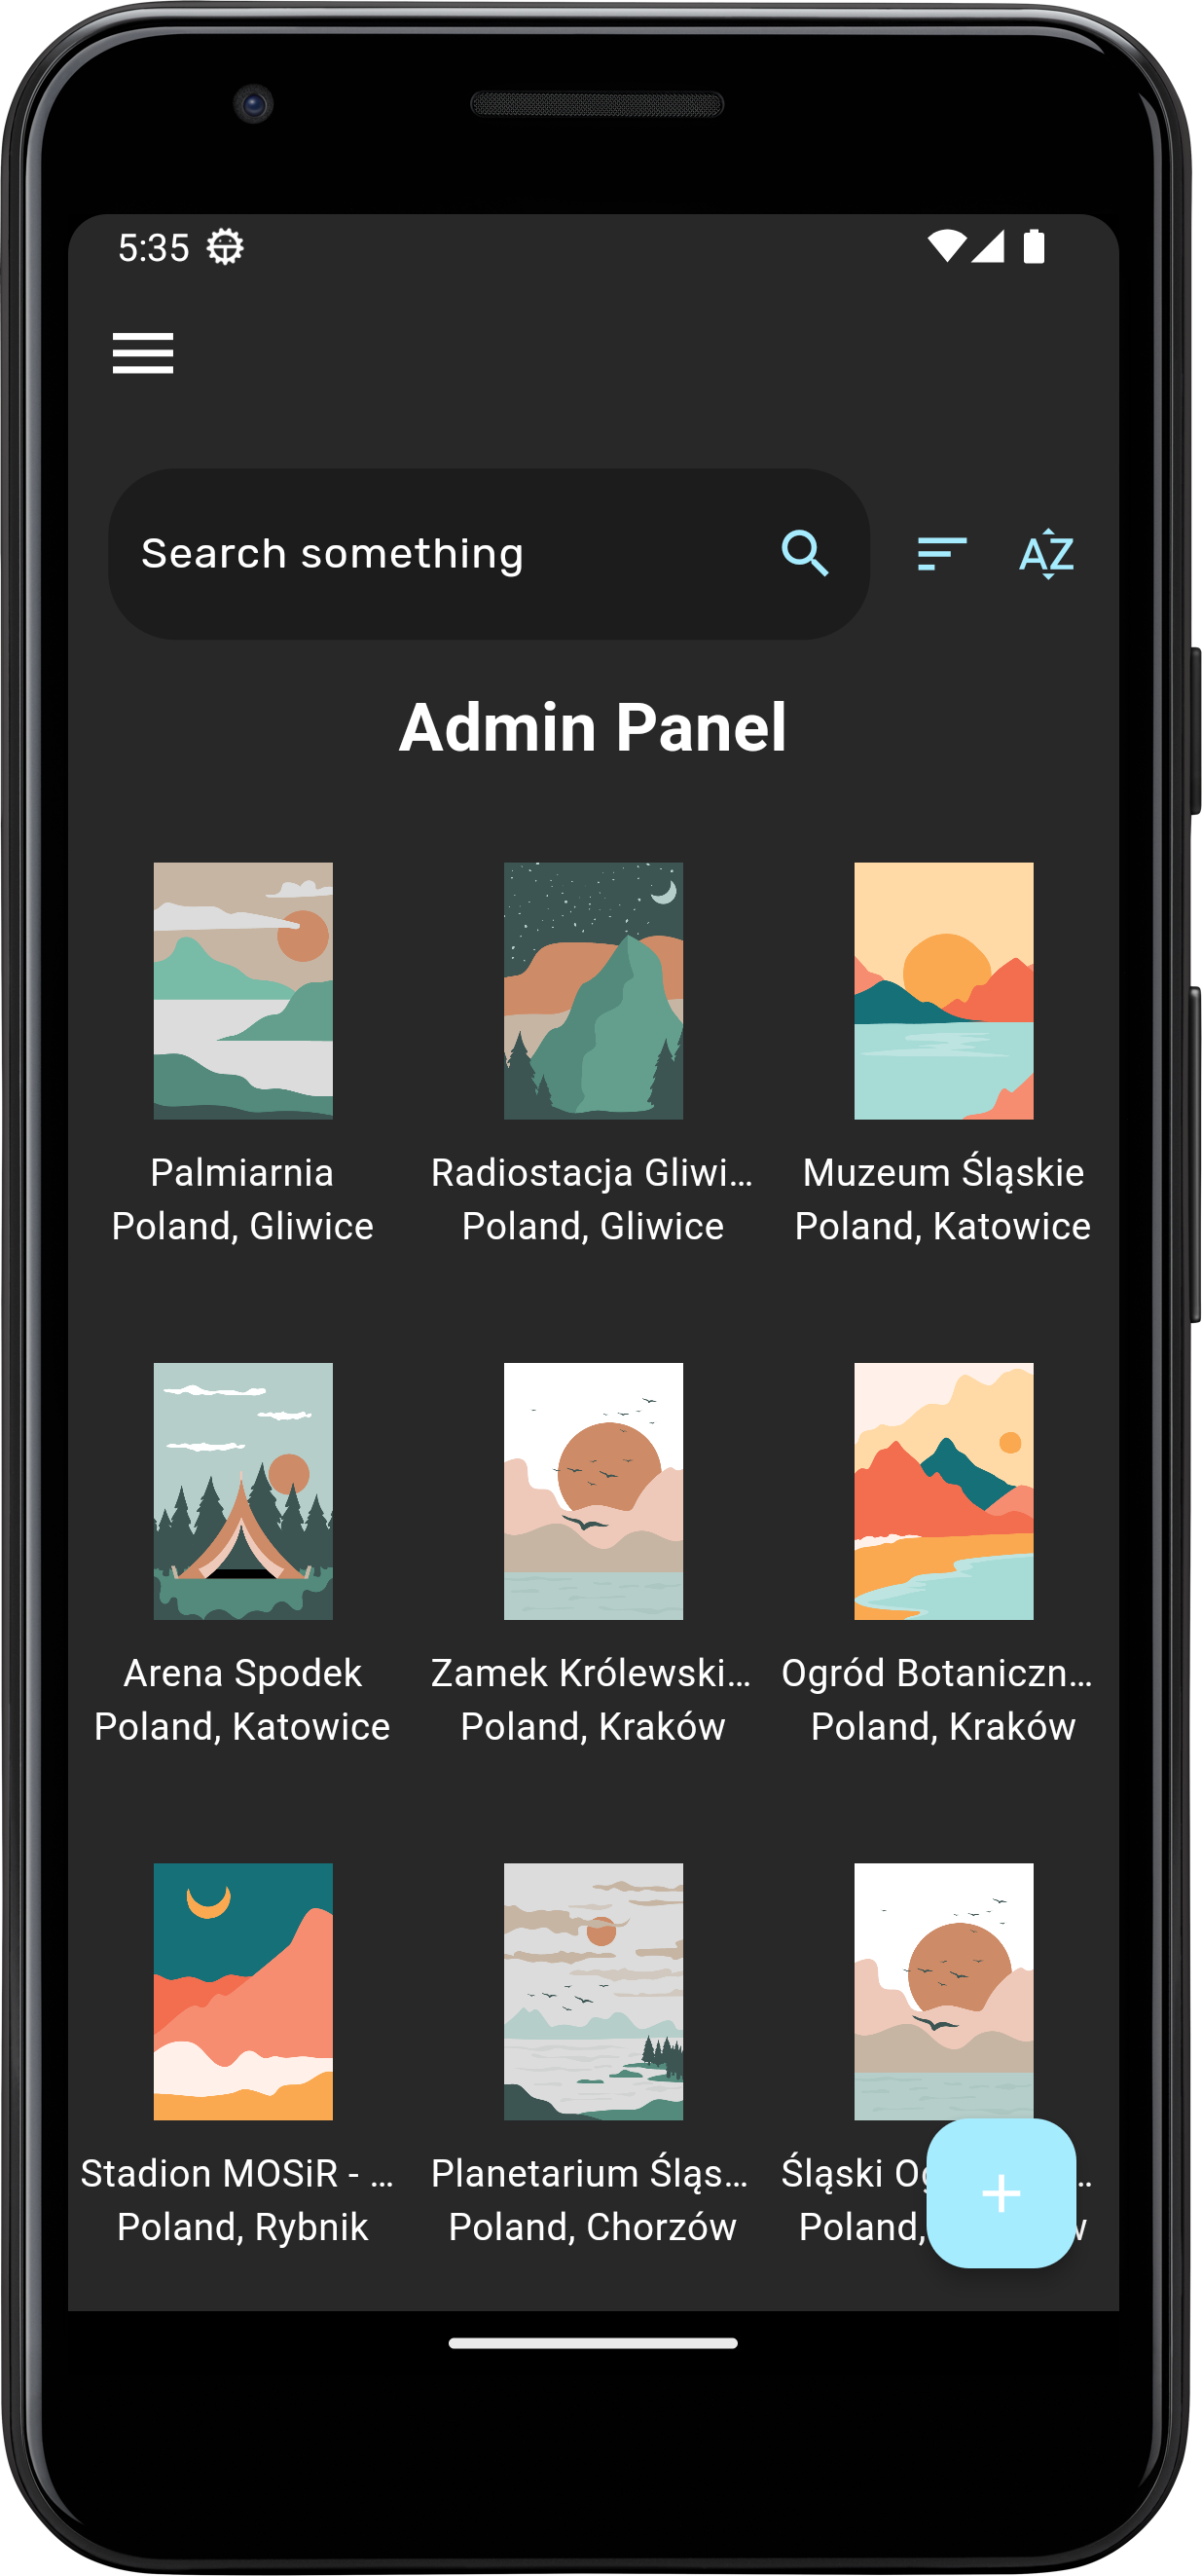
\includegraphics[width=\textwidth]{mobile_ss/admin.png}
    \caption{Podstrona do zarządzania pocztówkami}
  \end{minipage}
  \hfill
  \begin{minipage}[b]{0.49\textwidth}
    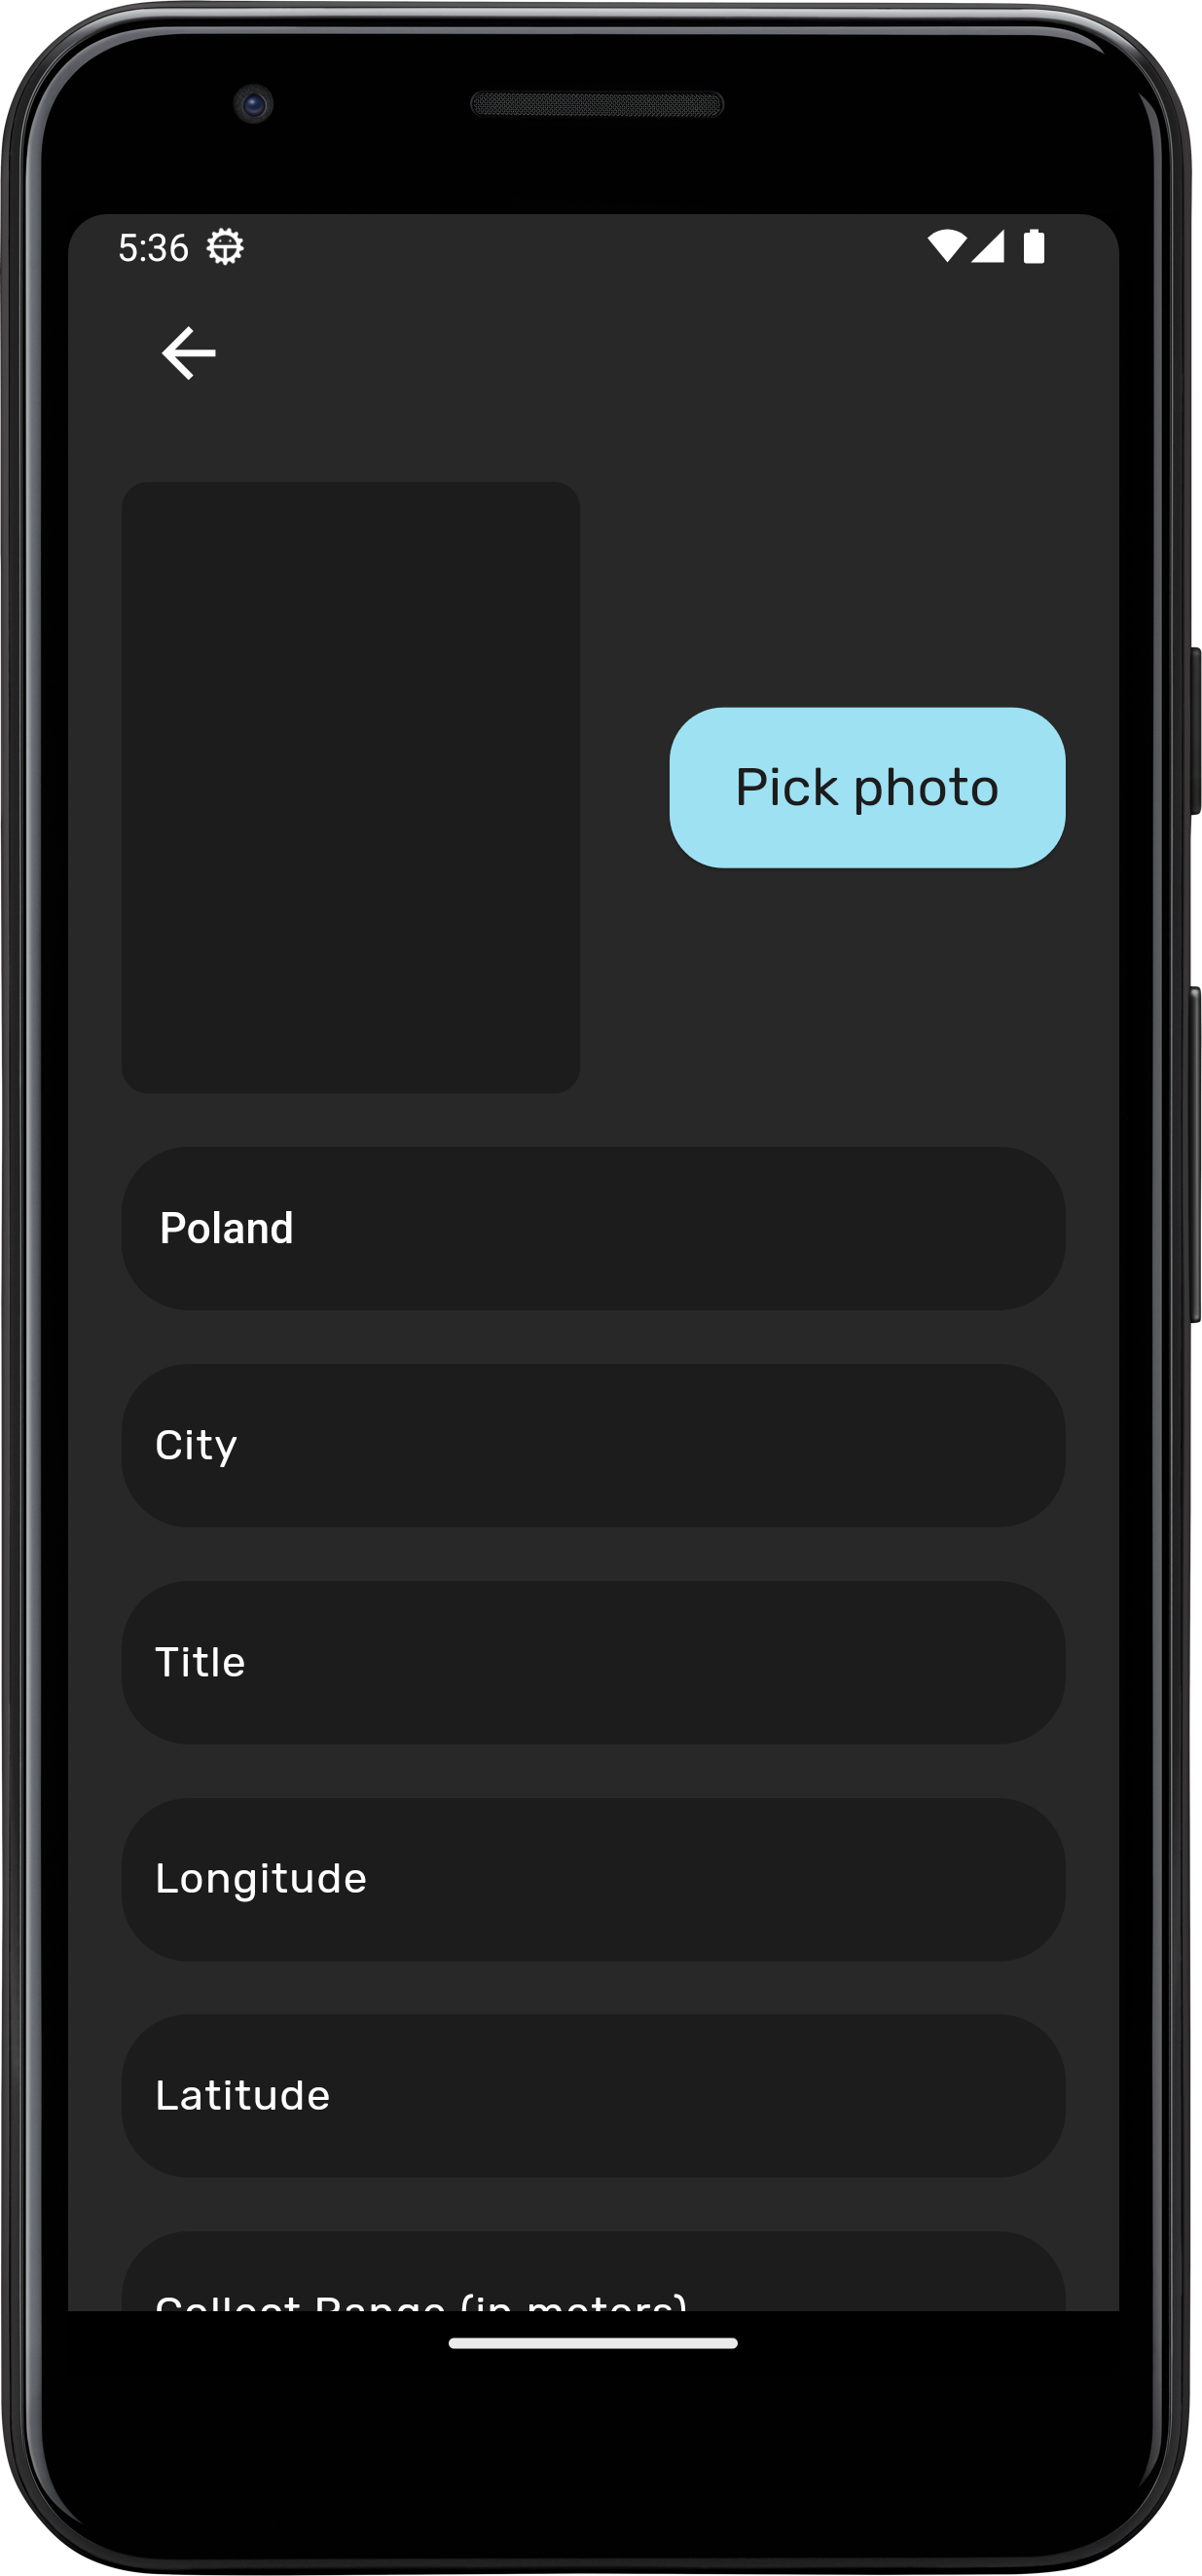
\includegraphics[width=\textwidth]{mobile_ss/admin_edit.png}
    \caption{Podstrona do edycji i dodawania nowych pocztówek}
  \end{minipage}
\end{figure}

\subsection{Znajomi}
Strona która służy do zdobywania nowych znajomości jest podzielona na 3 zakładki. W pierwszej zakładce znajdują się użytkownicy, których śledzimy, w drugiej zakładce znajdują się użytkownicy, którzy nas śledzą, natomiast w trzeciej zakładce znajdują się wszyscy użytkownicy. 

\begin{figure}[H]
  \centering
  \begin{minipage}[b]{0.30\textwidth}
    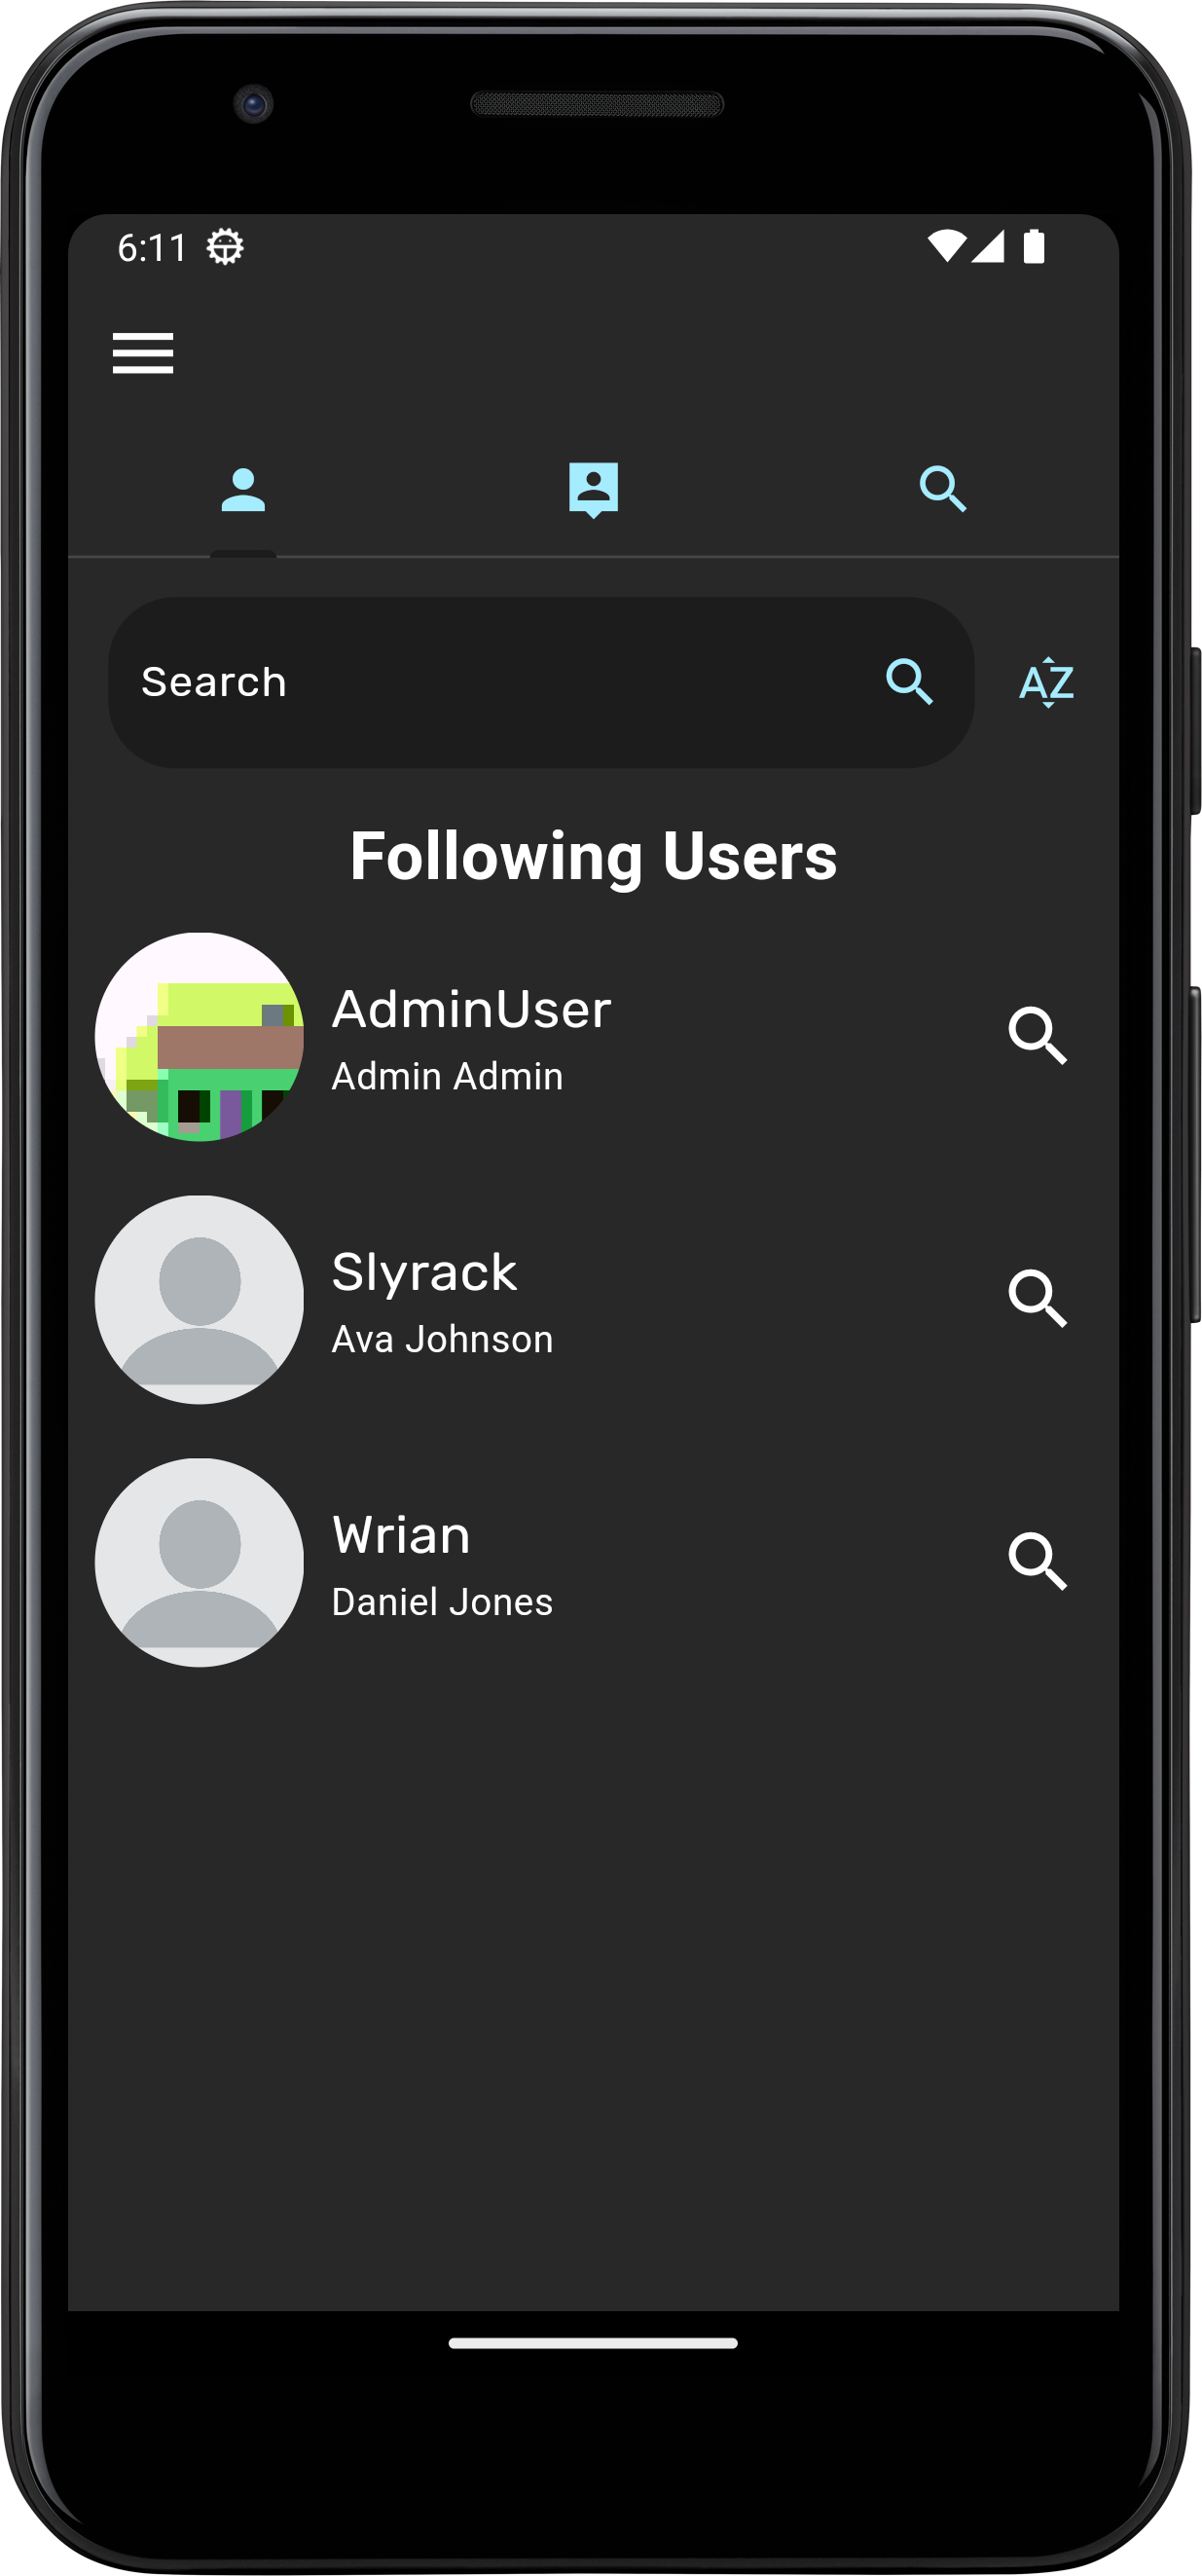
\includegraphics[width=\textwidth]{mobile_ss/followani.png}
    \caption{Zakładka ze śledzonymi użytkownikami\\}
  \end{minipage}
  \hfill
  \begin{minipage}[b]{0.30\textwidth}
    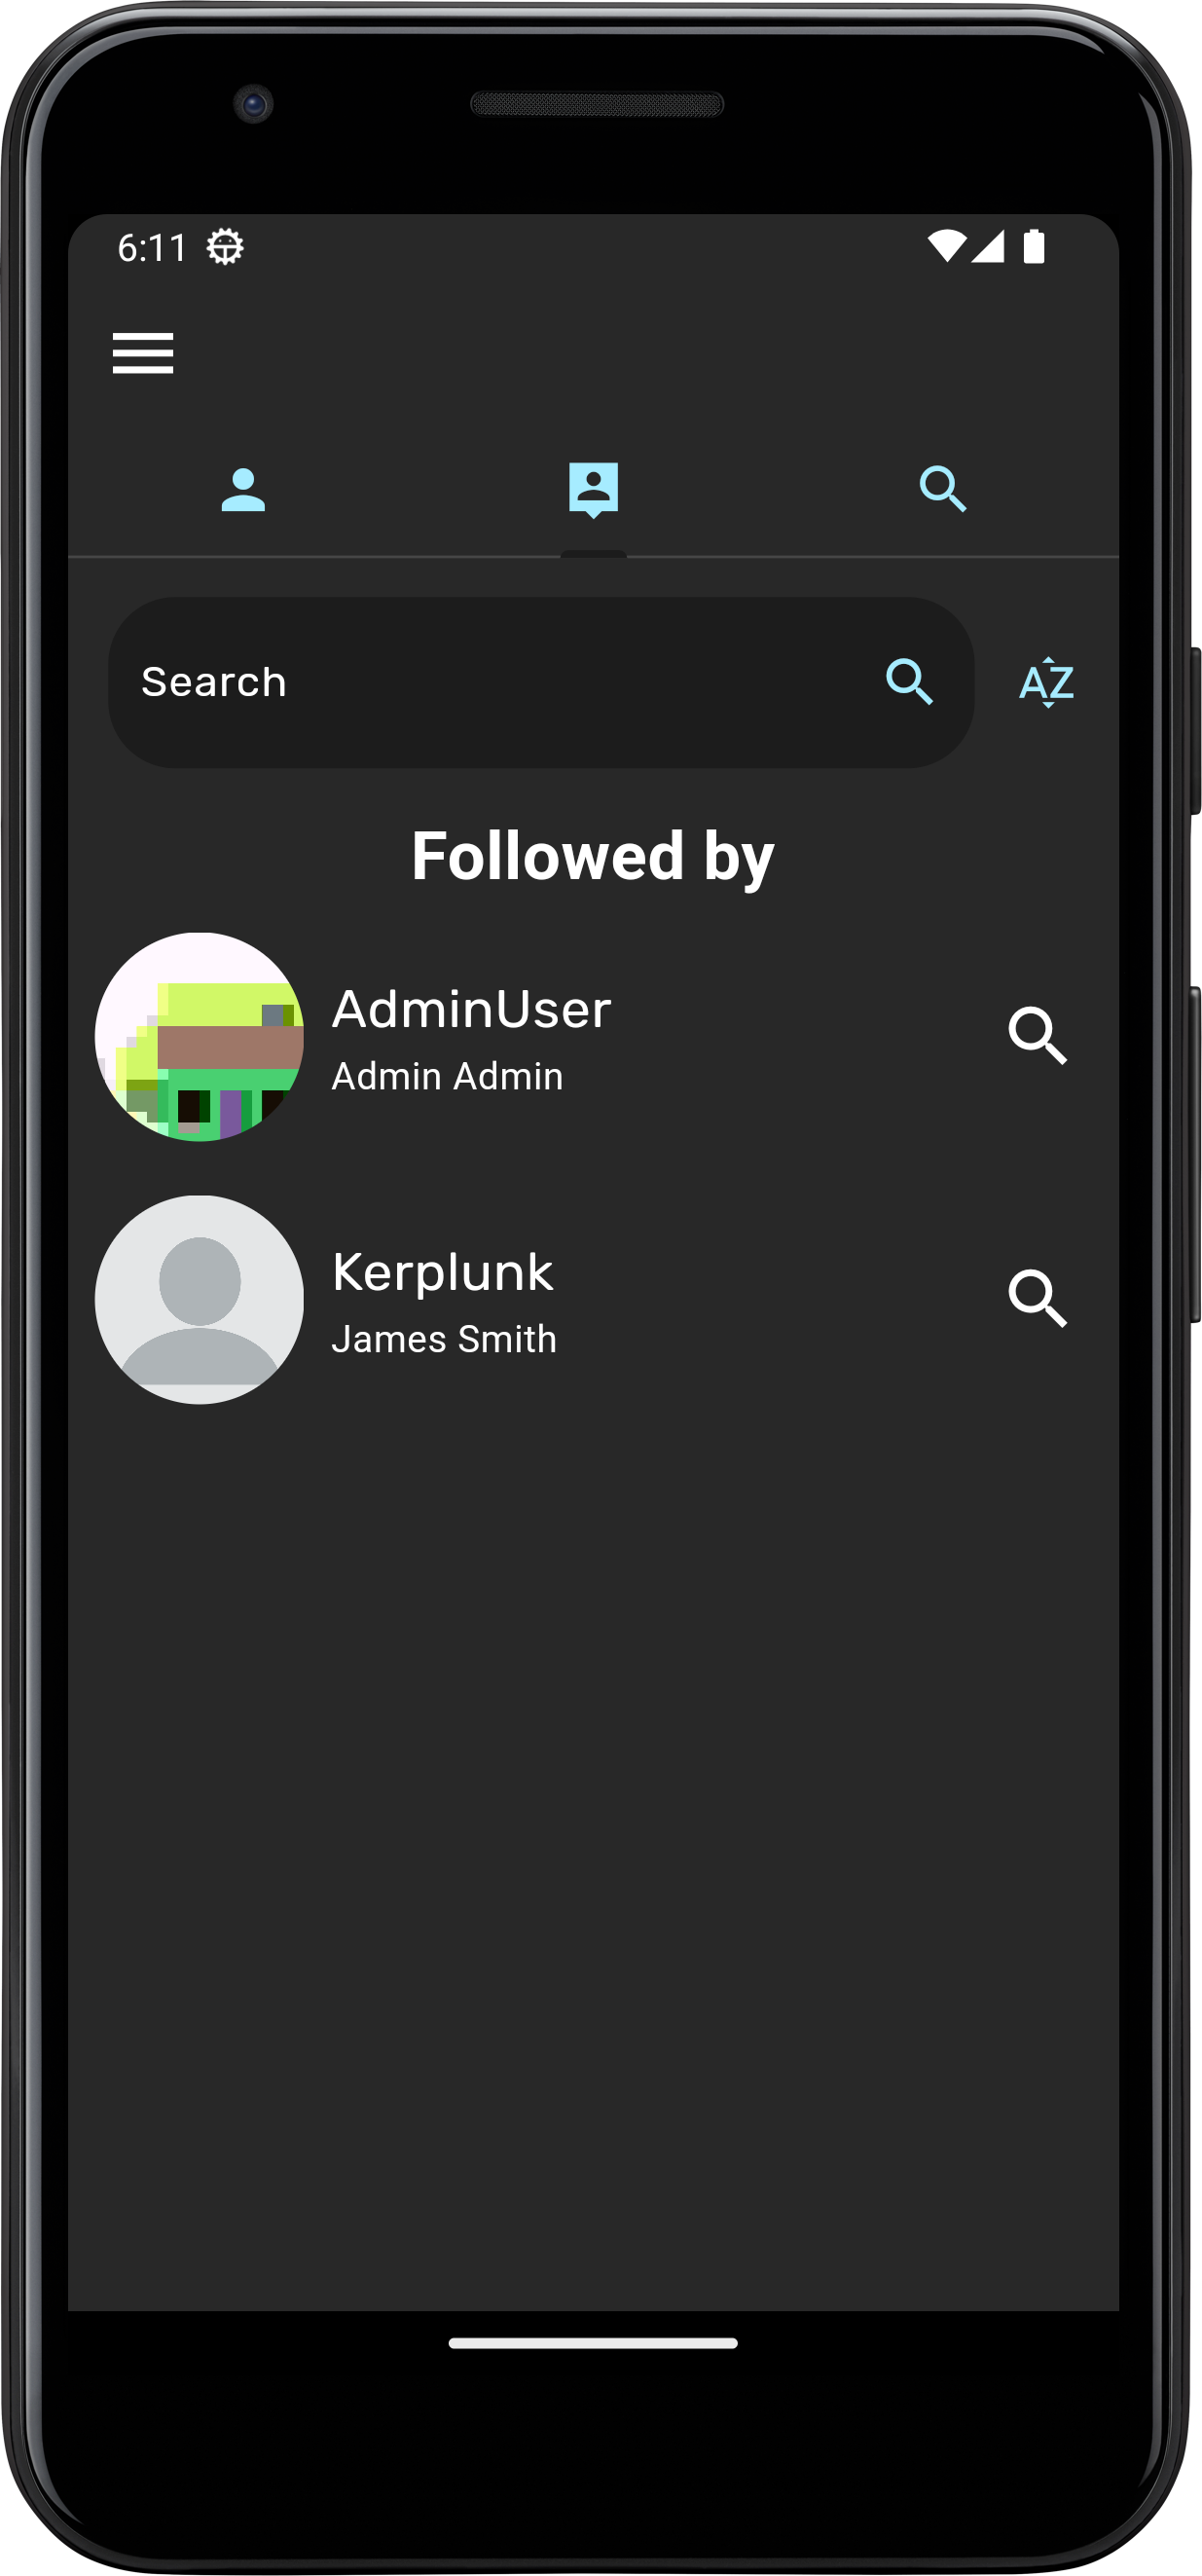
\includegraphics[width=\textwidth]{mobile_ss/followingby.png}
    \caption{Zakładka z użytkownikami którzy nas śledzą}
  \end{minipage}
  \hfill
  \begin{minipage}[b]{0.30\textwidth}
    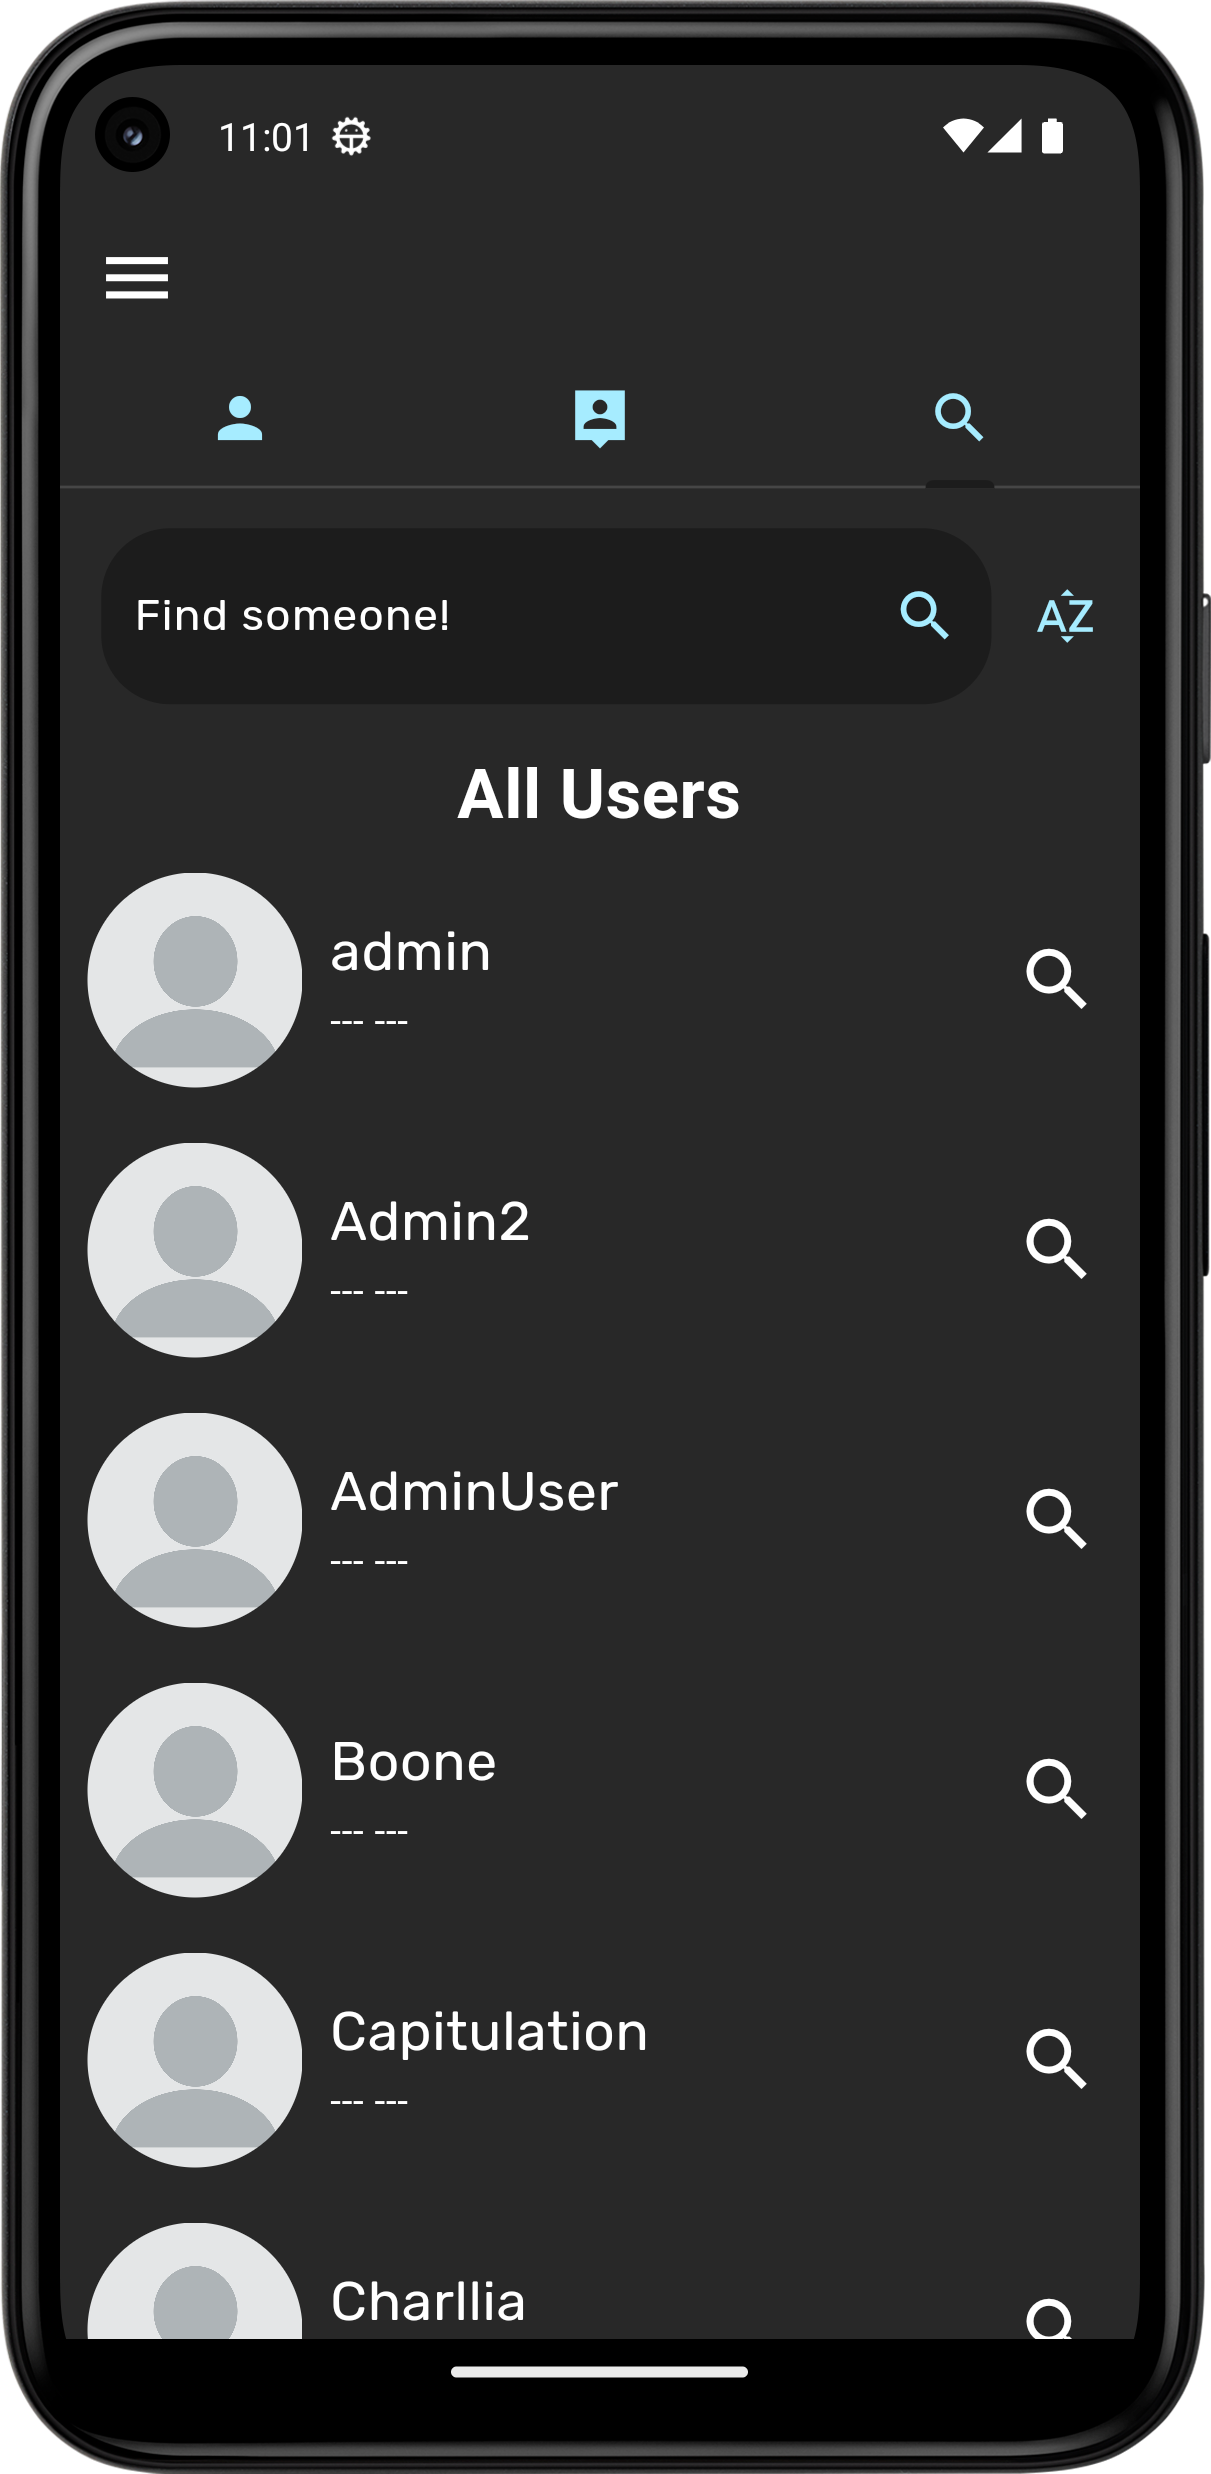
\includegraphics[width=\textwidth]{mobile_ss/wszyscyUzytkownicy.png}
    \caption{Zakładka ze wszystkimi użytkownikami\\}
  \end{minipage}
\end{figure}

Po wciśnięciu na dowolnej zakładce karty z użytkownikiem zostaniemy przekierowani do strony ze szczegółami danego użytkownika, na której również znajduje się przycisk, który służy do śledzenia lub zrezygnowania ze śledzenia danego użytkownika. 

\begin{figure}[H]
    \centering
    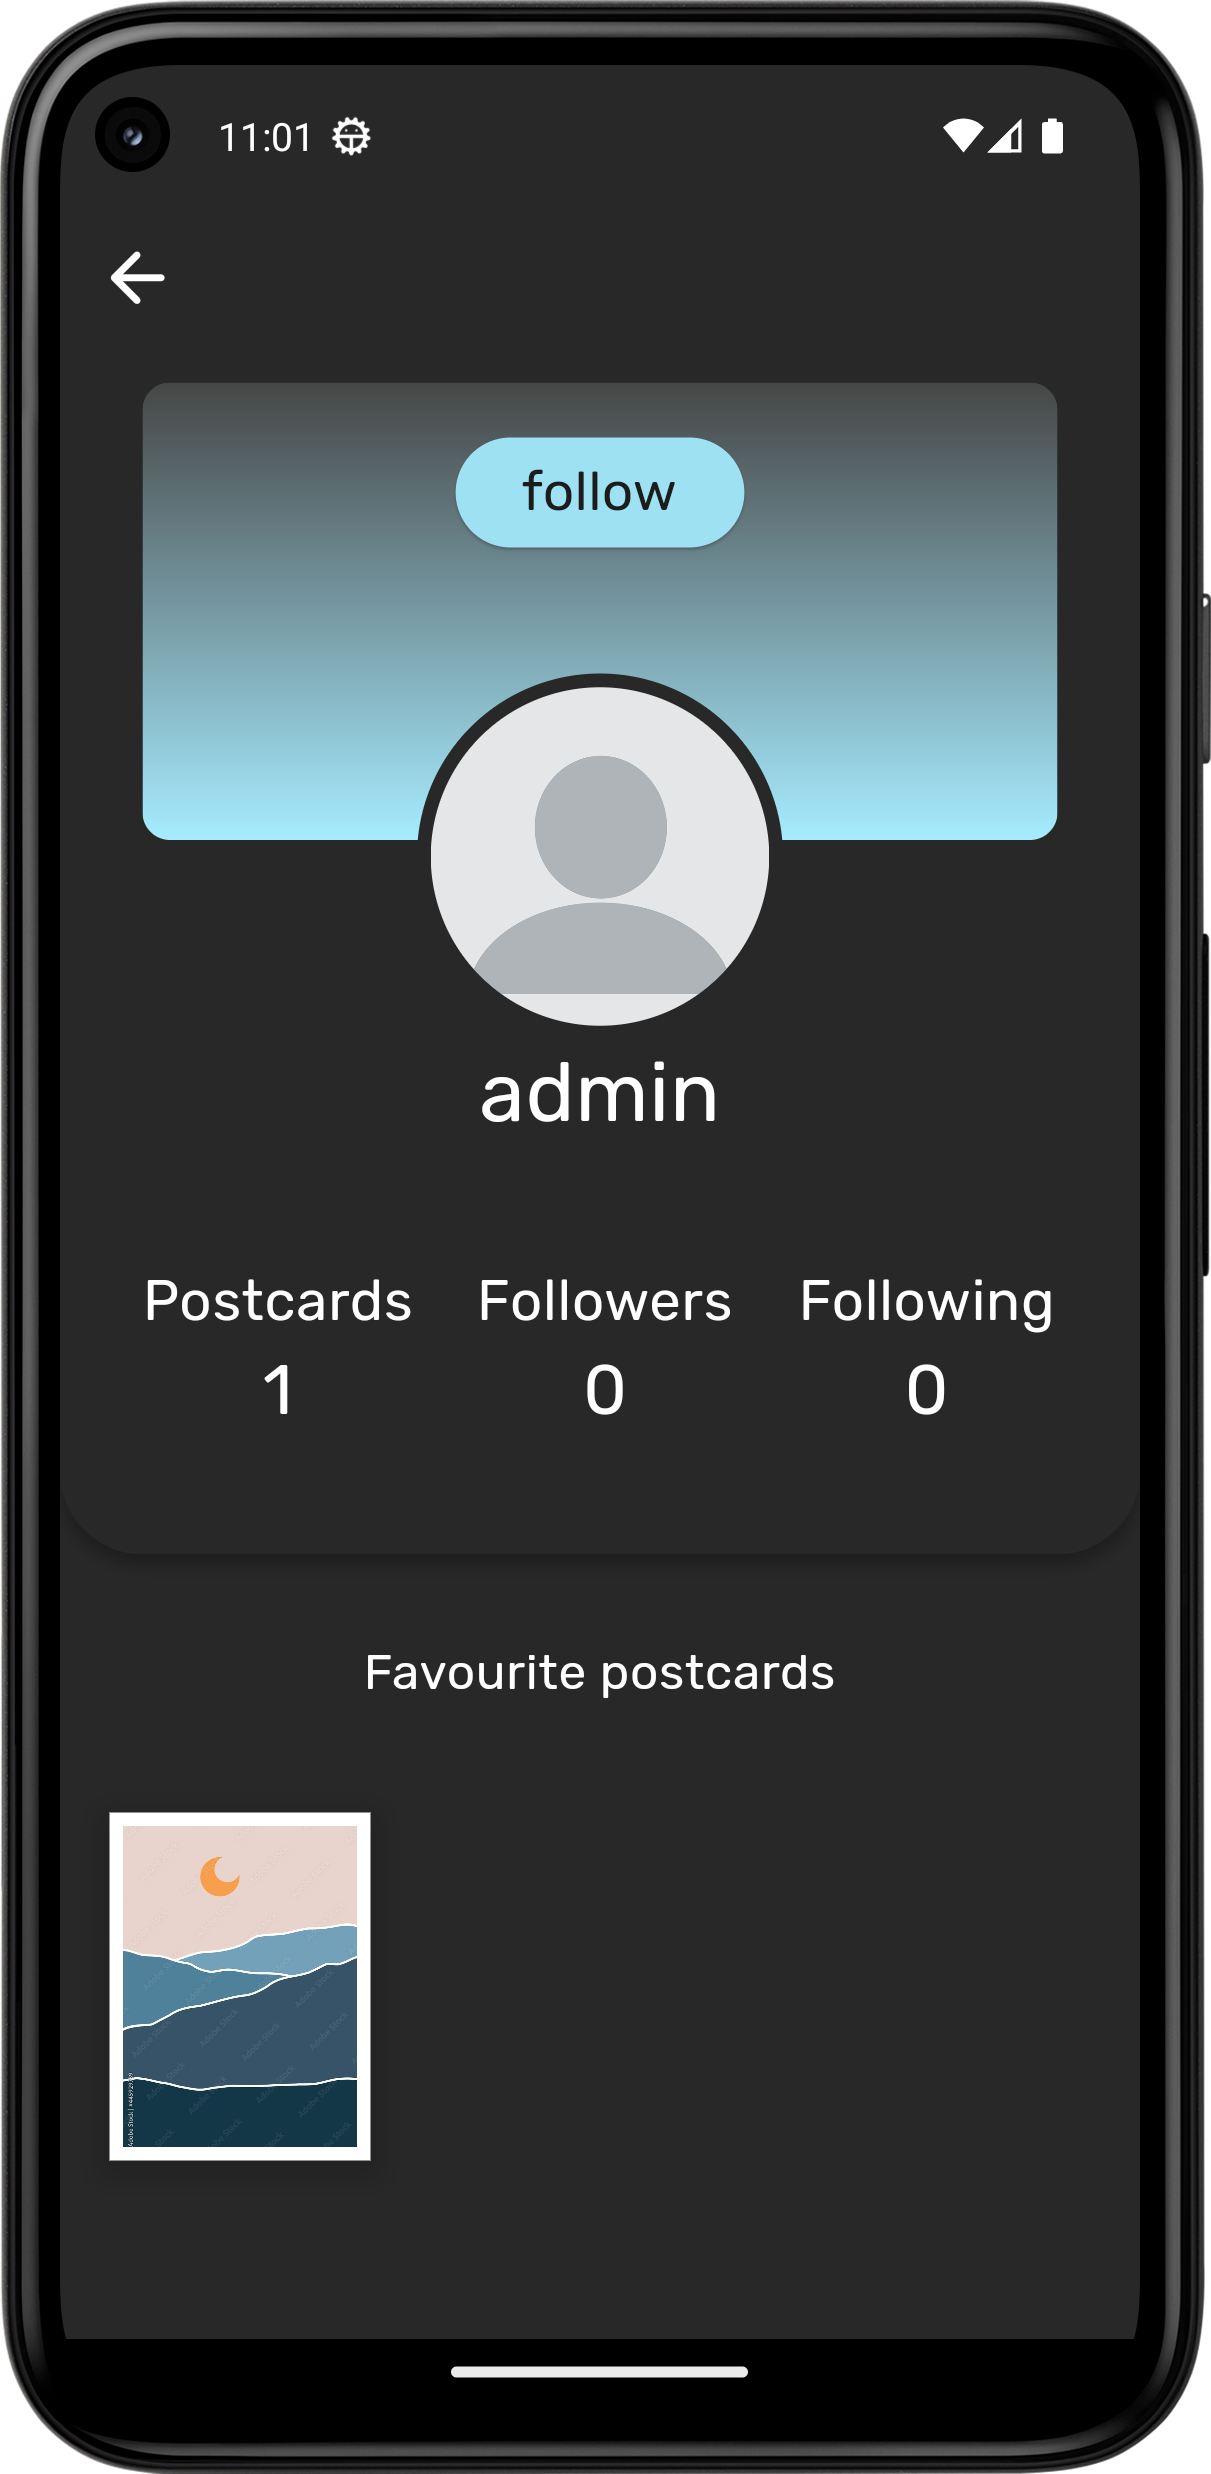
\includegraphics[width=0.5\textwidth]{mobile_ss/friend.png}
    \caption{Strona użytkownika}
\end{figure}

\subsection{Wysyłanie pocztówek}
Aby wysłać pocztówkę należy udać się na stronę z pocztówkami, tam po wybraniu odpowiedniej pocztówki na podglądzie wciskamy ``Send'' co przekieruje nas na podstronę do wysyłania pocztówek. Tam, możemy dodać tytuł oraz opis do pocztówki a następnie wybrać użytkownika do którego chcemy daną pocztówkę wysłać. 

\begin{figure}[H]
    \centering
    \includegraphics[width=0.5\textwidth]{mobile_ss/wysyłanie.png}
    \caption{Strona do wysyłania pocztówek}
\end{figure}

% ==========================================================================================
% ==========================================================================================
% ===================== BACKEND  ==========================================================================================

\chapter{Aplikacja serwerowa}
\section{Technologia}
Podczas wyboru technologii do realizacji aplikacji backendowej, kierowaliśmy się najnowszymi oraz najszybszymi rozwiązaniami. Docelowa platforma powinna być stale utrzymywana, dzięki czemu aplikacja mogłaby być z łatwością rozwijana w przyszłości. Popularne platformy cieszą się dużym zaangażowaniem społeczności, co umożliwia łatwiejsze rozwiązywanie napotkanych problemów. Ponadto możemy spojrzeć na gotowe rozwiązania, z których możemy czerpać dobre praktyki architektoniczne oraz rozwiązania. Wybór padł na technologie Microsoft, czyli język C\# oraz framework .NET 7.  

\subsection{Język C\#}
Język C\# jest silnie typowany oraz obiektowy, stworzony oraz rozwijany przez firmę Microsoft. Jest on częścią frameworka .NET, który umożliwia tworzenie aplikacji desktopowych, mobilnych, webowych.  Język C\# historycznie wzorowany jest na języku Java, czerpał z niego np. składnie, sposób działania. Dzięki byciu młodszą technologią wprowadza oraz doskonali wiele nowych rozwiązań.  
Do najważniejszych cech języka C\# można zaliczyć m.in.: 
\begin{itemize}
    \item Obiektowość - cała logika oraz sposób działania oparty jest na klasach. Podstawową klasą jest klasa ‘Object’ znajdująca się w przestrzeni nazw ‘System’. Każda inna dostępna klasa dziedziczy po niej. Dzięki czemu każda klasa w C\# posiada takie metody jak np. Equals(Object), GetType(), ToString(), oraz parę innych. 
    \item Zarządzanie pamięcią - język C\# podobnie jak Java posiada mechanizm Garbage Collector, dzięki któremu program automatycznie usuwa obiekty, które są już nieużywane. Dzięki takiemu rozwiązaniu programista nie musi dbać o ręczne zarządzanie pamięcią, co pozwala uniknąć problemów z jej wyciekiem. 
    \item LINQ – kwerendy Language Integrated Query umożliwiają pracę na obiektach, listach obiektów. Podobnie jak w języku SQL możemy pisać zapytania zwracające odpowiednie dane.
    \item Asynchroniczność - C\# pozwala na wykonywanie kodu w sposób wielowątkowy. Zawiera mechanizmy pozwalające wykonywać kod w sposób asynchroniczny, co jest istotne w przypadku nowoszesnych aplikacji webowych.
\end{itemize}

\subsection{Platforma .NET}
Platforma .NET stworzona przez Microsoft jest przeznaczona do tworzenia aplikacji na różne platformy. Obsługuje ona wiele języków programowania takich jak: C\#, F\#, Visual Basic. Sposób działania jest następujący. Docelowy język, w naszym przypadku to C\#, jest kompilowany przez kompilator do języka Common Intermediate Language (CIL). Następnie przechodzi przez Common Language Runtime (CLR). CLR to środowisko uruchomieniowe, które podczas uruchamiania aplikacji kompiluje kod przez just-in-time compiler (JIT). W ostatnim kroku kod tłumaczony jest na język maszynowy. Proces ten schematycznie przedstawiony został na rysunku 6.1.

\begin{figure}[h]
    \centering
    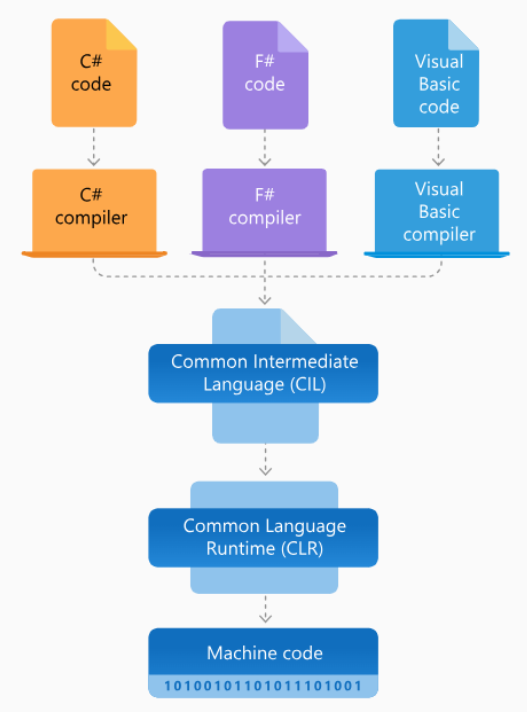
\includegraphics[width=0.5\textwidth]{compiler.png}
    \caption{Przepływ kompilowanego kodu \href{https://dotnet.microsoft.com/en-us/learn/dotnet/what-is-dotnet-framework}{https://dotnet.microsoft.com}.}
    \label{Kompilator}
\end{figure}

\subsection{Biblioteki}
W niniejszej sekcji zaprezentowano zastosowane w projekcie biblioteki wraz z ich krótkim opisem.
\subsubsection{Biblioteka główna}
    \begin{itemize}
        \item \textbf{ASP.NET Core 7.0} -- platforma programistyczna do tworzenia aplikacji.
    \end{itemize}
\subsubsection{Biblioteki pomocnicze}
    \begin{itemize}
        \item \textbf{Microsoft.EntityFrameworkCore} -- ORM (Object-Relational Mapping) biblioteka służąca do mapowania obiektami z bazy danych.
        \item \textbf{Microsoft.EntityFrameworkCore.Relational} -- dostarcza funkcjonalności, które usprawniają tworzenie relacji bazy danych.
        \item \textbf{Microsoft.EntityFrameworkCore.Design} -- zawiera logikę design-time. Są to narzędzia do projektowania baz danych oraz projektowania modelu danych.
        \item \textbf{Microsoft.EntityFrameworkCore.SqlServer} -- integracja frameworku z silnikiem bazy danych opartych na SQL Server.
        \item \textbf{Microsoft.EntityFrameworkCore.Tools} -- narzędzie do tworzenia migracji.
        \item \textbf{Microsoft.AspNetCore.Authentication.JwtBearer} -- implementacja funkcji dostarczających obsługę uwierzytelniania z wykorzystaniem tokenów JWT (JSON Web Token).
        \item \textbf{Swashbuckle.AspNetCore} -- dostęp do narzędzia Swagger, umożliwiającego generowanie dokumentacji na podstawie dostępnych w aplikacji endpointów.
        \item \textbf{Swashbuckle.AspNetCore.Annotations} -- wsparcie dla Swaggera, w postaci adnotacji.
        \item \textbf{AutoMapper} -– biblioteka służąca do mapowania obiektów znajdujących się pomiędzy różnymi warstwami.
        \item \textbf{AutoMapper.Extensions.Microsoft.DependencyInjection} -- rozszerzenie funkcji Automappera, o wstrzykiwanie zależności.
        \item \textbf{Microsoft.AspNetCore.Http} -- obsługa żądań HTTP.
        \item \textbf{Microsoft.Extensions.DependencyInjection.Abstractions} -- interfejsy dla systemu wstrzykiwania zależności.
        \item \textbf{Microsoft.Extensions.Identity.Core} -- biblioteka umożliwia dodawanie funkcji logowania do aplikacji.
        \item \textbf{Microsoft.NET.Test.Sdk}  -- narzędzia do tworzenia testów jednostkowych.
        \item \textbf{Moq} -- wykorzystanie w testach jednostkowych atrap pewnych funkcjonalności, w celu izolowania faktycznych implementacji od testów.
        \item \textbf{Xunit} -- framework do testów jednostkowych.
        \item \textbf{Unit.runner.visualstudio} -- program służący do uruchamiania testów jednostkowych.
    \end{itemize}

\section{Architektura}
W projekcie zastosowaliśmy architekturę Onion Architecture (Cebulowa Architektura). Wymusza ona na nas konkretne podejście do tworzenia oprogramowania. Dzięki ścisłym regułom oraz zasadom, tworzona aplikacja zawiera uporządkowany kod, podzielony na mniejsze projekty a dalej klasy. Aplikacja składa się z warstw pomiędzy, którymi występują odpowiednie zależności. Stąd pochodzi nazwa Onion Architecture.

\subsection{Onion Architecture}
\begin{itemize}
    \item \textbf{Warstwa Domain} -- nie posiada żadnej zależności, znajduje się w samym centrum warstw. Warstwa ta tworzy modele obiektów użytych później w bazie danych. Każdy z Modeli konfigurujemy, ustawiamy typ danych, jego właściwości. Jest również odpowiedzialna za logikę biznesową. 
    \item \textbf{Warstwa Application} -- posiada zależność do warstwy Domain. Warstwa ta posiada implementacje serwisów, czerpie dane z wartwy wewnętrznej, czyli Domain, a następnie przetwarza odpowiednio dane i przekazuje do warstwy zewnętrznej, czyli Infrastructure. 
    \item \textbf{Warstwa Infrastructure} -- posiada zależność do warstwy Application. Warstwa odpowiada za komunikację z bazą danych, wymienia się danymi z warstwą Application. 
    \item \textbf{Warstwa WebAPI} -- posiada zależność do warstwy Application oraz Infrastructure. Jej głównym celem jest obsługa zdarzeń z użytkownikiem oraz przekazywanie żądanych danych. Dane te są obsługiwane poprzez wykorzystanie protokołu HTTP. 
    \item \textbf{Warstwa Tests} -- posiada zależność do warstwy Application, dzięki czemu posiadamy możliwość wywoływania funkcjonalności z aplikacji. 
\end{itemize}

W celu dobrej komunikacji między poszczególnymi warstwami wykorzystujemy mechanizm Dependency Injection. Dependency Injection, inaczej wstrzykiwanie zależności pozwala na odpowiednie udostępnianie oraz zarządzanie zależnościami jakie występują pomiędzy warstwami w solucji. 

\subsection{Struktura plików}
Struktura plików w projekcie jest ściśle związana z zastosowaną architekturą Onion Architecture.
Cała solucja podzielona jest na parę projektów. Każdy z nich pełni odpowiednią rolę w swojej warstwie.  

\begin{enumerate}
    \item \textbf{WebAPI} \begin{itemize}
        \item \textbf{/Controllers} -- posiada implementacje wszystkich kontrolerów.
        \item \textbf{/Installers} -- znajdują się w nim wszystkie potrzebne instalacje zależności takie jak Cors, Baza danych, Cache, Uwierzytelnianie, MVC, Swagger. Każda zależność przydzielona jest do konkretnej klasy, która implementuje interfejs IInstaller. Podczas uruchomienia aplikacji wszystkie zależności, które implementują interfejs IInstaller, są odpowiednio wcześniej uruchomione przed startem web API. 
        \item \textbf{/Properties} -- zawiera plik, który definiuje właściwości uruchamiania aplikacji, takie jak adres Url, port, środowisko Swagger.
        \item \textbf{Program.cs} -- główny plik uruchomieniowy aplikacji serwerowej.
        \item \textbf{WebAPI.csproj} -- zawiera listę zewnętrznych bibliotek, zależności pomiędzy projektami oraz ustawienia projektu.
        \item \textbf{Appsettings.json} -- plik konfiguracji aplikacji.
        \item \textbf{Appsettings.development.json} -- plik konfiguracji aplikacji dla środowiska deweloperskiego.
    \end{itemize}

    \item \textbf{Application} \begin{itemize}
        \item \textbf{/Constants} -- stałe wartości, użyte w aplikacji.
        \item \textbf{/Dto} -- modele Data Transfer Object (DTO) - obiekty które zawierają konkretne pola, które chcemy przekazać dalej.
        \item \textbf{/Exceptions} -- spersonalizowane wyjątki.
        \item \textbf{/Helpers} -- pomocnicze funkcje.
        \item \textbf{/Interfaces} -- interfejsy do serwisów.
        \item \textbf{/Mappings} -- podzielony jest na konfiguracje Automappera wraz z obiektami zmapowanymi, oraz na folder /Manual, który zawiera manualnie zmapowane obiekty.
        \item \textbf{/Requests} -- obiekty dla żądania.
        \item \textbf{/Response} -- obiekty jako odpowiedź z endpointu.
        \item \textbf{/Services} -- implementacje serwisów.
        \item \textbf{/Validators} -- walidacja wybranych funkcjonalności z serwisu.
        \item \textbf{Application.csproj} -- zawiera listę zewnętrznych bibliotek, zależności pomiędzy projektami oraz ustawienia projektu.
        \item \textbf{DependencyInjection.cs} -- dodaje usługi o określonym typie w serviceType oraz wstrzykuje zależności.
    \end{itemize}

    \item \textbf{Domain} \begin{itemize}
        \item \textbf{/Configurations } -- konfiguracja dla obiektów bazy danych, taka jak: wymagane pola, typy danych.
        \item \textbf{/Entities} -- modele, które są odzwierciedleniem bazy danych.
        \item \textbf{/Enums} -- obiekty typu Enum.
        \item \textbf{/Interfaces} -- interfejsy dla repozytorium.
        \item \textbf{/Models} -- obiekty odpowiedzialne za przekazanie danych z filtrowania oraz paginacji z warstwy Domain do warstwy Infrastructure.
        \item \textbf{Domain.csproj} -- zawiera listę zewnętrznych bibliotek, zależności pomiędzy projektami oraz ustawienia projektu.
    \end{itemize}

    \item \textbf{Infrastructure} \begin{itemize}
        \item \textbf{/Data} -- konfiguruje dostęp do bazdy danych, implementuje ustawienia uwierzytelniania, zawiera Data Seeder, który wprowadza dane testowe do bazy danych.
        \item \textbf{/Migrations} -- lista plików migracyjnych.
        \item \textbf{/Repositories} -- lista repozytoriów aplikacji, wraz z generycznym repozytorium ‘Repository.cs’, po którym dziedziczy każde pozostałe repozytorium. Generyczne repozytorium posiada zaimplementowane podstawowe operacje CRUD.
        \item \textbf{DependencyInjection.cs} -- dodaje usługi o określonym typie w serviceType oraz wstrzykuje zależności.
        \item \textbf{Infrastructure.csproj} -- zawiera listę zewnętrznych bibliotek, zależności pomiędzy projektami oraz ustawienia projektu.
    \end{itemize}

    \item \textbf{Tests} \begin{itemize}
        \item \textbf{/Usings.cs} -- zawiera importy używanych zasobów.
        \item \textbf{Tests.csproj} -- zawiera listę zewnętrznych bibliotek, zależności pomiędzy projektami oraz ustawienia projektu.
        \item \textbf{*Tests.cs} -- są to konkretne implementacje testów jednostkowych, odpowiednie dla każdego repozytorium.
    \end{itemize}
\end{enumerate}

\subsection{Silnik bazy danych}
MSSQL, czyli kolejne rozwiązanie firmy Microsoft. Jest to system zarządzania relacyjną bazą danych. Szczególnie popularny i łączony z innymi rozwiązaniami Microsoftu, często łączony z aplikacjami .NETowymi. MSSQL jak każda relacyjna baza danych przechowuje informacje w tabelach, która składa się z wierszy oraz kolumn. Silnik pozwala nam na dowolną manipulacją danymi. Jest to rozwiązanie bezpieczne, umożliwia szyfrowanie danych. W połączeniu z systemem operacyjnym Windows mamy możliwość uwierzytelniania poprzez zintegrowany system. Największą zaletą, w porównaniu z konkurencyjnymi rozwiązaniami bazodanowymi, jest udostępnienie języka T-SQL na potrzeby MSSQL.

T-SQL, od transakcyjny SQL, to rozszerzenie języka SQL o znane z języków programowania mechanizmy takie jak: pętle, instrukcje warunkowe, zmienne. Dzięki temu rozszerzeniu tworzenie procedur oraz wyzwalaczy (ang. trigger) daje o wiele większe możliwości. Rozszerzenie pozwala przerzucić część funkcjonalności aplikacji backendowej na silnik bazy danych. Przydatne podczas implementacji funkcjonalności opartych na zmiany rekordów w bazie. Tworzenie wyzwalaczy, czyli funkcji wywołujących się automatycznie na bazie po spełnieniu konkretnego warunku, pozwala na uniknięcie niektórych błędów.

Do obsługi oraz podglądu bazy danych wykorzystane zostało narzędzie SQL Server Management Studio. Jest to zintegrowane środowisko zawierające wiele przydatnych funkcjonalności. 

\subsection{Modele}
Na poniższym rysunku 6.2 przedstawiony został schemat bazy danych wraz z relacjami. Do poprawnego działania aplikacji backendowej wymagana jest dobrze zaprojektowana i zaimplementowana baza danych. To ona przechowuje wszystkie informacje o użytkownikach, pocztówkach, posiadanych danych i całej reszcie. Na zaprezentowanym rysunku widoczne są wszystkie dostępne relacje. Przykładem relacji wiele do wielu może być połączenie tabeli User z tabelą Postcards poprzez tabelę pośredniczącą, czyli UserPostcards. Przykładem relacji jeden do jednego jest User z UserDetails. Relacja jeden do wielu zaprezentowana jest w PostcardData oraz Postcard. Znaczy to tyle, iż jeden rekord z tabeli PostcardData może występować w wielu rekordach w tabeli Postcard.

Najważniejszymi składowymi bazy danych są: User oraz Postcards. Jest to trzon naszej bazy, od których rozgałęziają się pozostałe relacje. Tabela User przechowuje podstawowe informacje o użytkowniku. Ma bezpośrednią relację jeden do jednego do UserStats, czyli statystyk użytkownika, UserDetails, czyli informacji szczegółowych, Address, czyli adresu użytkownika. Ponadto tabela User posiada relację wiele to wielu z tabelą UserFriends, ponieważ relacja ta odpowiada za posiadanie listy osób obserwujących oraz obserwowanych.

Tabela Postcards zbiera dane, które w połączeniu z tabelami: UserPostcards, FavouritePostcards, PostcardsCollection, PostcardData tworzą wspólną całość. Odpowiedzialna jest ona za zbieranie danych o posiadanych przez użytkownika pocztówkach - ich dostępności, pocztówkach ulubionych, odebranych i wysłanych.

Tabela \_\_EFMigrationsHistory zawiera historię o wykonanych migracjach przy użyciu biblioteki EntityFramework. 

\begin{figure}[H]
    \centering
    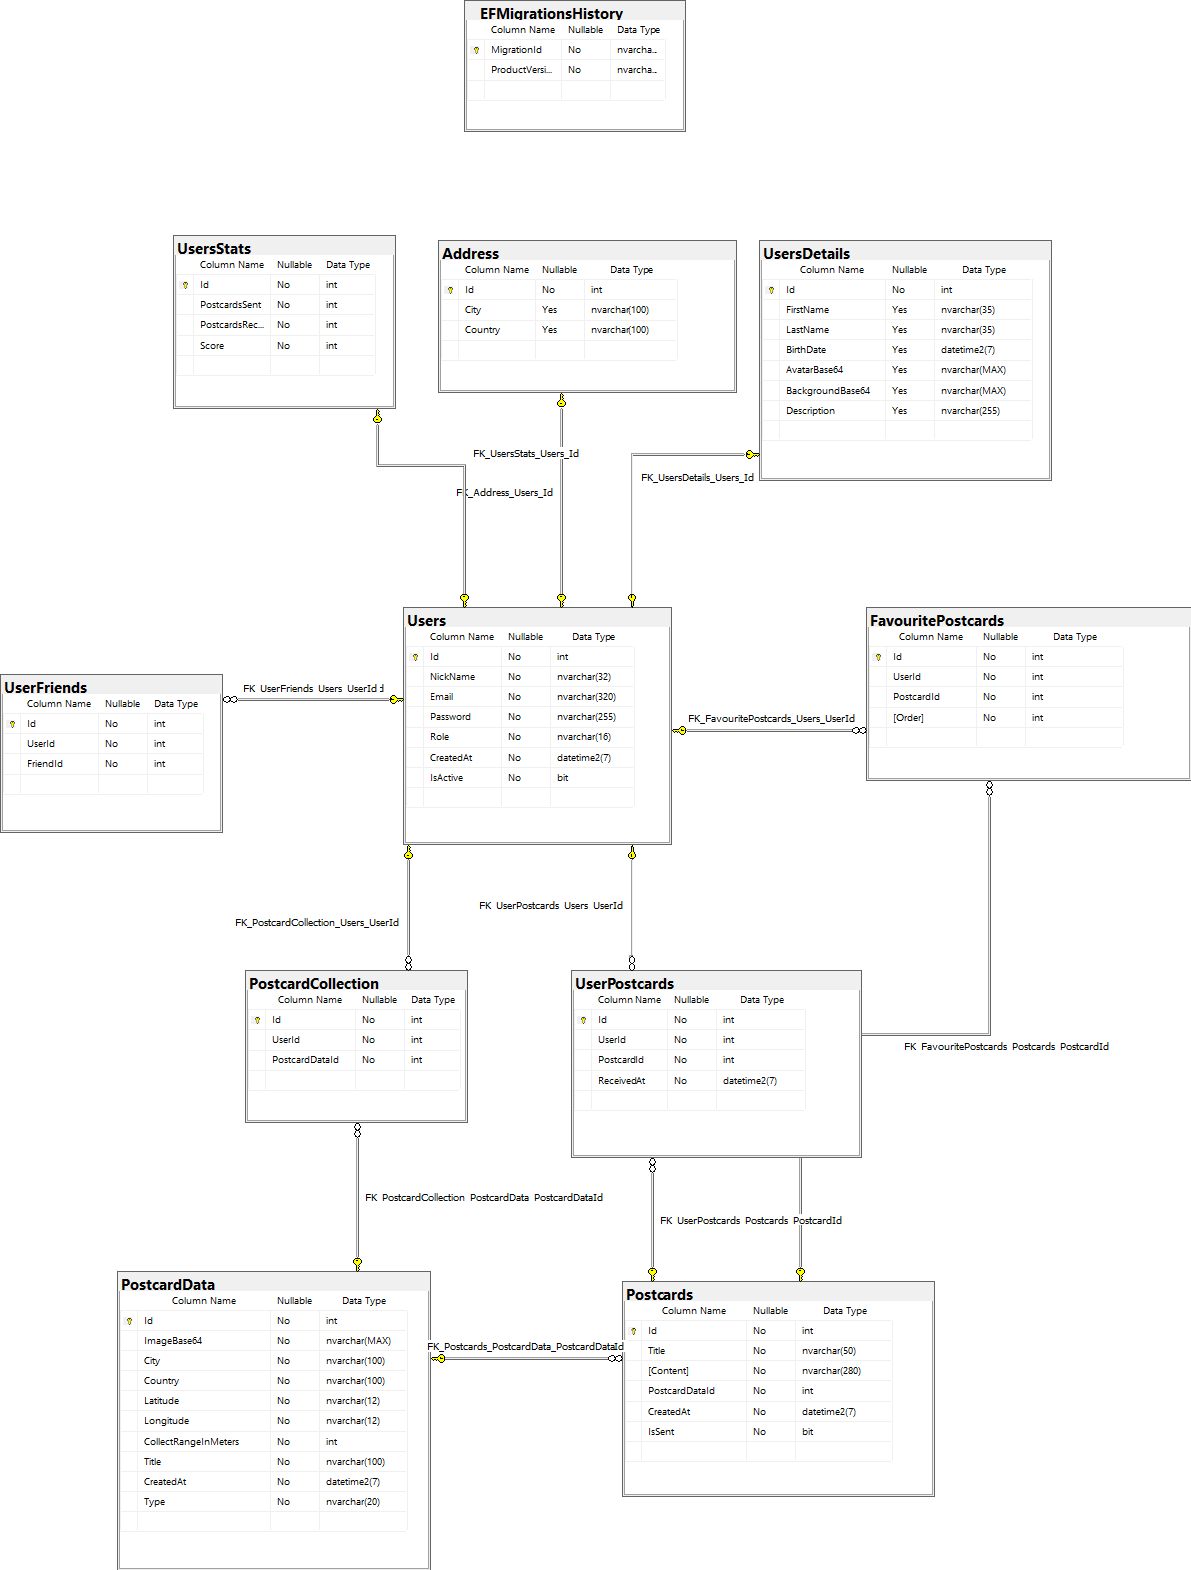
\includegraphics[width=1\textwidth]{diagram1.png}
    \caption{Diagram UML}
    \label{Kompilator}
\end{figure}

\section{Specyfikacja wewnętrzna}
Głównym plikiem uruchomieniowym aplikacji backendowej jest plik WebAPI/Program.cs. To właśnie w tym pliku definiujemy m.in. DataSeeder, Swaggera, użycie kontrolerów, mechanizmu uwierzytelniania oraz instalacji. Wykorzystując klasę WebApplicationBuilder tworzymy builder na podstawie, którego budowana jest aplikacja serwerowa. W celu usprawnienia budowania oraz tworzenia projektu zaimplementowaliśmy abstrakcyjny poziom instalacji zależności wraz z metodą instalującą InstallServicesInAssembly(). Abstrakcja ta polega na implementacji metody InstallService() w interfejsie IInstaller. W ten sposób zaimplementowane zostały instalacje metod potrzebnych dla: Cors, Swaggera, Cache, Authentication, MVC, Db. Zastosowanie tego rozwiązania pozwala utrzymać porządek w kodzie, zwłaszcza w tak kluczowym segmencie projektu. 

Definicje REST API warto rozpocząć od zdefiniowania czym jest samo API.  
API (Application Programming Interface), czyli interfejs programistyczny aplikacji jest opisem zasada, w jaki programy komunikują się między sobą. API możemy wyobrazić sobie jako most łączący dwa brzegi, przez który poruszają się samochody, czyli w tym przypadku nasze dane. Gdyby ten most nie istniał to komunikacja lądowa pomiędzy dwoma brzegami byłaby niemożliwa. Tak samo jest z API, które jest kluczowe do działania programu.  

REST (Representational State Transfer) API – styl architektoniczny, który opisuje w jaki sposób tworzony ma być rozproszony system. REST API zawiera w sobie sześć reguł projektowania: 
\begin{enumerate}
    \item \textbf{Jednolity interfejs} -- zapytania spełniają reguły formatowania API.
    \item \textbf{Rozdzielenie klient-serwer} -- klient oraz serwer to osobne aplikacje. Klient posiada informację o nazwie zasobu i w razie potrzeby pobiera ją z serwera. Natomiast serwer nie może ingerować w klienta. 
    \item \textbf{Bezstanowość} -- serwer nie musi przechowywać informacji o żądaniu.
    \item \textbf{Buforowość} -- mechanizm, który wymusza implementację cachu. Jeżeli dany zasób jest w krótkim czasie wywoływany kilkukrotnie to powinien być on zapisany w pamięci podręcznej. 
    \item \textbf{Warstwowa architektura systemu} -- końcowy klient nie musi posiadać wiedzy czy zasoby, o które prosi znajdują się na bezpośrednio pytanym serwerze, czy też na innym. Serwer może pełnić funkcję pośrednika pomiędzy zasobami dostępnymi w bazie danych a w bazach danych zewnętrznych dostawców. 
    \item \textbf{Kod na żądanie} -- klient może żądać wykonania kodu.
\end{enumerate}

Protokołem komunikacyjnym, który pomaga spełnić wymagania REST API jest HTTP. Protokół posiada metody, które umożliwiają pozyskanie jak i przesyłanie informacji. Metoda GET służy do pobierania zasobów, zwyczajowo nie zawiera elementu body. Metoda POST tworzy nowe zasoby, Metoda PUT może być wykorzystana do zaktualizowania zawartości. Metoda DELETE służy do usuwania zasobów.  

Kody odpowiedzi HTTP możemy podzielić na pięć kategorii: 
\begin{enumerate}
    \item \textbf{Grupa informacyjna}. Przedział: 100 – 199.
    \item \textbf{Grupa potwierdzenia sukcesu}. Przedział: 200 – 299.
    \item \textbf{Grupa przekierowania}. Przedział: 300 – 399.
    \item \textbf{Grupa błędu po stronie klienta}. Przedział: 400 – 499.
    \item \textbf{Grupa błędu po stronie serwera}. Przedział: 500 – 599.
\end{enumerate}

\subsection{Kontroler}
Aplikacja zawiera kontrolery w projekcie WebAPI. Każdej tabeli w bazie danych odpowiada jeden kontroler. Kontroler to punkt dostępu dla klienta, zawiera on endpointy wraz z różnymi metodami CRUD. Odpowiedzialny za wymianę danych z użytkownikiem końcowym. To on dzięki użyciu protokołu HTTPS oraz zasad RESTAPI dostarcza klientowi zasoby. W skład kontrolera wchodzą metody CRUD, czyli metody odpowiedzialne za tworzenie, czytanie, aktualizacje oraz usuwanie danych. Dostęp do każdego endpointu może być dodatkowo ograniczony poprzez uwierzytelnianie i/lub autoryzację. Endpointy zawierają informację o ścieżce dostępu. Po otrzymaniu żądania kontroler deleguje dalsze działanie do serwisów aplikacji, które to odpowiadają za realizację logiki aplikacji oraz zwrócenie danych do kontrolera. 

\subsection{Serwis}
Serwis odpowiada ze przetworzenie danych otrzymanych przez kontroler, a następnie zwracanie rezultatu. Jeśli jest taka potrzeba serwis może komunikować się z innymi serwisami lub zewnętrznymi usługami. W razie potrzeby działania na bazie danych serwis wykorzystuje metody napisane w repozytoriach.  

\subsection{Repozytorium}
Klasy odpowiedzialne za bezpośrednią komunikację serwera z bazą danych. To za jego pomocą pobieramy oraz zmieniamy dane w bazie. Dostęp do repozytorium powinny mieć jedynie serwisy, przy założeniu ze korzystamy z architektury Onion Architecture oraz, że chcemy odpowiednio zabezpieczyć warstwy. Repozytoria wykonują podstawowe operacje CRUD lub bardziej złożone zapytania. Elementarne operacje takie jak tworzenie nowego rekordu, jego zmiana, usunięcie lub pobranie go możemy wyabstrahować do formy generycznych metod. 

\subsection{Generyczne repozytorium}
Generyczne repozytorium zawiera implementacje najprostszych metod CRUD. Umożliwia to w bardzo szybki sposób na implementację podstawowych funkcjonalności w aplikacji. Dodatkowo pozbywamy się zbędnych powtórzeń kodu, ponieważ operacje CRUD w większości przypadków są powtarzalne. W naszej aplikacji stworzyliśmy podstawową klasę Repository, od której to pozostałe repozytoria dziedziczą. Repository przyjmuje jako argument generyczny model dla tabeli, na której chcemy wykonywać operacje. Przez takie rozwiązanie generyczne metody mogą operować jedynie na jednej tabeli w tym samym czasie. W razie utworzenia bardziej zaawansowanych operacji poza istniejącą implementacją możemy wdrożyć dodatkowe metody. Przykładem mogą być operacje na bazie na wielu tabelach. 

\subsection{Migracje}
Entityframework Core dostarcza narzędzi do tworzenia migracji bazy danych.  

W projekcie wykorzystaliśmy podejście Model-First. Polega ono na stworzeniu encji oraz relacji, a następnie na ich podstawie EFCore generuje zapytania do bazy danych. Podejście takie stosowane jest zazwyczaj w przypadku, kiedy nie posiadamy jeszcze istniejącej bazy danych. Podejściem odwrotnym jest podejście Database-First. W tym przypadku to modele, relacje oraz mapowania są tworzone na podstawie istniejącej bazy danych. 

Aby utworzyć migrację wykorzystujemy polecenie Add-Migration <Nazwa>. Dzięki niemu tworzone są dwa pliki. W skład ich nazw wchodzi rok, miesiąc, dzień, godzina wykonania migracji oraz podana przez nas nazwa <Nazwa>. Dzięki zastosowanej składni rozwiązuje się kilka problemów. Po pierwsze taka nazwa jest jednoznacznie zidentyfikowana z konkretnymi zmianami. Po drugie dzięki formatowi daty, aplikacja wie w jakiej kolejności wywołać migrację, dzięki czemu unikniemy problemu z niepoprawną kolejnością ich wywoływania. 
Zawartość pliku migracji.cs to klasa zawierająca metody: Up() oraz Down(). Metoda Up() tworzy tabele, określa kolumny oraz relacje. Definiuje klucze główne oraz obce. Metoda Down() definiuje operację, które należy wykonać, aby cofnąć zmiany z metody Up(). Przydatne w razie pomyłki oraz potrzeby cofnięcia zmian.
Natomiast plik migracja.Designer.cs definiuje encje, które odpowiadają modelom w kodzie.
W celu wprowadzenia zmian z migracji do bazy danych należy skorzystać z polecenia Update-Database. Na rysunku 6.3 przedstawiono przykładowy plik migracyjny, zawierający informację o tworzonej nowej tabeli.
\begin{figure}[H]
    \begin{lstlisting}
using Microsoft.EntityFrameworkCore.Migrations;

#nullable disable

namespace Infrastructure.Migrations;

/// <inheritdoc />
public partial class InitializeDatabase : Migration
{
    /// <inheritdoc />
    protected override void Up(MigrationBuilder migrationBuilder)
    {
        migrationBuilder.CreateTable(
            name: "PostcardsImages",
            columns: table => new
            {
                Id = table.Column<int>(type: "int", nullable: false)
                    .Annotation("SqlServer:Identity", "1, 1"),
                ImageBase64 = table.Column<string>(type: "nvarchar(max)", nullable: false)
            },
            constraints: table =>
            {
                table.PrimaryKey("PK_PostcardsImages", x => x.Id);
            });
...
    migrationBuilder.CreateIndex(
                name: "IX_Postcards_ImageId",
                table: "Postcards",
                column: "ImageId");
        }

        /// <inheritdoc />
        protected override void Down(MigrationBuilder migrationBuilder)
        {
            migrationBuilder.DropTable(
                name: "PostcardsImages");
        }
    }
}
    \end{lstlisting}
\caption{Automatycznie wygenerowany plik migracyjny}
\label{fig:pseudokod:listings}
\end{figure}

\subsection{Interfejs}
Interfejs w C\# podobnie jak w innych obiektowych językach programowania to abstrakcyjny typ posiadający jednie deklaracje. Nie możemy stworzyć na jej podstawie obiektu, natomiast każda klasa lub struktura może zaimplementować dowolnie wiele interfejsów. Warunkiem do poprawnego użycia interfejsu jest konieczność implementacji wszystkich zdefiniowanych w interfejsie metod. Interfejsów używamy w celu osiągnięcia pewnego poziomu abstrakcji. Przykładem użycia jest interfejs IRepository, po którym to dziedziczy każde z repozytoriów. Ponadto każde repozytorium oraz serwis posiadają swój indywidualny interfejs. Stosowane jest to w celu poprawnej implementacji architektury Onion Architecture. Dla przykładu implementacja repozytoriów znajduje się w projekcie Infrastructure, natomiast ich interfejsy znajdują się w warstwie Domain. Jest tak, ponieważ oddzielamy w ten sposób logikę biznesową od domeny. Ułatwia to późniejsze testowanie aplikacji. 

\subsection{Wstrzykiwanie zależności}
Dependency injection – wstrzykiwanie zależności stosowane jest do zarządzania zależnościami w ramach całej solucji. W ramach konkretnych projektów może być potrzeba na zarejestrowanie usługi i/lub jej użycie. W ramach rejestracji usług interfejs IServiceCollection dostarcza metody. Trzy główne oraz najczęściej stosowane to: AddScoped, AddTransient i AddSingleton. 
\textbf{AddScoped} -- usługa tworzona jest raz podczas pojedynczego żądania HTTP, przy każdym zapytaniu otrzymujemy nowy obiekt 
\textbf{AddTransient} -- dla każdego żądania usługi zostaje tworzona nowa instancja 
\textbf{AddSingleton} -- to nic innego jak użycie wzorca projektowego Singleton. Pozwala stworzyć usługę tylko raz podczas trwania działania aplikacji. Używane jest podczas gdy dane które są w tej usłudze rejestrowane, są współdzielone w wielu miejscach. 


\subsection{Uwierzytelnianie i autoryzacja (JWT)}
We współczesnych implementacjach aplikacji ważne są pojęcia takie jak uwierzytelnianie oraz autoryzacja. Istotny jest poziom bezpieczeństwa użytkowników oraz ich danych. Często są to dane wrażliwe, które po dostaniu się w niepowołane ręce mogą wyrządzić wiele szkód użytkownikowi jak i wiele problemów organizacji oraz twórcą wadliwego oprogramowania. 

Uwierzytelnianie to proces, podczas którego potwierdzamy tożsamość użytkownika. Celem jest upewnienie się, że osoba, która wykonuje pewne żądanie może uzyskać zasób lub jego część. Uwierzytelniamy się w systemie np. poprzez podanie hasła, użycie karty dostępu lub poprzez skorzystanie z zewnętrznych serwisów. 

Autoryzacja to z kolei proces, który odpowiada na pytanie “Czy jesteś uprawniony to zrobić?”. Użytkownicy po zalogowaniu mają różne uprawnienia do zasobów. Związane jest to z różnymi rolami oraz uprawnieniami w aplikacji, organizacji. To za pomocą autoryzacji jesteśmy w stanie ograniczyć dostęp do zasobów. 

Na rysunku 6.4 przedstawiono w sposób schematyczny proces uwierzytelniania.
\begin{figure}[H]
    \centering
    \includegraphics[width=1\textwidth]{jwt.png}
    \caption{JWT przepływ uwierzytelniania}
    \label{JWT}
\end{figure}

\subsection{Proces uwierzytelniania} 
Proces uwierzytelniania zaczyna się od użytkownika oraz aplikacji klienckiej z wbudowanym formularzem logowania. Użytkownik po wpisaniu danych logowania wysyła prośbę o uwierzytelnienie na serwer. Ten natomiast sprawdza czy podane dane są zgodne ze stanem faktycznym w bazie danych. Następnie tworzy token, który zawiera informacje o użytkowniku oraz długości życia sesji. Przekazuje je do aplikacji klienta. Klient posiadając taki token ma możliwość z dalszego korzystania z aplikacji oraz dostępu do zablokowanych źródeł. Podczas każdego autoryzowanego zapytania klient wysyła w nagłówku otrzymany token, co pozwala serwerowi na dalszą autoryzację oraz uwierzytelnianie użytkownika. W przypadku niepoprawnego tokenu lub błędnych danych przekazanych na serwer, aplikacja klienta odmówi dostępu do niedostępnych danych. 

\subsection{Czym jest token JWT?} 
JWT (JSON Web Token) - token wydawany przez serwer. Jest to ciąg znaków kodowany do Base64. Jest on nie szyfrowany, oznacza to, że każdy jest w stanie odkodować jego zawartość. Co za tym, nie mogą znajdować się w nim dane wrażliwe, a jedynie informacje o nazwie użytkownika, jego id lub podobne. Każdy token ma określoną długość życia. W ramach każdego zapytania długość ta może być przedłużana przy pomocy RefreshTokena, aby zachować ciągłość działania aplikacji bez potrzeby ponownego logowania. 

RefreshToken to specjalny token, który zostaje użyty w przypadku, gdy nasz token dostępu utraci swoją ważność. RefreshToken ma dłuższy czas życia niż token dostępu. 

W skład tokenu wchodzi: nagłówek, payload, podpis tokena. Nagłówek to informacja o użytym algorytmie podpisywania tokena. Payload jest to lista wszystkich claimsów. Podpis tokena to suma kontrola. Claim to informacja o danych zalogowanego użytkownika. Przydatne podczas tworzenia tokenów JWT. Każdy token JWT może posiadać parę różnych Claimsów.  

\begin{figure}[H]
    \centering
    \includegraphics[width=1\textwidth]{jwtdecode.png}
    \caption{Przykładowe zdekowodanie tokenu JWT }
    \label{JWTDecode}
\end{figure}

\subsection{Data seeder} 
W celu ułatwienia procesu deweloperskiego na nasze wewnętrzne potrzeby stworzony został mechanizm wprowadzania danych. Jest to specjalny zestaw klas oraz metod, które wywoływane są jedynie na środowisku testowym. Metody te wprowadzają dane testowe do naszej bazy danych.  

Główną klasą, która zarządza danymi jest klasa DataSeeder. Posiada metodę Seed(), która jest wywoływana wraz z uruchomieniem programu. Sprawdza ona czy nasze połączenie z bazą testową jest prawidłowe oraz następnie dla każdej tabeli sprawdza czy posiada ona już jakieś testowe dane. Jeśli dana tabela nie posiada danych testowych to za pomocą odpowiadających im klas statycznych wprowadza dane testowe do tabeli. Dzięki temu rozwiązaniu dane testowe nie są dublowane przy każdym uruchomieniu aplikacji, a jedynie w momencie, gdy tabela jest pusta. Takie rozwiązanie bardzo ułatwia testowanie aplikacji oraz symulowanie rzeczywistego działania na danych. 

\subsection{Cachowanie} 
Podczas tworzenia aplikacji backendowej ważnym aspektem jest jego optymalizacja oraz szybkość działania. Jednym z mechanizmów pozwalającym zwiększyć wydajność aplikacji jest mechanizm cachowania, czyli przechowywania tymczasowych kopii. Cache obejmuje przechowywanie danych pozyskanych z bazy danych, plików które są dostępne z poziomu backendu. Stosowanie cachingu zwiększa wydajność poprzez ograniczenie ilości powtórnie wykonywanych operacji odczytu. Dla przykładu, jeżeli użytkownik odczyta jakieś dane, a w niedalekiej przyszłości zrobi to ponownie, to dzięki zastosowaniu mechanizmu cache ta druga operacja nie będzie musiała być ponownie obliczona przez serwer. Zostaną jedynie zwrócone dane które były zapisane w pamięci podręcznej podczas pierwszego zapytania. Minusem takiego zastosowania jest oczywiście zużycie pamięci, przez co należy używać tego mechanizmu z rozwagą i jedynie w kluczowych miejscach. Druga sprawa to taka, że jeżeli dane zostały zmienione pomiędzy zapytaniami a my mamy dostęp do przestarzałego cache, który może być wynikiem błędnej implementacji, to użytkownik otrzyma niezaktualizowane dane. I to właśnie na poprawną implementację powinniśmy zwrócić uwagę. Ponieważ podczas fazy deweloperskiej utrudnia to poprawne zlokalizowanie błędów, a podczas korzystania z wydanej aplikacji zwrócić może nieaktualne dane. 
W C\#, aby zrealizować mechanizm cachowania możemy skorzystać z przestrzeni nazw Microsoft.Extensions.Caching.Memory oraz interfejsu IMemoryCache. W standardowy sposób wstrzykujemy przez kontruktor obiekt IMemoryCache, a następnie za pomocą metody Set() możemy ustawić klucz oraz wartość danej kopii. Aby poprawnie stworzyć kopię tymczasową, potrzebujemy klucza, który jednoznacznie zidentyfikuje daną kopię, dane które chcemy zapamiętać, oraz opcjonalnie ustawienia. Do skorzystania z ustawień należy użyć klasy MemoryCacheEntryOptions. To w niej możemy zawrzec takie informacje jak np. czas przechowywania kopii w pamięci, jego priorytetu oraz rozmiar danych. Do tworzenia kluczy stworzona została statyczna klasa CacheKeyGenerator. Posiada przeciążoną metodę GetKey(), która to przyjmuje jako argumentu różne wartości, zależne od kontekstu aplikacji. 

Mechanizm cache zastosowaliśmy podczas pobierania danych pocztówek oraz użytkownika. Związane jest to z tym, że powyższe wartości bardzo rzadko ulegają zmianie. Dzięki temu serwer nie musi za każdym zapytaniem ponownie przetwarzać danych, co wpływa na szybkość z jaką otrzymujemy dane z serwera.

\subsection{Mapper} 
Mapowanie, czyli funkcja, która zamienia jeden obiekt do postaci innego obiektu. Stosowana jest w celu uniknięcia przypisywania każdego pola do nowego obiektu, pozwala to uniknąć powtórzeń w kodzie oraz usprawnić proces przekazywania danych. Częstym miejscem w kodzie, gdzie stosuje się mapowanie np. przekazywanie obiektu z zapytania użytkownika do następnej warstwy aplikacji. Na tym etapie otrzymujemy od użytkownika szczątkowe informacje o obiekcie, ale przy pomocy mappera tworzymy nowy obiekt, który zawiera brakujące pola. Ten nowy obiekt następnie może posłużyć do wykonania działań na bazie danych przy pomocy repozytoriów.

W kodzie zastosowaliśmy dwa podejścia do mappera. Pierwsze, z wykorzystaniem biblioteki AutoMapper, która to po uprzednim skonfigurowaniu pozwala w znaczący sposób zautomatyzować proces mapowania. Służą do tego wewnętrzne funkcje biblioteki. Każdy z obiektów DTO (Data Transfer Object), czyli obiektów transferów danych, posiada zaimplementowaną metodę Map. Ponadto posiadamy osobną klasę AutoMapperConfig, w której to znajduje się dalsza część mapowania obiektów.

Drugim podejściem jest mapowanie manualne przy pomocy ręcznie napisanych klas. Wszystkie nasze klasy mapera znajdują się w folderze /Application/Mapping/Manual. Są to klasy statyczne które jako argument przyjmują obiekt klasy wchodzącej, a zwracają obiekt klasy docelowej.

Różnica pomiędzy oboma podejściami jest taka, że w podejściu z wykorzystaniem AutoMappera, wiele zadań jest wykonanych automatycznie bez naszego udziału. Natomiast potrzebna jest wcześniejsza konfiguracja, która miejscami może być o wiele trudniejsza. W przypadku manualnych maperów mamy do czynienia z większą ilością kodu, jednak pisanie tych klas jest bardzo proste i mamy większą kontrolę nad procesem mapowania np. w przypadku debugowania kodu.

\subsection{Swagger}
Swagger to narzędzie, które pozwala w łatwy oraz przystępny sposób na korzystanie z naszego API. Dodatkowo pełni funkcję dokumentacji. Dane te można eksportować i użyć w Postmanie lub innych programach do testowania API. Każdy z endpointów możemy dowolnie testować. Można przekazywać dowolne dane, a dzięki wbudowanym mechanizmom istnieje możliwość wstrzyknięcia tokenu JWT, dzięki czemu nie mamy żadnych ograniczeń. W naszej aplikacji serwerowej, Swagger uruchamiany jest automatycznie podczas rozpoczęcia działania aplikacji. Jego sesja gaśnie wraz z zamknięciem okna przeglądarki lub wyłączenia backendu.

\section{Ważne funkcjonalności}
\subsection{Wzór Haversine}
W celu poprawnej implementacji systemu powiadomień oraz systemu odbierania pocztówek, należy obliczyć odległość ortodromiczną. Odległość ortodromiczna to najkrótsza droga pomiędzy dwoma punktami na powierzchni kuli. W tym celu posłuży wzór Haversine.

    \begin{equation}
    d = 2R \arcsin\left( \sqrt{\sin^2\left(\frac{{\text{{lat}}_2 - \text{{lat}}_1}}{2}\right) + \cos(\text{{lat}}_1) \cdot \cos(\text{{lat}}_2) \cdot \sin^2\left(\frac{{\text{{lon}}_2 - \text{{lon}}_1}}{2}\right)} \right),
    \end{equation}
    gdzie:
    \begin{align*}
    \text{{lat}}_1 & : \text{{szerokości geograficzna pocztówki}} \\
    \text{{lat}}_2 & : \text{{szerokości geograficzna użytkownika}} \\
    \text{{lon}}_1 & : \text{{długość geograficzna}} \\
    \text{{lon}}_2 & : \text{{długość geograficzna}} \\
    R & : \text{{promień ziemi}}
    \end{align*}

Powyższy wzór został wykorzystany w aplikacji serwerowej. Jest to jedna z najważniejszych funkcji w programie, ponieważ to ona mówi o tym czy użytkownik znajduje się w zasięgu odebrania pocztówki.
    
\subsection{Uwierzytelnianie}
Uwierzytelnianie jako kluczowy proces aplikacji, powinien być odpowiednio zabezpieczony oraz obsługiwany. Ważne jest, aby hasła były zapisywane w bazie danych w formie zahaszowanej, a następnie, aby proces logowania odpowiednio dostosowywał dane logowania pod zahaszowaną formę danych.

Metoda, która obsługuje rejestrację użytkownika zawiera wiele walidatorów. Na każdym etapie sprawdzamy czy podane dane do rejestracji są prawidłowe. Hasła muszą być takie same, nie mogą być za krótkie. Email musi być unikalny oraz posiadać poprawną składnie. Jeżeli warunki te zostaną spełnione to zostaje założone nowe konto użytkownika. Hasło zostaje zapisane w bazie danych w postaci zahaszowanej. Na rysunku 6.6 znajduje się implementacja metody rejestracji użytkownika. Jako argument funkcja przyjmuje obiekt DTO - RegisterUserDto. Następnie w kolejnych krokach dane te poddane są walidacji. Po jej poprawnym przejściu zostaje utworzony nowy użytkownik.

\begin{figure}[H]
    \begin{lstlisting}
public async Task<RegisterResponse> Register(RegisterUserDto registerUserDto)
{
    RegistrationResult result = RegistrationResult.Success;
    if (registerUserDto.Password != registerUserDto.ConfirmPassword)
    {
        result = RegistrationResult.PasswordsDoNotMatch;
    }
    if (registerUserDto.Password.Length < UserServiceConstants.MinPasswordLength)
    {
        result = RegistrationResult.WeakPassword;
    }
    if (!EmailRegex.IsValidEmail(registerUserDto.Email))
    {
        result = RegistrationResult.IncorrectEmail;
    }
    bool isEmailInUse = _userRepository.IsEmailInUse(registerUserDto.Email);
    if (isEmailInUse)
    {
        result = RegistrationResult.EmailAlreadyExists;
    }
    if (result != RegistrationResult.Success)
    {
        throw new Exception(result.ToString());
    }
    User newUser = _mapper.Map<User>(registerUserDto);
    string hashedPassword = _passwordHasher.HashPassword(newUser, registerUserDto.Password);
    newUser.Password = hashedPassword;
    newUser.Role = "USER";
    newUser.CreatedAt = DateTime.UtcNow;

    User user = await _userRepository.Insert(newUser);
    await _userStatsRepository.Insert(new UserStat() { Id = user.Id, PostcardsReceived = 0, PostcardsSent = 0, Score = 0 });
    await _addressRepository.Insert(new Address() { Id = user.Id });
    await _userDetailRepository.Insert(new UserDetail() { Id = user.Id });
    RegisterResponse registerResponse = _mapper.Map<RegisterResponse>(user);
    return registerResponse;
}
    \end{lstlisting}
\caption{Metoda rejestracji użytkownika}
\label{fig:pseudokod:listings}
\end{figure}

W celu poprawnego przetworzenia procesu logowania hasło musimy zweryfikować przy pomocy specjalnej funkcji VerifyHashedPassword, która to sprawdza czy zahaszowane hasło jest tym samym hasłem, które podaje użytkownik w formularzu logowania. 

Proces logowania został przedstawiony na rysunku 6.7. Przekazujemy obiekt LoginUserDto, który zawiera dane logowania.
\begin{figure}[H]
    \begin{lstlisting}
public Task<LoginResponse> Login(LoginUserDto loginUserDto)
{
    User storedUser = _userRepository.GetUserByEmail(loginUserDto.Email) ?? throw new Exception("User not found");
    PasswordVerificationResult passwordResult = _passwordHasher.VerifyHashedPassword(storedUser, storedUser.Password, loginUserDto.Password);
    if (passwordResult != PasswordVerificationResult.Success)
    {
        throw new Exception("Password is incorrect");
    }

    User userDataForClaims = _userRepository.GetUserByEmail(loginUserDto.Email);
    LoginResponse loginResponse = new LoginResponse() { Token = _userRepository.Login(userDataForClaims) };
    return Task.FromResult(loginResponse);
}
    \end{lstlisting}
\caption{Metoda rejestracji użytkownika}
\label{fig:pseudokod:listings}
\end{figure}

Po zakończeniu procesu logowania sukcesem, zwracany jest token JWT. Na dalszym etapie obsłuży on procesy związane z uwierzytelnianiem oraz autoryzacją. Jak możemy zauważyć tworzona jest lista Claimsów. Zawiera ona informację, które następnie będą dostępne z poziomu tokena JWT. Są to informacje o ID użytkownika, jego nicku, emailu oraz roli.

Na rysunku 6.8 przedstawiony został proces tworzenia tokenu JWT. Na początku definiujemy Claimsy, w kolejnych krokach długość życia tokenu.
\begin{figure}[H]
\begin{lstlisting}
public string Login(User user)
{
    List<Claim> claims = new List<Claim>()
    {
        new Claim(ClaimTypes.NameIdentifier, user.Id.ToString()),
        new Claim(ClaimTypes.Name, user.NickName),
        new Claim(ClaimTypes.Email, user.Email),
        new Claim(ClaimTypes.Role, user.Role),
    };

    SymmetricSecurityKey key = new SymmetricSecurityKey(Encoding.UTF8.GetBytes(_authenticationSettings.JwtKey));
    SigningCredentials credentials = new SigningCredentials(key, SecurityAlgorithms.HmacSha256);
    DateTime expires = DateTime.Now.AddDays(_authenticationSettings.JwtExpireDays);

    JwtSecurityToken token = new JwtSecurityToken(
        _authenticationSettings.JwtIssuer,
        _authenticationSettings.JwtIssuer,
        claims,
        expires: expires,
        signingCredentials: credentials
    );

    JwtSecurityTokenHandler tokenHandler = new JwtSecurityTokenHandler();
    return tokenHandler.WriteToken(token);
}
\end{lstlisting}
\caption{Metoda tworząca token JWT}
\label{fig:pseudokod:listings}
\end{figure}

\subsection{Przekazywanie pocztówki}
Przekazywanie pocztówki to proces, w którym użytkownik wybierając adresata oraz jedną ze swoich nowych pocztówek wysyła tę pocztówkę wraz z opisem. Opisem może być dowolna treść. Może to być pozdrowienie z wakacji, opisanie jakieś historii lub pewna forma komunikacji. W skład opisu wchodzi nagłówek pocztówki oraz treść właściwa. 

        \begin{figure}[H]
        \begin{lstlisting}
public async Task<UserPostcardDto> TransferPostcard(int newUserId, PostcardDto postcardDto)
{
    if (!await _userService.IsUserActive(newUserId))
    {
        throw new Exception("User is not active");
    }

    UserPostcard userPostcard = await _userPostcardRepository.GetUserPostcardByPostcardId(postcardDto.Id);
    if (!PostcardTransferValidator.IsPostcardValid(userPostcard, newUserId, _userContextService.GetUserId))
    {
        throw new Exception("Postcard is not valid");
    }

    PostcardDto postcard = await GetPostcardById(postcardDto.Id);
    UserStatDto sender = await _userStatsService.GetUserStatsById(_userContextService.GetUserId ?? userPostcard.UserId);
    UserStatDto receiver = await _userStatsService.GetUserStatsById(newUserId);

    if (postcard.IsSent)
    {
        throw new Exception("Postcard already received by user");
    }

    if (!PostcardTransferValidator.IsSenderAndReceiverValid(sender, receiver))
    {
        throw new Exception("User not found");
    }
...
        \end{lstlisting}
    \caption{Metoda tworząca token JWT 1/2}
    \label{fig:pseudokod:listings}
    \end{figure}

    \begin{figure}[H]
        \begin{lstlisting}
...
        
    sender.PostcardsSent++;
    sender.Score++;
    receiver.PostcardsReceived++;
    receiver.Score++;
    postcard.IsSent = true;
    postcard.Title = postcardDto.Title;
    postcard.Content = postcardDto.Content;

    await UpdatePostcard(postcard);
    await _userStatsService.UpdateUserStats(sender);
    await _userStatsService.UpdateUserStats(receiver);

    userPostcard.UserId = newUserId;
    UserPostcard updatedUserPostcard = await _userPostcardRepository.Update(userPostcard);
    return _mapper.Map<UserPostcardDto>(updatedUserPostcard);
}
        \end{lstlisting}
    \caption{Metoda tworząca token JWT 2/2}
    \label{fig:pseudokod:listings}
    \end{figure}

\section{Specyfikacja zewnętrzna}
\subsection{Czysty kod oraz konwencje języka C\# }
Podczas tworzenia oprogramowania ważne jest, aby tworzony kod był z zachowaniem zasad czystego kodu oraz dobrej architektury. Pozwala to w przyszłości na szybsze tworzenie nowych funkcjonalności oraz łatwiejszego odnajdowania błędów. W aplikacji serwerowej z wykorzystaniem języka C\# staraliśmy się wykorzystać wszystkie dobre oraz odgórnie ustalone reguły oraz zasady. I tak dla przykładu wszystkie klasy, nazwy metod są zapisane w notacji PascalCase, a funkcje w camelCase. Pola prywatne poprzedzone są podkreśleniem a następnie camelCase. Wykorzystany został podział funkcjonalności na mniejsze metody zamiast jednej dużej. Poprzez odpowiednie nazywanie zmiennych, metod oraz klas kod nie posiada komentarzy, ponieważ komentuje się sam. 

\subsection{Jak uruchomić?}
Są dwa sposoby na uruchomienie serwera. Po pierwsze wymagane jest działanie bazy danych. W tym celu na systemie Windows musimy posiadać zainstalowaną usługę MSSQLSERVER, aby sprawdzić, czy jest ona aktywna przechodzimy do Usług, a następnie szukamy MSSQLSERVER, powinien posiadać status uruchomiony. Po drugie musimy posiadać zainstalowaną wersję 7.0 frameworka .NET Core.  

Aby uruchomić serwer przy pomocy terminala, wchodzimy do folderu z projektem. Następnie do projektu WebAPI, a w nim wpisujemy polecenie: dotnet run. Po uruchomieniu aplikacja działa na uprzednio skonfigurowanym porcie. 

Serwer można uruchomić również wraz z trybem debugowania z poziomu środowiska programistycznego. Można do tego użyć Visual Studio, Visual Studio Code lub Rider. Mając uruchomione środowisko oraz projekt klikamy przycisk uruchomienia projektu. Projekt w tym czasie zostaje uruchomiony wraz z usługą Swagger. Poza tym mamy możliwość debugowania kodu. 

\subsection{Sposób pracy}
Przed pierwszym uruchomienia projektu ważne jest, aby posiadać zainstalowane wszystkie potrzebne zależności oraz programy, które zostały przedstawione wcześniej. Aplikacja serwerowa posiada pliki konfiguracyjne, które należy skopiować oraz dostosować pod swoje potrzeby. Są to pliki appsettings.Development.json i appsettings.Production.json. Kiedy mamy już uruchomione IDE wraz z projektem, ważne jest, aby postępować zgodnie z instrukcjami zawartymi w plikach README.md. Po pierwsze uruchomienie wszystkich migracji, abyśmy byli w stanie działać na bazie danych. W tym celu w konsoli Package Manager Console w projekcie src/Infrastructure wpisujemy polecenie: Update-Database. Gdybyśmy chcieli stworzyć nową migrację w tym celu polecenie to poprzedzamy poleceniem Add-Migration <NazwaNaszejMigracji>. W razie pomyłki ostatnią migrację można cofnąć poleceniem Remove-Migration. We wszystkich projektach wchodzących w skład systemu korzystamy z systemu kontroli wersji GIT. W związku z tym wszystkie nowe zmiany tworzymy na uprzednio utworzonym branchu, a następnie każdą zmianę wrzucamy na brancha. Aby stworzyć nowego brancha korzystamy z wewnętrznego integratora projektów GitHub Projects. To w nim tworzymy nowe zadania. Kiedy dana funkcjonalność jest zakończona zmiany dołączamy do głównej gałęzi - master. 

\subsection{Testy}
Ważnym aspektem tworzenia nowego oprogramowania jest odpowiednie uzupełnienie zaimplementowanych funkcjonalności o testy. Testy możemy podzielić na dwa główne typy.
Są to kolejno:
\begin{itemize}
    \item \textbf{Testy manualne} -- są to testy przeprowadzane ręcznie na uruchomionej aplikacji. Podczas testów backendu przydatnym narzędziem może okazać się Swagger oraz Postman. To właśnie za ich pomocą jesteśmy w stanie "strzelać" do odpowiednich endpointów oraz testować konkretne funkcjonalności. Ważne, aby na każdym etapie tworzenia kodu, sprawdzać skrupulatnie nowe implementacje, aby były one jak najbardziej pozbawione błędów.
    \item \textbf{Testy automatyczne} -- czyli testy, które pozwalają zautomatyzować proces testowania. Dzięki tworzeniu testów automatycznych jesteśmy w stanie ciągle sprawdzać czy nasza aplikacja będzie działała poprawnie. Przydatne podczas tworzenia nowych rozwiązań. Oszczędza to sporo czasu, ponieważ zamiast kolejnego testowania manualnego lub debugowania błędów, to właśnie testy automatyczne wychwycą wcześniej niepożądane zachowania.
\end{itemize}

W definicji testów automatycznych istnieje piramida testów. Jest to podział testów automatycznych ze względu na typ funkcjonalności.
\begin{figure}[H]
    \centering
    \includegraphics[width=1\textwidth]{testy.png}
    \caption{Piramida testów}
    \label{Tests}
\end{figure}

\subsubsection{Piramida testów:}
\begin{itemize}
    \item \textbf{E2E (end-to-end)} -- znajdują się na samym szczycie piramidy. Najdroższe oraz najbardziej czasochłonne w implementacji. W ich skład wchodzą narzędzia, które symulują zachowania użytkownika. Głównie w warstwie wizualnej, poprzez interakcję z interfejsem graficznym.
    \item \textbf{Integracyjne} -- dzięki nim sprawdzamy jak nasze komponenty oraz moduły aplikacji współpracują ze sobą. Możliwe jest również testowanie zachowań z zewnętrznymi funkcjonalnościami.
    \item \textbf{Jednostkowe} -- będące na samym dole piramidy, testy, które są najczęściej spotykane w aplikacji. Ich celem jest sprawdzenie pojedynczych funkcjonalności lub komponentów. Z pomocą przychodzi wcześniej zaimplementowana abstrakcja, która pozwala odizolować daną funkcjonalność od części systemu. Posłużyć mogą w tym zamockowane dane. Mock, czyli dane które podstawiamy za właściwą implementację.
\end{itemize}
Struktura testów jednostkowych. 
Każdy serwis posiada oddzielną klasę do testów. 
Za pomocą konstruktora, wstrzykujemy odpowiednio zamockowane dane, oraz testowany przez nas serwis.

Na poniższym rysunku 6.12 przedstawiona została przykładowa klasa testów jednostkowych.
    \begin{figure}[H]
        \begin{lstlisting}
namespace Tests;

public class UserServiceTests
{
    private readonly Mock<IUserRepository> _userRepositoryMock;
    private readonly Mock<IMapper> _mapperMock;
    private readonly Mock<IPasswordHasher<User>> _passwordHasherMock;
    private readonly UserService _userService;

    public UserServiceTests()
    {
        _userRepositoryMock = new Mock<IUserRepository>();
        _mapperMock = new Mock<IMapper>();
        _passwordHasherMock = new Mock<IPasswordHasher<User>>();
        _userService = new UserService(
            contextService: null,
            userRepository: _userRepositoryMock.Object,
            userStatsRepository: null,
            userDetailRepository: null,
            addressRepository: null,
            userFriendsRepository: null,
            postcardDataRepository: null,
            mapper: _mapperMock.Object,
            passwordHasher: _passwordHasherMock.Object
        );
    }
}
...
        \end{lstlisting}
    \caption{Przykład klasy do testów jednostkowych}
    \label{fig:pseudokod:listings}
    \end{figure}

\subsubsection{Wzorzec AAA}
Nazwa pochodzi od wzorca \textbf{Arrange - Act - Assert}. Jest to główna idea tworzenia testów jednostkowych. Arrange odpowiada za organizację danych wejściowych. Są to dane, które chcemy przetestować i od których oczekujemy odpowiedniego wyniku. Act to konkretne wywołanie metody. Natomiast Assert to porównanie wyników końcowych z danymi wcześniej przez nas podstawionymi. Ponadto każdą z metod nazywamy w odpowiedni sposób, zgodny z ustaloną konwencją. Czyli opis wykonywanej akcji, wraz z oczekiwanym rezultatem testu.
\begin{itemize}
    \item \textbf{GetAll\_ShouldReturnAllUsers} - metoda pobierająca wszystkich użytkowników, zwraca wszystkich użytkowników.
    \item \textbf{Login\_ValidCredentials\_ShouldReturnToken} - metoda logowania, zawierająca poprawne dane, powinna zwrócić token uwierzytelnienia.
    \item \textbf{Login\_InvalidEmail\_ShouldThrowInvalidLoginException} - metoda logowania, zawiera błędny adres e-mail, zwraca wyjątek.
\end{itemize}

Rysunek 6.13 przedstawia jedną z metod klasy testowej. Metoda posiada dekorator [Fact], który świadczy o tym, że metoda jest metodą testową.
    \begin{figure}[H]
        \begin{lstlisting}
[Fact]
public async Task Login_ValidCredentials_ShouldReturnToken()
{
    // Arrange
    LoginUserDto loginUserDto = new LoginUserDto { Email = "test@example.com", Password = "password" };
    User storedUser = new User { Email = "test@example.com", Password = "hashedPassword" };
    _userRepositoryMock.Setup(repo => repo.GetUserByEmail(loginUserDto.Email)).Returns(storedUser);
    _passwordHasherMock.Setup(hasher => hasher.VerifyHashedPassword(storedUser, storedUser.Password, loginUserDto.Password))
        .Returns(PasswordVerificationResult.Success);
    _userRepositoryMock.Setup(repo => repo.Login(storedUser)).Returns("token");

    // Act
    LoginResponse result = await _userService.Login(loginUserDto);

    // Assert
    Assert.Equal("token", result.Token);
}
        \end{lstlisting}
    \caption{Przykład klasy do testów jednostkowych}
    \label{fig:pseudokod:listings}
    \end{figure}


W projekcie wykorzystaliśmy bibliotekę xunit do pisania testów jednostkowych. Wszystkie napisane przez nas testy znajdują się w osobnym projekcie w katalogu /Tests. Podczas pisania testów wspomagaliśmy się również dodatkową biblioteką do tworzenia Mocków, jest to biblioteka Moq.

Na wynik poprawnego wykonania testów, często mówimy, że świecą się na zielono. Jest to moment, w którym wszystkie testy przeszły prawidłowo. Uzyskany rezultat możemy zaobserwować poniżej na rysunku 6.14
\begin{figure}[H]
    \centering
    \includegraphics[width=1\textwidth]{poprawneTesty.png}
    \caption{Testy na zielono}
    \label{SuccessTests}
\end{figure}

% ==========================================================================================
% ==========================================================================================
% ===================== BACKEND  ==========================================================================================





\chapter{Podsumowanie i wnioski}
\label{ch:Podsumowanie}

\section{Dalsze kierunki rozwoju aplikacji}
Pomimo zrealizowania zakładanej funkcjonalności, aplikacja jest otwarta na dodanie nowych możliwości, oto kilka możliwych kierunków w których aplikacja może być rozwijana.
\begin{itemize}
    \item Stworzenie lustrzanej aplikacji dla systemu iOS oraz inne systemy niszowe.
    \item Dodanie więcej opcji językowych dla aplikacji.
    \item Możliwość oceniania i komentowania danej pocztówki.
    \item Możliwość wysyłania wiadomości między użytkownikami.
    \item Poszerzenie aplikacji o pocztówki ograniczone czasowo z ciekawych wydarzeń, a nie tylko konkretnych miejsc.
    \item Dodanie ogólnej strony pokazującej nowo dodane pocztówki, opinie oraz aktywności śledzonych użytkowników.
    \item Współpraca z lokalnymi biznesami -- pocztówki nie tylko z miast ale z ciekawych atrakcji (na przykład przy zakupie biletu pocztówka w aplikacji gratis, lub po zeskanowaniu kodu qr).
    \item Integracja z innymi platformami społecznościowymi -- możliwość udostępniania informacji o zdobyciu pocztówki na innych platformach.
    \item Edukacyjne trasy z pocztówkami -- specjalne szlaki na których w określonych odstępach można zebrać pocztówkę a przy okazji nauczyć się czegoś o otaczającej przyrodzie
\end{itemize}

\section{Problemy napotkane w trakcie pracy}
Podczas pracy nasz zespół napotkał wiele różnych problemów kilka z nich jest wartych opisania:
\begin{itemize}
    \item \textbf{Mylące nazewnictwo w kodzie} -- Podczas pracy nazewnictwo niektórych elementów było bardzo do siebie podobne, głównie rozchodzi się o pocztówki do wysłania/otrzymane (Postcards w kodzie) oraz kolekcję pocztówek z miejsc które odwiedziliśmy (PostcardsData w kodzie) co wielokrotnie podczas cotygodniowych spotkań wprowadzało małe zamieszanie tym bardziej że w bazie danych były to całkowicie różne tabele a co za tym idzie, rożne zapytania wysyłane do aplikacji serwerowej, więc podczas występujących błędów ciężej było zidentyfikować problem.
    \item \textbf{Brak szczegółowych widoków dla aplikacji mobilnej} -- Podczas wstępnej fazy projektowania za pomocą narzędzia Figma stworzyliśmy większość podstawowych widoków dla aplikacji mobilnej która z założenia miała być głównym trzonem całej aplikacji, w przypadku aplikacji webowej stworzony został jedynie poglądowy widok strony głównej (jako iż w początkowej koncepcji miała to być jedynie strona wizytówkowa a nie funkcjonalna) przez co praca przy tworzeniu funkcjonalnej części aplikacji webowej trwała dłużej niż w przypadku aplikacji mobilnej.
    \item \textbf{Różne dane w bazie danych} -- Każdy z programistów posiadał swoją lokalną kopię bazy danych z pocztówkami użytkownikami i innymi ważnymi danymi, co często powodowało różne działanie aplikacji w zależności od zawartych tam danych. Często podczas większych zmian baza danych musiała być inicjalizowana oraz zapełniana na nowo, w wypadku nie wykonania tych czynności często występowały różne anomalie, w rozwiązaniu tego problemu pomógł seeder który zapełniał bazę gotowymi danymi lecz i on czasami nie spełniał oczekiwań
\end{itemize}
Pomimo różnych problemów, większość które wystąpiły była związana z organizacją, co może wynikać z braku głównego menadżera projektu, ani jednej osoby decyzyjnej -- często różne osoby miały różne wizje na dany temat, więc dojście do wspólnego środka wymagało więcej czasu

\newpage
\section{Uzyskane wyniki w świetle postawionych celów i wymagań}
Rezultatem wielomiesięcznej pracy powstała aplikacja składająca się z trzech modułów -- aplikacji mobilnej, aplikacji webowej, aplikacji serwerowej. Jako całość aplikacja spełnia wszystkie postawione wcześniej wymagania funkcyjne oraz niefunkcyjne.
Gotowy projekt nadaje się do użytkowania przez zwykłych użytkowników w przeznaczonym do tego celu - kolekcjonowaniu oraz wysyłaniu pocztówek z różnych miejsc na świecie. Sama aplikacja jest prosta i intuicyjna.
Proces tworzenia pomógł całemu zespołowi nauczyć się wielu nowych rzeczy, nabrać doświadczenia w pracowaniu w zespole, niezbędnego w przyszłych karierach zawodowych. Czas poświęcony na tworzenie aplikacji zdecydowanie można opisać jako dobrze spożytkowany, pomógł on zdecydowanie w rozwoju intelektualnym ale również stanowił istotne wsparcie w rozwoju zawodowym. Sam efekt końcowy można uznać za bardzo zadowalający, a nabyte umiejętności z pewnością przydadzą się w innych projektach.






\backmatter

%\bibliographystyle{plplain}  % bibtex
%\bibliography{biblio} % bibtex
\printbibliography           % biblatex
\addcontentsline{toc}{chapter}{Bibliografia}

\begin{appendices}

% TODO
\chapter{Spis skrótów i symboli}

\begin{itemize}
    \item ORM -- Object Relational Mapping - Mapowanie obiektowo-relacyjne
    \item Framework -- platforma programistyczna
    \item Backend -- wartwa dostępu do danych
    \item Dependency Injection -- wstrzykiwanie zależności
    \item JWT (JSON Web Token) -- token uwierzytelniania
    \item Endpoint -- punkt końcowy komunikacji
    \item HTTP -- Hypertext Transfer Protocol
    \item HTTPS -- Hypertext Transfer Protocol Secure
    \item CRUD -- CREATE READ UPDATE DELETE
    \item Dependency injection (DI) -- wstrzykiwanie zależności
    \item DTO (Data Transfer Object) -- obiekt transferu danych
    \item IDE -- zintegrowane środowisko programistyczne
\end{itemize}



% TODO
\chapter{Źródła}
% backend
https://www.ovhcloud.com/pl/learn/what-is-rest-api/ 
https://masterbranch.pl/uwierzytelnianie-w-api-czyli-bearer-token/ 
https://jwt.io/ 
https://dotnet.microsoft.com/en-us/learn/dotnet/what-is-dotnet-framework
https://pl.wikipedia.org/wiki/Ortodroma 
% backend




% Jeżeli w pracy konieczne jest umieszczenie długich fragmentów kodu źródłowego, należy je przenieść w to miejsce.

% \begin{lstlisting}
% if (_nClusters < 1)
% 	throw std::string ("unknown number of clusters");
% if (_nIterations < 1 and _epsilon < 0)
% 	throw std::string ("You should set a maximal number of iteration or minimal difference -- epsilon.");
% if (_nIterations > 0 and _epsilon > 0)
% 	throw std::string ("Both number of iterations and minimal epsilon set -- you should set either number of iterations or minimal epsilon.");
% \end{lstlisting}


% % % % % % % % % % % % % % % % % % % % % % % % % % % % % % % % % % % 
% Pakiet minted wymaga odkomentowania w pliku config/settings.tex   %
% importu pakietu minted: \usepackage{minted}                       %
% i specjalnego kompilowania:                                       %
% pdflatex -shell-escape praca                                      %
% % % % % % % % % % % % % % % % % % % % % % % % % % % % % % % % % % % 

%\begin{minted}[linenos,breaklines,frame=lines]{c++}
%if (_nClusters < 1)
%   throw std::string ("unknown number of clusters");
%if (_nIterations < 1 and _epsilon < 0)
%   throw std::string ("You should set a maximal number of iteration or minimal difference -- epsilon.");
%if (_nIterations > 0 and _epsilon > 0)
%   throw std::string ("Both number of iterations and minimal epsilon set -- you should set either number of iterations or minimal epsilon.");
%\end{minted}


% TODO
\chapter{Lista dodatkowych plików, uzupełniających tekst pracy} 


W systemie do pracy dołączono dodatkowe pliki zawierające:
\begin{itemize}
\item źródła programu,
\item film pokazujący działanie opracowanego oprogramowania lub zaprojektowanego i~wykonanego urządzenia,
\end{itemize}


\listoffigures
\addcontentsline{toc}{chapter}{Spis rysunków}
\listoftables
\addcontentsline{toc}{chapter}{Spis tabel}

\end{appendices}

\end{document}


%% Finis coronat opus.

